\subsection{Adapted SAGAT}
\label{subsec:results_adapted_sagat}

In this subsection the Sagat questionnaire is analyzed. Its result's may give an ideia of the mental map the participant is drawing. For each question a participant could score 1 point or a fraction of it. The total score of each participant is presented on the Table \ref{tab:sagat} and they are plotted in the Figures \ref{fig:barplot_sagat_scene_blind} and \ref{fig:barplot_sagat_scene_sight}. It visually noticible that both of the groups perform better in the second time they visit the room.


\begin{table}[!htb]
\centering
\caption{Adapted Sagat global score by participant and guidance method.}
\label{tab:sagat}
\begin{tabular}{llllllll}
\toprule
    &       &        &  Base & Audio & Haptic Belt & Virtual Cane & Mixture \\
Participant & Visual Condition & Round &       &       &             &              &         \\
\midrule
001 & Sight & First & 1.000 & 0.450 &       0.433 &        0.266 &   0.650 \\
    &       & Return & 1.000 & 0.600 &       0.500 &        0.500 &   0.450 \\
001C & Blind & First & 0.625 & 0.550 &       0.533 &        0.583 &   0.350 \\
    &       & Return & 0.625 & 0.650 &       0.850 &        0.550 &   0.550 \\
002C & Blind & First & 0.675 & 0.450 &       0.399 &        0.450 &   0.625 \\
    &       & Return & 0.525 & 0.500 &       0.400 &        0.650 &   0.850 \\
003 & Sight & First & 1.000 & 0.675 &       0.599 &        0.399 &   0.675 \\
    &       & Return & 1.000 & 0.600 &       0.725 &        0.625 &   0.750 \\
003C & Blind & First & 0.725 & 0.750 &       0.749 &        0.466 &   0.900 \\
    &       & Return & 1.000 & 1.000 &       0.850 &        0.900 &   0.900 \\
004 & Sight & First & 1.000 & 0.725 &       0.799 &        0.599 &   0.825 \\
    &       & Return & 1.000 & 0.775 &       0.950 &        0.825 &   0.700 \\
004C & Blind & First & 0.750 & 0.600 &       0.766 &        0.499 &   0.650 \\
    &       & Return & 0.900 & 0.600 &       0.925 &        0.725 &   0.900 \\
005 & Sight & First & 1.000 & 0.300 &       0.316 &        0.399 &   0.400 \\
    &       & Return & 1.000 & 0.375 &       0.300 &        0.200 &   0.600 \\
\bottomrule
\end{tabular}
\end{table}



\begin{figure}[!htb]
    \centering
    \begin{minipage}{\textwidth}
        \centering
        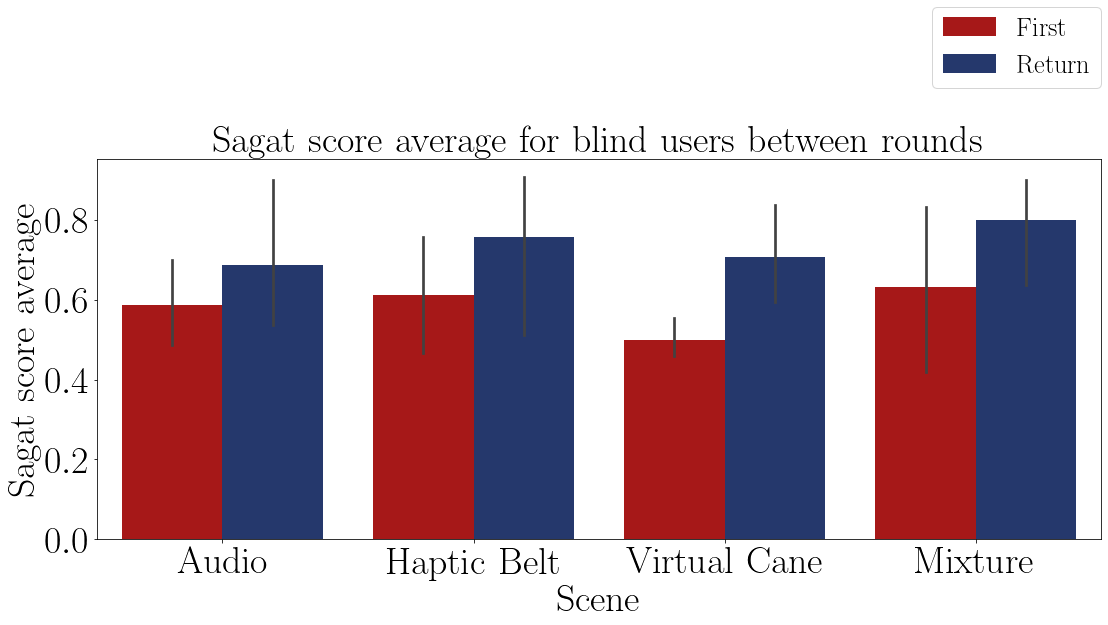
\includegraphics[width = 0.8\linewidth]{Resultados/Sagat/Figuras/png/barplot_sagat_avg_scene_blind.png}
        %\resizebox{0.6\linewidth}{!}{
        %%% Creator: Matplotlib, PGF backend
%%
%% To include the figure in your LaTeX document, write
%%   \input{<filename>.pgf}
%%
%% Make sure the required packages are loaded in your preamble
%%   \usepackage{pgf}
%%
%% Figures using additional raster images can only be included by \input if
%% they are in the same directory as the main LaTeX file. For loading figures
%% from other directories you can use the `import` package
%%   \usepackage{import}
%%
%% and then include the figures with
%%   \import{<path to file>}{<filename>.pgf}
%%
%% Matplotlib used the following preamble
%%   \usepackage{url}
%%   \usepackage{unicode-math}
%%   \setmainfont{DejaVu Serif}
%%   \usepackage{fontspec}
%%
\begingroup%
\makeatletter%
\begin{pgfpicture}%
\pgfpathrectangle{\pgfpointorigin}{\pgfqpoint{14.214174in}{5.669751in}}%
\pgfusepath{use as bounding box, clip}%
\begin{pgfscope}%
\pgfsetbuttcap%
\pgfsetmiterjoin%
\pgfsetlinewidth{0.000000pt}%
\definecolor{currentstroke}{rgb}{1.000000,1.000000,1.000000}%
\pgfsetstrokecolor{currentstroke}%
\pgfsetstrokeopacity{0.000000}%
\pgfsetdash{}{0pt}%
\pgfpathmoveto{\pgfqpoint{0.000000in}{0.000000in}}%
\pgfpathlineto{\pgfqpoint{14.214174in}{0.000000in}}%
\pgfpathlineto{\pgfqpoint{14.214174in}{5.669751in}}%
\pgfpathlineto{\pgfqpoint{0.000000in}{5.669751in}}%
\pgfpathclose%
\pgfusepath{}%
\end{pgfscope}%
\begin{pgfscope}%
\pgfsetbuttcap%
\pgfsetmiterjoin%
\definecolor{currentfill}{rgb}{1.000000,1.000000,1.000000}%
\pgfsetfillcolor{currentfill}%
\pgfsetlinewidth{0.000000pt}%
\definecolor{currentstroke}{rgb}{0.000000,0.000000,0.000000}%
\pgfsetstrokecolor{currentstroke}%
\pgfsetstrokeopacity{0.000000}%
\pgfsetdash{}{0pt}%
\pgfpathmoveto{\pgfqpoint{4.782087in}{1.324875in}}%
\pgfpathlineto{\pgfqpoint{9.432087in}{1.324875in}}%
\pgfpathlineto{\pgfqpoint{9.432087in}{4.344875in}}%
\pgfpathlineto{\pgfqpoint{4.782087in}{4.344875in}}%
\pgfpathclose%
\pgfusepath{fill}%
\end{pgfscope}%
\begin{pgfscope}%
\pgfpathrectangle{\pgfqpoint{4.782087in}{1.324875in}}{\pgfqpoint{4.650000in}{3.020000in}}%
\pgfusepath{clip}%
\pgfsetbuttcap%
\pgfsetmiterjoin%
\definecolor{currentfill}{rgb}{0.651961,0.093137,0.093137}%
\pgfsetfillcolor{currentfill}%
\pgfsetlinewidth{0.000000pt}%
\definecolor{currentstroke}{rgb}{0.000000,0.000000,0.000000}%
\pgfsetstrokecolor{currentstroke}%
\pgfsetstrokeopacity{0.000000}%
\pgfsetdash{}{0pt}%
\pgfpathmoveto{\pgfqpoint{4.898337in}{1.324875in}}%
\pgfpathlineto{\pgfqpoint{5.363337in}{1.324875in}}%
\pgfpathlineto{\pgfqpoint{5.363337in}{3.189440in}}%
\pgfpathlineto{\pgfqpoint{4.898337in}{3.189440in}}%
\pgfpathclose%
\pgfusepath{fill}%
\end{pgfscope}%
\begin{pgfscope}%
\pgfpathrectangle{\pgfqpoint{4.782087in}{1.324875in}}{\pgfqpoint{4.650000in}{3.020000in}}%
\pgfusepath{clip}%
\pgfsetbuttcap%
\pgfsetmiterjoin%
\definecolor{currentfill}{rgb}{0.651961,0.093137,0.093137}%
\pgfsetfillcolor{currentfill}%
\pgfsetlinewidth{0.000000pt}%
\definecolor{currentstroke}{rgb}{0.000000,0.000000,0.000000}%
\pgfsetstrokecolor{currentstroke}%
\pgfsetstrokeopacity{0.000000}%
\pgfsetdash{}{0pt}%
\pgfpathmoveto{\pgfqpoint{6.060837in}{1.324875in}}%
\pgfpathlineto{\pgfqpoint{6.525837in}{1.324875in}}%
\pgfpathlineto{\pgfqpoint{6.525837in}{3.266403in}}%
\pgfpathlineto{\pgfqpoint{6.060837in}{3.266403in}}%
\pgfpathclose%
\pgfusepath{fill}%
\end{pgfscope}%
\begin{pgfscope}%
\pgfpathrectangle{\pgfqpoint{4.782087in}{1.324875in}}{\pgfqpoint{4.650000in}{3.020000in}}%
\pgfusepath{clip}%
\pgfsetbuttcap%
\pgfsetmiterjoin%
\definecolor{currentfill}{rgb}{0.651961,0.093137,0.093137}%
\pgfsetfillcolor{currentfill}%
\pgfsetlinewidth{0.000000pt}%
\definecolor{currentstroke}{rgb}{0.000000,0.000000,0.000000}%
\pgfsetstrokecolor{currentstroke}%
\pgfsetstrokeopacity{0.000000}%
\pgfsetdash{}{0pt}%
\pgfpathmoveto{\pgfqpoint{7.223337in}{1.324875in}}%
\pgfpathlineto{\pgfqpoint{7.688337in}{1.324875in}}%
\pgfpathlineto{\pgfqpoint{7.688337in}{2.910152in}}%
\pgfpathlineto{\pgfqpoint{7.223337in}{2.910152in}}%
\pgfpathclose%
\pgfusepath{fill}%
\end{pgfscope}%
\begin{pgfscope}%
\pgfpathrectangle{\pgfqpoint{4.782087in}{1.324875in}}{\pgfqpoint{4.650000in}{3.020000in}}%
\pgfusepath{clip}%
\pgfsetbuttcap%
\pgfsetmiterjoin%
\definecolor{currentfill}{rgb}{0.651961,0.093137,0.093137}%
\pgfsetfillcolor{currentfill}%
\pgfsetlinewidth{0.000000pt}%
\definecolor{currentstroke}{rgb}{0.000000,0.000000,0.000000}%
\pgfsetstrokecolor{currentstroke}%
\pgfsetstrokeopacity{0.000000}%
\pgfsetdash{}{0pt}%
\pgfpathmoveto{\pgfqpoint{8.385837in}{1.324875in}}%
\pgfpathlineto{\pgfqpoint{8.850837in}{1.324875in}}%
\pgfpathlineto{\pgfqpoint{8.850837in}{3.328291in}}%
\pgfpathlineto{\pgfqpoint{8.385837in}{3.328291in}}%
\pgfpathclose%
\pgfusepath{fill}%
\end{pgfscope}%
\begin{pgfscope}%
\pgfpathrectangle{\pgfqpoint{4.782087in}{1.324875in}}{\pgfqpoint{4.650000in}{3.020000in}}%
\pgfusepath{clip}%
\pgfsetbuttcap%
\pgfsetmiterjoin%
\definecolor{currentfill}{rgb}{0.144608,0.218137,0.424020}%
\pgfsetfillcolor{currentfill}%
\pgfsetlinewidth{0.000000pt}%
\definecolor{currentstroke}{rgb}{0.000000,0.000000,0.000000}%
\pgfsetstrokecolor{currentstroke}%
\pgfsetstrokeopacity{0.000000}%
\pgfsetdash{}{0pt}%
\pgfpathmoveto{\pgfqpoint{5.363337in}{1.324875in}}%
\pgfpathlineto{\pgfqpoint{5.828337in}{1.324875in}}%
\pgfpathlineto{\pgfqpoint{5.828337in}{3.506813in}}%
\pgfpathlineto{\pgfqpoint{5.363337in}{3.506813in}}%
\pgfpathclose%
\pgfusepath{fill}%
\end{pgfscope}%
\begin{pgfscope}%
\pgfpathrectangle{\pgfqpoint{4.782087in}{1.324875in}}{\pgfqpoint{4.650000in}{3.020000in}}%
\pgfusepath{clip}%
\pgfsetbuttcap%
\pgfsetmiterjoin%
\definecolor{currentfill}{rgb}{0.144608,0.218137,0.424020}%
\pgfsetfillcolor{currentfill}%
\pgfsetlinewidth{0.000000pt}%
\definecolor{currentstroke}{rgb}{0.000000,0.000000,0.000000}%
\pgfsetstrokecolor{currentstroke}%
\pgfsetstrokeopacity{0.000000}%
\pgfsetdash{}{0pt}%
\pgfpathmoveto{\pgfqpoint{6.525837in}{1.324875in}}%
\pgfpathlineto{\pgfqpoint{6.990837in}{1.324875in}}%
\pgfpathlineto{\pgfqpoint{6.990837in}{3.725007in}}%
\pgfpathlineto{\pgfqpoint{6.525837in}{3.725007in}}%
\pgfpathclose%
\pgfusepath{fill}%
\end{pgfscope}%
\begin{pgfscope}%
\pgfpathrectangle{\pgfqpoint{4.782087in}{1.324875in}}{\pgfqpoint{4.650000in}{3.020000in}}%
\pgfusepath{clip}%
\pgfsetbuttcap%
\pgfsetmiterjoin%
\definecolor{currentfill}{rgb}{0.144608,0.218137,0.424020}%
\pgfsetfillcolor{currentfill}%
\pgfsetlinewidth{0.000000pt}%
\definecolor{currentstroke}{rgb}{0.000000,0.000000,0.000000}%
\pgfsetstrokecolor{currentstroke}%
\pgfsetstrokeopacity{0.000000}%
\pgfsetdash{}{0pt}%
\pgfpathmoveto{\pgfqpoint{7.688337in}{1.324875in}}%
\pgfpathlineto{\pgfqpoint{8.153337in}{1.324875in}}%
\pgfpathlineto{\pgfqpoint{8.153337in}{3.566320in}}%
\pgfpathlineto{\pgfqpoint{7.688337in}{3.566320in}}%
\pgfpathclose%
\pgfusepath{fill}%
\end{pgfscope}%
\begin{pgfscope}%
\pgfpathrectangle{\pgfqpoint{4.782087in}{1.324875in}}{\pgfqpoint{4.650000in}{3.020000in}}%
\pgfusepath{clip}%
\pgfsetbuttcap%
\pgfsetmiterjoin%
\definecolor{currentfill}{rgb}{0.144608,0.218137,0.424020}%
\pgfsetfillcolor{currentfill}%
\pgfsetlinewidth{0.000000pt}%
\definecolor{currentstroke}{rgb}{0.000000,0.000000,0.000000}%
\pgfsetstrokecolor{currentstroke}%
\pgfsetstrokeopacity{0.000000}%
\pgfsetdash{}{0pt}%
\pgfpathmoveto{\pgfqpoint{8.850837in}{1.324875in}}%
\pgfpathlineto{\pgfqpoint{9.315837in}{1.324875in}}%
\pgfpathlineto{\pgfqpoint{9.315837in}{3.863857in}}%
\pgfpathlineto{\pgfqpoint{8.850837in}{3.863857in}}%
\pgfpathclose%
\pgfusepath{fill}%
\end{pgfscope}%
\begin{pgfscope}%
\pgfsetbuttcap%
\pgfsetroundjoin%
\definecolor{currentfill}{rgb}{0.000000,0.000000,0.000000}%
\pgfsetfillcolor{currentfill}%
\pgfsetlinewidth{0.803000pt}%
\definecolor{currentstroke}{rgb}{0.000000,0.000000,0.000000}%
\pgfsetstrokecolor{currentstroke}%
\pgfsetdash{}{0pt}%
\pgfsys@defobject{currentmarker}{\pgfqpoint{0.000000in}{-0.048611in}}{\pgfqpoint{0.000000in}{0.000000in}}{%
\pgfpathmoveto{\pgfqpoint{0.000000in}{0.000000in}}%
\pgfpathlineto{\pgfqpoint{0.000000in}{-0.048611in}}%
\pgfusepath{stroke,fill}%
}%
\begin{pgfscope}%
\pgfsys@transformshift{5.363337in}{1.324875in}%
\pgfsys@useobject{currentmarker}{}%
\end{pgfscope}%
\end{pgfscope}%
\begin{pgfscope}%
\definecolor{textcolor}{rgb}{0.000000,0.000000,0.000000}%
\pgfsetstrokecolor{textcolor}%
\pgfsetfillcolor{textcolor}%
\pgftext[x=5.363337in,y=1.227653in,,top]{\color{textcolor}\rmfamily\fontsize{38.016000}{45.619200}\selectfont Audio}%
\end{pgfscope}%
\begin{pgfscope}%
\pgfsetbuttcap%
\pgfsetroundjoin%
\definecolor{currentfill}{rgb}{0.000000,0.000000,0.000000}%
\pgfsetfillcolor{currentfill}%
\pgfsetlinewidth{0.803000pt}%
\definecolor{currentstroke}{rgb}{0.000000,0.000000,0.000000}%
\pgfsetstrokecolor{currentstroke}%
\pgfsetdash{}{0pt}%
\pgfsys@defobject{currentmarker}{\pgfqpoint{0.000000in}{-0.048611in}}{\pgfqpoint{0.000000in}{0.000000in}}{%
\pgfpathmoveto{\pgfqpoint{0.000000in}{0.000000in}}%
\pgfpathlineto{\pgfqpoint{0.000000in}{-0.048611in}}%
\pgfusepath{stroke,fill}%
}%
\begin{pgfscope}%
\pgfsys@transformshift{6.525837in}{1.324875in}%
\pgfsys@useobject{currentmarker}{}%
\end{pgfscope}%
\end{pgfscope}%
\begin{pgfscope}%
\definecolor{textcolor}{rgb}{0.000000,0.000000,0.000000}%
\pgfsetstrokecolor{textcolor}%
\pgfsetfillcolor{textcolor}%
\pgftext[x=6.525837in,y=1.227653in,,top]{\color{textcolor}\rmfamily\fontsize{38.016000}{45.619200}\selectfont Haptic Belt}%
\end{pgfscope}%
\begin{pgfscope}%
\pgfsetbuttcap%
\pgfsetroundjoin%
\definecolor{currentfill}{rgb}{0.000000,0.000000,0.000000}%
\pgfsetfillcolor{currentfill}%
\pgfsetlinewidth{0.803000pt}%
\definecolor{currentstroke}{rgb}{0.000000,0.000000,0.000000}%
\pgfsetstrokecolor{currentstroke}%
\pgfsetdash{}{0pt}%
\pgfsys@defobject{currentmarker}{\pgfqpoint{0.000000in}{-0.048611in}}{\pgfqpoint{0.000000in}{0.000000in}}{%
\pgfpathmoveto{\pgfqpoint{0.000000in}{0.000000in}}%
\pgfpathlineto{\pgfqpoint{0.000000in}{-0.048611in}}%
\pgfusepath{stroke,fill}%
}%
\begin{pgfscope}%
\pgfsys@transformshift{7.688337in}{1.324875in}%
\pgfsys@useobject{currentmarker}{}%
\end{pgfscope}%
\end{pgfscope}%
\begin{pgfscope}%
\definecolor{textcolor}{rgb}{0.000000,0.000000,0.000000}%
\pgfsetstrokecolor{textcolor}%
\pgfsetfillcolor{textcolor}%
\pgftext[x=7.688337in,y=1.227653in,,top]{\color{textcolor}\rmfamily\fontsize{38.016000}{45.619200}\selectfont Virtual Cane}%
\end{pgfscope}%
\begin{pgfscope}%
\pgfsetbuttcap%
\pgfsetroundjoin%
\definecolor{currentfill}{rgb}{0.000000,0.000000,0.000000}%
\pgfsetfillcolor{currentfill}%
\pgfsetlinewidth{0.803000pt}%
\definecolor{currentstroke}{rgb}{0.000000,0.000000,0.000000}%
\pgfsetstrokecolor{currentstroke}%
\pgfsetdash{}{0pt}%
\pgfsys@defobject{currentmarker}{\pgfqpoint{0.000000in}{-0.048611in}}{\pgfqpoint{0.000000in}{0.000000in}}{%
\pgfpathmoveto{\pgfqpoint{0.000000in}{0.000000in}}%
\pgfpathlineto{\pgfqpoint{0.000000in}{-0.048611in}}%
\pgfusepath{stroke,fill}%
}%
\begin{pgfscope}%
\pgfsys@transformshift{8.850837in}{1.324875in}%
\pgfsys@useobject{currentmarker}{}%
\end{pgfscope}%
\end{pgfscope}%
\begin{pgfscope}%
\definecolor{textcolor}{rgb}{0.000000,0.000000,0.000000}%
\pgfsetstrokecolor{textcolor}%
\pgfsetfillcolor{textcolor}%
\pgftext[x=8.850837in,y=1.227653in,,top]{\color{textcolor}\rmfamily\fontsize{38.016000}{45.619200}\selectfont Mixture}%
\end{pgfscope}%
\begin{pgfscope}%
\definecolor{textcolor}{rgb}{0.000000,0.000000,0.000000}%
\pgfsetstrokecolor{textcolor}%
\pgfsetfillcolor{textcolor}%
\pgftext[x=7.107087in,y=0.661113in,,top]{\color{textcolor}\rmfamily\fontsize{38.016000}{45.619200}\selectfont Scene}%
\end{pgfscope}%
\begin{pgfscope}%
\pgfsetbuttcap%
\pgfsetroundjoin%
\definecolor{currentfill}{rgb}{0.000000,0.000000,0.000000}%
\pgfsetfillcolor{currentfill}%
\pgfsetlinewidth{0.803000pt}%
\definecolor{currentstroke}{rgb}{0.000000,0.000000,0.000000}%
\pgfsetstrokecolor{currentstroke}%
\pgfsetdash{}{0pt}%
\pgfsys@defobject{currentmarker}{\pgfqpoint{-0.048611in}{0.000000in}}{\pgfqpoint{-0.000000in}{0.000000in}}{%
\pgfpathmoveto{\pgfqpoint{-0.000000in}{0.000000in}}%
\pgfpathlineto{\pgfqpoint{-0.048611in}{0.000000in}}%
\pgfusepath{stroke,fill}%
}%
\begin{pgfscope}%
\pgfsys@transformshift{4.782087in}{1.324875in}%
\pgfsys@useobject{currentmarker}{}%
\end{pgfscope}%
\end{pgfscope}%
\begin{pgfscope}%
\definecolor{textcolor}{rgb}{0.000000,0.000000,0.000000}%
\pgfsetstrokecolor{textcolor}%
\pgfsetfillcolor{textcolor}%
\pgftext[x=4.010080in, y=1.124297in, left, base]{\color{textcolor}\rmfamily\fontsize{38.016000}{45.619200}\selectfont \(\displaystyle {0.0}\)}%
\end{pgfscope}%
\begin{pgfscope}%
\pgfsetbuttcap%
\pgfsetroundjoin%
\definecolor{currentfill}{rgb}{0.000000,0.000000,0.000000}%
\pgfsetfillcolor{currentfill}%
\pgfsetlinewidth{0.803000pt}%
\definecolor{currentstroke}{rgb}{0.000000,0.000000,0.000000}%
\pgfsetstrokecolor{currentstroke}%
\pgfsetdash{}{0pt}%
\pgfsys@defobject{currentmarker}{\pgfqpoint{-0.048611in}{0.000000in}}{\pgfqpoint{-0.000000in}{0.000000in}}{%
\pgfpathmoveto{\pgfqpoint{-0.000000in}{0.000000in}}%
\pgfpathlineto{\pgfqpoint{-0.048611in}{0.000000in}}%
\pgfusepath{stroke,fill}%
}%
\begin{pgfscope}%
\pgfsys@transformshift{4.782087in}{2.911739in}%
\pgfsys@useobject{currentmarker}{}%
\end{pgfscope}%
\end{pgfscope}%
\begin{pgfscope}%
\definecolor{textcolor}{rgb}{0.000000,0.000000,0.000000}%
\pgfsetstrokecolor{textcolor}%
\pgfsetfillcolor{textcolor}%
\pgftext[x=4.010080in, y=2.711161in, left, base]{\color{textcolor}\rmfamily\fontsize{38.016000}{45.619200}\selectfont \(\displaystyle {0.5}\)}%
\end{pgfscope}%
\begin{pgfscope}%
\definecolor{textcolor}{rgb}{0.000000,0.000000,0.000000}%
\pgfsetstrokecolor{textcolor}%
\pgfsetfillcolor{textcolor}%
\pgftext[x=3.954525in,y=2.834875in,,bottom,rotate=90.000000]{\color{textcolor}\rmfamily\fontsize{38.016000}{45.619200}\selectfont Sagat score average}%
\end{pgfscope}%
\begin{pgfscope}%
\pgfpathrectangle{\pgfqpoint{4.782087in}{1.324875in}}{\pgfqpoint{4.650000in}{3.020000in}}%
\pgfusepath{clip}%
\pgfsetrectcap%
\pgfsetroundjoin%
\pgfsetlinewidth{2.710125pt}%
\definecolor{currentstroke}{rgb}{0.260000,0.260000,0.260000}%
\pgfsetstrokecolor{currentstroke}%
\pgfsetdash{}{0pt}%
\pgfpathmoveto{\pgfqpoint{5.130837in}{2.872068in}}%
\pgfpathlineto{\pgfqpoint{5.130837in}{3.546485in}}%
\pgfusepath{stroke}%
\end{pgfscope}%
\begin{pgfscope}%
\pgfpathrectangle{\pgfqpoint{4.782087in}{1.324875in}}{\pgfqpoint{4.650000in}{3.020000in}}%
\pgfusepath{clip}%
\pgfsetrectcap%
\pgfsetroundjoin%
\pgfsetlinewidth{2.710125pt}%
\definecolor{currentstroke}{rgb}{0.260000,0.260000,0.260000}%
\pgfsetstrokecolor{currentstroke}%
\pgfsetdash{}{0pt}%
\pgfpathmoveto{\pgfqpoint{6.293337in}{2.803832in}}%
\pgfpathlineto{\pgfqpoint{6.293337in}{3.742462in}}%
\pgfusepath{stroke}%
\end{pgfscope}%
\begin{pgfscope}%
\pgfpathrectangle{\pgfqpoint{4.782087in}{1.324875in}}{\pgfqpoint{4.650000in}{3.020000in}}%
\pgfusepath{clip}%
\pgfsetrectcap%
\pgfsetroundjoin%
\pgfsetlinewidth{2.710125pt}%
\definecolor{currentstroke}{rgb}{0.260000,0.260000,0.260000}%
\pgfsetstrokecolor{currentstroke}%
\pgfsetdash{}{0pt}%
\pgfpathmoveto{\pgfqpoint{7.455837in}{2.765748in}}%
\pgfpathlineto{\pgfqpoint{7.455837in}{3.082327in}}%
\pgfusepath{stroke}%
\end{pgfscope}%
\begin{pgfscope}%
\pgfpathrectangle{\pgfqpoint{4.782087in}{1.324875in}}{\pgfqpoint{4.650000in}{3.020000in}}%
\pgfusepath{clip}%
\pgfsetrectcap%
\pgfsetroundjoin%
\pgfsetlinewidth{2.710125pt}%
\definecolor{currentstroke}{rgb}{0.260000,0.260000,0.260000}%
\pgfsetstrokecolor{currentstroke}%
\pgfsetdash{}{0pt}%
\pgfpathmoveto{\pgfqpoint{8.618337in}{2.653874in}}%
\pgfpathlineto{\pgfqpoint{8.618337in}{3.963036in}}%
\pgfusepath{stroke}%
\end{pgfscope}%
\begin{pgfscope}%
\pgfpathrectangle{\pgfqpoint{4.782087in}{1.324875in}}{\pgfqpoint{4.650000in}{3.020000in}}%
\pgfusepath{clip}%
\pgfsetrectcap%
\pgfsetroundjoin%
\pgfsetlinewidth{2.710125pt}%
\definecolor{currentstroke}{rgb}{0.260000,0.260000,0.260000}%
\pgfsetstrokecolor{currentstroke}%
\pgfsetdash{}{0pt}%
\pgfpathmoveto{\pgfqpoint{5.595837in}{3.030754in}}%
\pgfpathlineto{\pgfqpoint{5.595837in}{4.182222in}}%
\pgfusepath{stroke}%
\end{pgfscope}%
\begin{pgfscope}%
\pgfpathrectangle{\pgfqpoint{4.782087in}{1.324875in}}{\pgfqpoint{4.650000in}{3.020000in}}%
\pgfusepath{clip}%
\pgfsetrectcap%
\pgfsetroundjoin%
\pgfsetlinewidth{2.710125pt}%
\definecolor{currentstroke}{rgb}{0.260000,0.260000,0.260000}%
\pgfsetstrokecolor{currentstroke}%
\pgfsetdash{}{0pt}%
\pgfpathmoveto{\pgfqpoint{6.758337in}{2.951411in}}%
\pgfpathlineto{\pgfqpoint{6.758337in}{4.201066in}}%
\pgfusepath{stroke}%
\end{pgfscope}%
\begin{pgfscope}%
\pgfpathrectangle{\pgfqpoint{4.782087in}{1.324875in}}{\pgfqpoint{4.650000in}{3.020000in}}%
\pgfusepath{clip}%
\pgfsetrectcap%
\pgfsetroundjoin%
\pgfsetlinewidth{2.710125pt}%
\definecolor{currentstroke}{rgb}{0.260000,0.260000,0.260000}%
\pgfsetstrokecolor{currentstroke}%
\pgfsetdash{}{0pt}%
\pgfpathmoveto{\pgfqpoint{7.920837in}{3.209276in}}%
\pgfpathlineto{\pgfqpoint{7.920837in}{3.982872in}}%
\pgfusepath{stroke}%
\end{pgfscope}%
\begin{pgfscope}%
\pgfpathrectangle{\pgfqpoint{4.782087in}{1.324875in}}{\pgfqpoint{4.650000in}{3.020000in}}%
\pgfusepath{clip}%
\pgfsetrectcap%
\pgfsetroundjoin%
\pgfsetlinewidth{2.710125pt}%
\definecolor{currentstroke}{rgb}{0.260000,0.260000,0.260000}%
\pgfsetstrokecolor{currentstroke}%
\pgfsetdash{}{0pt}%
\pgfpathmoveto{\pgfqpoint{9.083337in}{3.348127in}}%
\pgfpathlineto{\pgfqpoint{9.083337in}{4.181230in}}%
\pgfusepath{stroke}%
\end{pgfscope}%
\begin{pgfscope}%
\pgfsetrectcap%
\pgfsetmiterjoin%
\pgfsetlinewidth{0.803000pt}%
\definecolor{currentstroke}{rgb}{0.000000,0.000000,0.000000}%
\pgfsetstrokecolor{currentstroke}%
\pgfsetdash{}{0pt}%
\pgfpathmoveto{\pgfqpoint{4.782087in}{1.324875in}}%
\pgfpathlineto{\pgfqpoint{4.782087in}{4.344875in}}%
\pgfusepath{stroke}%
\end{pgfscope}%
\begin{pgfscope}%
\pgfsetrectcap%
\pgfsetmiterjoin%
\pgfsetlinewidth{0.803000pt}%
\definecolor{currentstroke}{rgb}{0.000000,0.000000,0.000000}%
\pgfsetstrokecolor{currentstroke}%
\pgfsetdash{}{0pt}%
\pgfpathmoveto{\pgfqpoint{9.432087in}{1.324875in}}%
\pgfpathlineto{\pgfqpoint{9.432087in}{4.344875in}}%
\pgfusepath{stroke}%
\end{pgfscope}%
\begin{pgfscope}%
\pgfsetrectcap%
\pgfsetmiterjoin%
\pgfsetlinewidth{0.803000pt}%
\definecolor{currentstroke}{rgb}{0.000000,0.000000,0.000000}%
\pgfsetstrokecolor{currentstroke}%
\pgfsetdash{}{0pt}%
\pgfpathmoveto{\pgfqpoint{4.782087in}{1.324875in}}%
\pgfpathlineto{\pgfqpoint{9.432087in}{1.324875in}}%
\pgfusepath{stroke}%
\end{pgfscope}%
\begin{pgfscope}%
\pgfsetrectcap%
\pgfsetmiterjoin%
\pgfsetlinewidth{0.803000pt}%
\definecolor{currentstroke}{rgb}{0.000000,0.000000,0.000000}%
\pgfsetstrokecolor{currentstroke}%
\pgfsetdash{}{0pt}%
\pgfpathmoveto{\pgfqpoint{4.782087in}{4.344875in}}%
\pgfpathlineto{\pgfqpoint{9.432087in}{4.344875in}}%
\pgfusepath{stroke}%
\end{pgfscope}%
\begin{pgfscope}%
\definecolor{textcolor}{rgb}{0.000000,0.000000,0.000000}%
\pgfsetstrokecolor{textcolor}%
\pgfsetfillcolor{textcolor}%
\pgftext[x=7.107087in,y=4.462180in,,base]{\color{textcolor}\rmfamily\fontsize{38.016000}{45.619200}\selectfont Sagat score average for blind users between rounds}%
\end{pgfscope}%
\begin{pgfscope}%
\pgfsetbuttcap%
\pgfsetmiterjoin%
\definecolor{currentfill}{rgb}{1.000000,1.000000,1.000000}%
\pgfsetfillcolor{currentfill}%
\pgfsetfillopacity{0.800000}%
\pgfsetlinewidth{1.003750pt}%
\definecolor{currentstroke}{rgb}{0.800000,0.800000,0.800000}%
\pgfsetstrokecolor{currentstroke}%
\pgfsetstrokeopacity{0.800000}%
\pgfsetdash{}{0pt}%
\pgfpathmoveto{\pgfqpoint{6.897432in}{3.943708in}}%
\pgfpathlineto{\pgfqpoint{9.358754in}{3.943708in}}%
\pgfpathquadraticcurveto{\pgfqpoint{9.432087in}{3.943708in}}{\pgfqpoint{9.432087in}{4.017042in}}%
\pgfpathlineto{\pgfqpoint{9.432087in}{5.056742in}}%
\pgfpathquadraticcurveto{\pgfqpoint{9.432087in}{5.130075in}}{\pgfqpoint{9.358754in}{5.130075in}}%
\pgfpathlineto{\pgfqpoint{6.897432in}{5.130075in}}%
\pgfpathquadraticcurveto{\pgfqpoint{6.824099in}{5.130075in}}{\pgfqpoint{6.824099in}{5.056742in}}%
\pgfpathlineto{\pgfqpoint{6.824099in}{4.017042in}}%
\pgfpathquadraticcurveto{\pgfqpoint{6.824099in}{3.943708in}}{\pgfqpoint{6.897432in}{3.943708in}}%
\pgfpathclose%
\pgfusepath{stroke,fill}%
\end{pgfscope}%
\begin{pgfscope}%
\pgfsetbuttcap%
\pgfsetmiterjoin%
\definecolor{currentfill}{rgb}{0.651961,0.093137,0.093137}%
\pgfsetfillcolor{currentfill}%
\pgfsetlinewidth{0.000000pt}%
\definecolor{currentstroke}{rgb}{0.000000,0.000000,0.000000}%
\pgfsetstrokecolor{currentstroke}%
\pgfsetstrokeopacity{0.000000}%
\pgfsetdash{}{0pt}%
\pgfpathmoveto{\pgfqpoint{6.970766in}{4.704828in}}%
\pgfpathlineto{\pgfqpoint{7.704099in}{4.704828in}}%
\pgfpathlineto{\pgfqpoint{7.704099in}{4.961495in}}%
\pgfpathlineto{\pgfqpoint{6.970766in}{4.961495in}}%
\pgfpathclose%
\pgfusepath{fill}%
\end{pgfscope}%
\begin{pgfscope}%
\definecolor{textcolor}{rgb}{0.000000,0.000000,0.000000}%
\pgfsetstrokecolor{textcolor}%
\pgfsetfillcolor{textcolor}%
\pgftext[x=7.997432in,y=4.704828in,left,base]{\color{textcolor}\rmfamily\fontsize{26.400000}{31.680000}\selectfont First}%
\end{pgfscope}%
\begin{pgfscope}%
\pgfsetbuttcap%
\pgfsetmiterjoin%
\definecolor{currentfill}{rgb}{0.144608,0.218137,0.424020}%
\pgfsetfillcolor{currentfill}%
\pgfsetlinewidth{0.000000pt}%
\definecolor{currentstroke}{rgb}{0.000000,0.000000,0.000000}%
\pgfsetstrokecolor{currentstroke}%
\pgfsetstrokeopacity{0.000000}%
\pgfsetdash{}{0pt}%
\pgfpathmoveto{\pgfqpoint{6.970766in}{4.166644in}}%
\pgfpathlineto{\pgfqpoint{7.704099in}{4.166644in}}%
\pgfpathlineto{\pgfqpoint{7.704099in}{4.423311in}}%
\pgfpathlineto{\pgfqpoint{6.970766in}{4.423311in}}%
\pgfpathclose%
\pgfusepath{fill}%
\end{pgfscope}%
\begin{pgfscope}%
\definecolor{textcolor}{rgb}{0.000000,0.000000,0.000000}%
\pgfsetstrokecolor{textcolor}%
\pgfsetfillcolor{textcolor}%
\pgftext[x=7.997432in,y=4.166644in,left,base]{\color{textcolor}\rmfamily\fontsize{26.400000}{31.680000}\selectfont Return}%
\end{pgfscope}%
\end{pgfpicture}%
\makeatother%
\endgroup%
    
        %}
        \caption{Bar plot of the average Sagat score of the blind participants on each method.}
        \label{fig:barplot_sagat_scene_blind}
    \end{minipage}
    \begin{minipage}{\textwidth}
        \centering
        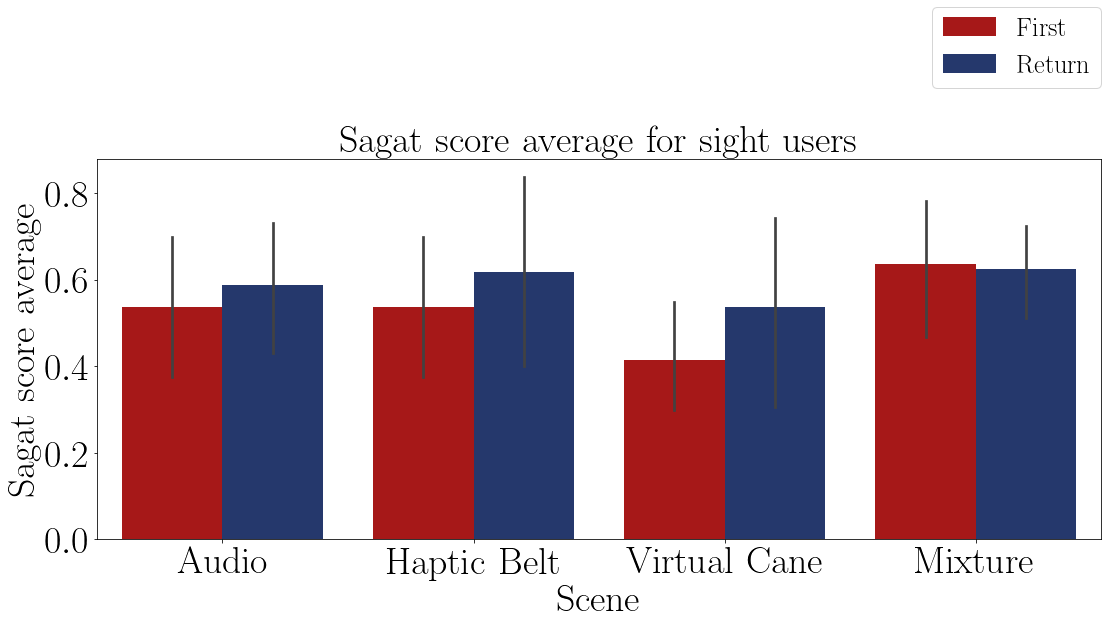
\includegraphics[width = 0.8\linewidth]{Resultados/Sagat/Figuras/png/barplot_sagat_avg_scene_sight.png}
        %\resizebox{0.6\linewidth}{!}{
        %%% Creator: Matplotlib, PGF backend
%%
%% To include the figure in your LaTeX document, write
%%   \input{<filename>.pgf}
%%
%% Make sure the required packages are loaded in your preamble
%%   \usepackage{pgf}
%%
%% Figures using additional raster images can only be included by \input if
%% they are in the same directory as the main LaTeX file. For loading figures
%% from other directories you can use the `import` package
%%   \usepackage{import}
%%
%% and then include the figures with
%%   \import{<path to file>}{<filename>.pgf}
%%
%% Matplotlib used the following preamble
%%   \usepackage{fontspec}
%%
\begingroup%
\makeatletter%
\begin{pgfpicture}%
\pgfpathrectangle{\pgfpointorigin}{\pgfqpoint{15.190505in}{8.690562in}}%
\pgfusepath{use as bounding box, clip}%
\begin{pgfscope}%
\pgfsetbuttcap%
\pgfsetmiterjoin%
\pgfsetlinewidth{0.000000pt}%
\definecolor{currentstroke}{rgb}{1.000000,1.000000,1.000000}%
\pgfsetstrokecolor{currentstroke}%
\pgfsetstrokeopacity{0.000000}%
\pgfsetdash{}{0pt}%
\pgfpathmoveto{\pgfqpoint{0.000000in}{-0.000000in}}%
\pgfpathlineto{\pgfqpoint{15.190505in}{-0.000000in}}%
\pgfpathlineto{\pgfqpoint{15.190505in}{8.690562in}}%
\pgfpathlineto{\pgfqpoint{0.000000in}{8.690562in}}%
\pgfpathclose%
\pgfusepath{}%
\end{pgfscope}%
\begin{pgfscope}%
\pgfsetbuttcap%
\pgfsetmiterjoin%
\definecolor{currentfill}{rgb}{1.000000,1.000000,1.000000}%
\pgfsetfillcolor{currentfill}%
\pgfsetlinewidth{0.000000pt}%
\definecolor{currentstroke}{rgb}{0.000000,0.000000,0.000000}%
\pgfsetstrokecolor{currentstroke}%
\pgfsetstrokeopacity{0.000000}%
\pgfsetdash{}{0pt}%
\pgfpathmoveto{\pgfqpoint{1.140505in}{1.191562in}}%
\pgfpathlineto{\pgfqpoint{15.090505in}{1.191562in}}%
\pgfpathlineto{\pgfqpoint{15.090505in}{6.476562in}}%
\pgfpathlineto{\pgfqpoint{1.140505in}{6.476562in}}%
\pgfpathclose%
\pgfusepath{fill}%
\end{pgfscope}%
\begin{pgfscope}%
\pgfpathrectangle{\pgfqpoint{1.140505in}{1.191562in}}{\pgfqpoint{13.950000in}{5.285000in}}%
\pgfusepath{clip}%
\pgfsetbuttcap%
\pgfsetmiterjoin%
\definecolor{currentfill}{rgb}{0.651961,0.093137,0.093137}%
\pgfsetfillcolor{currentfill}%
\pgfsetlinewidth{0.000000pt}%
\definecolor{currentstroke}{rgb}{0.000000,0.000000,0.000000}%
\pgfsetstrokecolor{currentstroke}%
\pgfsetstrokeopacity{0.000000}%
\pgfsetdash{}{0pt}%
\pgfpathmoveto{\pgfqpoint{1.489255in}{1.191562in}}%
\pgfpathlineto{\pgfqpoint{2.884255in}{1.191562in}}%
\pgfpathlineto{\pgfqpoint{2.884255in}{4.421910in}}%
\pgfpathlineto{\pgfqpoint{1.489255in}{4.421910in}}%
\pgfpathclose%
\pgfusepath{fill}%
\end{pgfscope}%
\begin{pgfscope}%
\pgfpathrectangle{\pgfqpoint{1.140505in}{1.191562in}}{\pgfqpoint{13.950000in}{5.285000in}}%
\pgfusepath{clip}%
\pgfsetbuttcap%
\pgfsetmiterjoin%
\definecolor{currentfill}{rgb}{0.651961,0.093137,0.093137}%
\pgfsetfillcolor{currentfill}%
\pgfsetlinewidth{0.000000pt}%
\definecolor{currentstroke}{rgb}{0.000000,0.000000,0.000000}%
\pgfsetstrokecolor{currentstroke}%
\pgfsetstrokeopacity{0.000000}%
\pgfsetdash{}{0pt}%
\pgfpathmoveto{\pgfqpoint{4.976755in}{1.191562in}}%
\pgfpathlineto{\pgfqpoint{6.371755in}{1.191562in}}%
\pgfpathlineto{\pgfqpoint{6.371755in}{4.417402in}}%
\pgfpathlineto{\pgfqpoint{4.976755in}{4.417402in}}%
\pgfpathclose%
\pgfusepath{fill}%
\end{pgfscope}%
\begin{pgfscope}%
\pgfpathrectangle{\pgfqpoint{1.140505in}{1.191562in}}{\pgfqpoint{13.950000in}{5.285000in}}%
\pgfusepath{clip}%
\pgfsetbuttcap%
\pgfsetmiterjoin%
\definecolor{currentfill}{rgb}{0.651961,0.093137,0.093137}%
\pgfsetfillcolor{currentfill}%
\pgfsetlinewidth{0.000000pt}%
\definecolor{currentstroke}{rgb}{0.000000,0.000000,0.000000}%
\pgfsetstrokecolor{currentstroke}%
\pgfsetstrokeopacity{0.000000}%
\pgfsetdash{}{0pt}%
\pgfpathmoveto{\pgfqpoint{8.464255in}{1.191562in}}%
\pgfpathlineto{\pgfqpoint{9.859255in}{1.191562in}}%
\pgfpathlineto{\pgfqpoint{9.859255in}{3.690198in}}%
\pgfpathlineto{\pgfqpoint{8.464255in}{3.690198in}}%
\pgfpathclose%
\pgfusepath{fill}%
\end{pgfscope}%
\begin{pgfscope}%
\pgfpathrectangle{\pgfqpoint{1.140505in}{1.191562in}}{\pgfqpoint{13.950000in}{5.285000in}}%
\pgfusepath{clip}%
\pgfsetbuttcap%
\pgfsetmiterjoin%
\definecolor{currentfill}{rgb}{0.651961,0.093137,0.093137}%
\pgfsetfillcolor{currentfill}%
\pgfsetlinewidth{0.000000pt}%
\definecolor{currentstroke}{rgb}{0.000000,0.000000,0.000000}%
\pgfsetstrokecolor{currentstroke}%
\pgfsetstrokeopacity{0.000000}%
\pgfsetdash{}{0pt}%
\pgfpathmoveto{\pgfqpoint{11.951755in}{1.191562in}}%
\pgfpathlineto{\pgfqpoint{13.346755in}{1.191562in}}%
\pgfpathlineto{\pgfqpoint{13.346755in}{5.022905in}}%
\pgfpathlineto{\pgfqpoint{11.951755in}{5.022905in}}%
\pgfpathclose%
\pgfusepath{fill}%
\end{pgfscope}%
\begin{pgfscope}%
\pgfpathrectangle{\pgfqpoint{1.140505in}{1.191562in}}{\pgfqpoint{13.950000in}{5.285000in}}%
\pgfusepath{clip}%
\pgfsetbuttcap%
\pgfsetmiterjoin%
\definecolor{currentfill}{rgb}{0.144608,0.218137,0.424020}%
\pgfsetfillcolor{currentfill}%
\pgfsetlinewidth{0.000000pt}%
\definecolor{currentstroke}{rgb}{0.000000,0.000000,0.000000}%
\pgfsetstrokecolor{currentstroke}%
\pgfsetstrokeopacity{0.000000}%
\pgfsetdash{}{0pt}%
\pgfpathmoveto{\pgfqpoint{2.884255in}{1.191562in}}%
\pgfpathlineto{\pgfqpoint{4.279255in}{1.191562in}}%
\pgfpathlineto{\pgfqpoint{4.279255in}{4.722407in}}%
\pgfpathlineto{\pgfqpoint{2.884255in}{4.722407in}}%
\pgfpathclose%
\pgfusepath{fill}%
\end{pgfscope}%
\begin{pgfscope}%
\pgfpathrectangle{\pgfqpoint{1.140505in}{1.191562in}}{\pgfqpoint{13.950000in}{5.285000in}}%
\pgfusepath{clip}%
\pgfsetbuttcap%
\pgfsetmiterjoin%
\definecolor{currentfill}{rgb}{0.144608,0.218137,0.424020}%
\pgfsetfillcolor{currentfill}%
\pgfsetlinewidth{0.000000pt}%
\definecolor{currentstroke}{rgb}{0.000000,0.000000,0.000000}%
\pgfsetstrokecolor{currentstroke}%
\pgfsetstrokeopacity{0.000000}%
\pgfsetdash{}{0pt}%
\pgfpathmoveto{\pgfqpoint{6.371755in}{1.191562in}}%
\pgfpathlineto{\pgfqpoint{7.766755in}{1.191562in}}%
\pgfpathlineto{\pgfqpoint{7.766755in}{4.910218in}}%
\pgfpathlineto{\pgfqpoint{6.371755in}{4.910218in}}%
\pgfpathclose%
\pgfusepath{fill}%
\end{pgfscope}%
\begin{pgfscope}%
\pgfpathrectangle{\pgfqpoint{1.140505in}{1.191562in}}{\pgfqpoint{13.950000in}{5.285000in}}%
\pgfusepath{clip}%
\pgfsetbuttcap%
\pgfsetmiterjoin%
\definecolor{currentfill}{rgb}{0.144608,0.218137,0.424020}%
\pgfsetfillcolor{currentfill}%
\pgfsetlinewidth{0.000000pt}%
\definecolor{currentstroke}{rgb}{0.000000,0.000000,0.000000}%
\pgfsetstrokecolor{currentstroke}%
\pgfsetstrokeopacity{0.000000}%
\pgfsetdash{}{0pt}%
\pgfpathmoveto{\pgfqpoint{9.859255in}{1.191562in}}%
\pgfpathlineto{\pgfqpoint{11.254255in}{1.191562in}}%
\pgfpathlineto{\pgfqpoint{11.254255in}{4.421910in}}%
\pgfpathlineto{\pgfqpoint{9.859255in}{4.421910in}}%
\pgfpathclose%
\pgfusepath{fill}%
\end{pgfscope}%
\begin{pgfscope}%
\pgfpathrectangle{\pgfqpoint{1.140505in}{1.191562in}}{\pgfqpoint{13.950000in}{5.285000in}}%
\pgfusepath{clip}%
\pgfsetbuttcap%
\pgfsetmiterjoin%
\definecolor{currentfill}{rgb}{0.144608,0.218137,0.424020}%
\pgfsetfillcolor{currentfill}%
\pgfsetlinewidth{0.000000pt}%
\definecolor{currentstroke}{rgb}{0.000000,0.000000,0.000000}%
\pgfsetstrokecolor{currentstroke}%
\pgfsetstrokeopacity{0.000000}%
\pgfsetdash{}{0pt}%
\pgfpathmoveto{\pgfqpoint{13.346755in}{1.191562in}}%
\pgfpathlineto{\pgfqpoint{14.741755in}{1.191562in}}%
\pgfpathlineto{\pgfqpoint{14.741755in}{4.947781in}}%
\pgfpathlineto{\pgfqpoint{13.346755in}{4.947781in}}%
\pgfpathclose%
\pgfusepath{fill}%
\end{pgfscope}%
\begin{pgfscope}%
\pgfsetbuttcap%
\pgfsetroundjoin%
\definecolor{currentfill}{rgb}{0.000000,0.000000,0.000000}%
\pgfsetfillcolor{currentfill}%
\pgfsetlinewidth{0.803000pt}%
\definecolor{currentstroke}{rgb}{0.000000,0.000000,0.000000}%
\pgfsetstrokecolor{currentstroke}%
\pgfsetdash{}{0pt}%
\pgfsys@defobject{currentmarker}{\pgfqpoint{0.000000in}{-0.048611in}}{\pgfqpoint{0.000000in}{0.000000in}}{%
\pgfpathmoveto{\pgfqpoint{0.000000in}{0.000000in}}%
\pgfpathlineto{\pgfqpoint{0.000000in}{-0.048611in}}%
\pgfusepath{stroke,fill}%
}%
\begin{pgfscope}%
\pgfsys@transformshift{2.884255in}{1.191562in}%
\pgfsys@useobject{currentmarker}{}%
\end{pgfscope}%
\end{pgfscope}%
\begin{pgfscope}%
\definecolor{textcolor}{rgb}{0.000000,0.000000,0.000000}%
\pgfsetstrokecolor{textcolor}%
\pgfsetfillcolor{textcolor}%
\pgftext[x=2.884255in,y=1.094339in,,top]{\color{textcolor}\rmfamily\fontsize{38.016000}{45.619200}\selectfont Audio}%
\end{pgfscope}%
\begin{pgfscope}%
\pgfsetbuttcap%
\pgfsetroundjoin%
\definecolor{currentfill}{rgb}{0.000000,0.000000,0.000000}%
\pgfsetfillcolor{currentfill}%
\pgfsetlinewidth{0.803000pt}%
\definecolor{currentstroke}{rgb}{0.000000,0.000000,0.000000}%
\pgfsetstrokecolor{currentstroke}%
\pgfsetdash{}{0pt}%
\pgfsys@defobject{currentmarker}{\pgfqpoint{0.000000in}{-0.048611in}}{\pgfqpoint{0.000000in}{0.000000in}}{%
\pgfpathmoveto{\pgfqpoint{0.000000in}{0.000000in}}%
\pgfpathlineto{\pgfqpoint{0.000000in}{-0.048611in}}%
\pgfusepath{stroke,fill}%
}%
\begin{pgfscope}%
\pgfsys@transformshift{6.371755in}{1.191562in}%
\pgfsys@useobject{currentmarker}{}%
\end{pgfscope}%
\end{pgfscope}%
\begin{pgfscope}%
\definecolor{textcolor}{rgb}{0.000000,0.000000,0.000000}%
\pgfsetstrokecolor{textcolor}%
\pgfsetfillcolor{textcolor}%
\pgftext[x=6.371755in,y=1.094339in,,top]{\color{textcolor}\rmfamily\fontsize{38.016000}{45.619200}\selectfont Haptic Belt}%
\end{pgfscope}%
\begin{pgfscope}%
\pgfsetbuttcap%
\pgfsetroundjoin%
\definecolor{currentfill}{rgb}{0.000000,0.000000,0.000000}%
\pgfsetfillcolor{currentfill}%
\pgfsetlinewidth{0.803000pt}%
\definecolor{currentstroke}{rgb}{0.000000,0.000000,0.000000}%
\pgfsetstrokecolor{currentstroke}%
\pgfsetdash{}{0pt}%
\pgfsys@defobject{currentmarker}{\pgfqpoint{0.000000in}{-0.048611in}}{\pgfqpoint{0.000000in}{0.000000in}}{%
\pgfpathmoveto{\pgfqpoint{0.000000in}{0.000000in}}%
\pgfpathlineto{\pgfqpoint{0.000000in}{-0.048611in}}%
\pgfusepath{stroke,fill}%
}%
\begin{pgfscope}%
\pgfsys@transformshift{9.859255in}{1.191562in}%
\pgfsys@useobject{currentmarker}{}%
\end{pgfscope}%
\end{pgfscope}%
\begin{pgfscope}%
\definecolor{textcolor}{rgb}{0.000000,0.000000,0.000000}%
\pgfsetstrokecolor{textcolor}%
\pgfsetfillcolor{textcolor}%
\pgftext[x=9.859255in,y=1.094339in,,top]{\color{textcolor}\rmfamily\fontsize{38.016000}{45.619200}\selectfont Virtual Cane}%
\end{pgfscope}%
\begin{pgfscope}%
\pgfsetbuttcap%
\pgfsetroundjoin%
\definecolor{currentfill}{rgb}{0.000000,0.000000,0.000000}%
\pgfsetfillcolor{currentfill}%
\pgfsetlinewidth{0.803000pt}%
\definecolor{currentstroke}{rgb}{0.000000,0.000000,0.000000}%
\pgfsetstrokecolor{currentstroke}%
\pgfsetdash{}{0pt}%
\pgfsys@defobject{currentmarker}{\pgfqpoint{0.000000in}{-0.048611in}}{\pgfqpoint{0.000000in}{0.000000in}}{%
\pgfpathmoveto{\pgfqpoint{0.000000in}{0.000000in}}%
\pgfpathlineto{\pgfqpoint{0.000000in}{-0.048611in}}%
\pgfusepath{stroke,fill}%
}%
\begin{pgfscope}%
\pgfsys@transformshift{13.346755in}{1.191562in}%
\pgfsys@useobject{currentmarker}{}%
\end{pgfscope}%
\end{pgfscope}%
\begin{pgfscope}%
\definecolor{textcolor}{rgb}{0.000000,0.000000,0.000000}%
\pgfsetstrokecolor{textcolor}%
\pgfsetfillcolor{textcolor}%
\pgftext[x=13.346755in,y=1.094339in,,top]{\color{textcolor}\rmfamily\fontsize{38.016000}{45.619200}\selectfont Mixture}%
\end{pgfscope}%
\begin{pgfscope}%
\definecolor{textcolor}{rgb}{0.000000,0.000000,0.000000}%
\pgfsetstrokecolor{textcolor}%
\pgfsetfillcolor{textcolor}%
\pgftext[x=8.115505in,y=0.569392in,,top]{\color{textcolor}\rmfamily\fontsize{38.016000}{45.619200}\selectfont Scene}%
\end{pgfscope}%
\begin{pgfscope}%
\pgfsetbuttcap%
\pgfsetroundjoin%
\definecolor{currentfill}{rgb}{0.000000,0.000000,0.000000}%
\pgfsetfillcolor{currentfill}%
\pgfsetlinewidth{0.803000pt}%
\definecolor{currentstroke}{rgb}{0.000000,0.000000,0.000000}%
\pgfsetstrokecolor{currentstroke}%
\pgfsetdash{}{0pt}%
\pgfsys@defobject{currentmarker}{\pgfqpoint{-0.048611in}{0.000000in}}{\pgfqpoint{-0.000000in}{0.000000in}}{%
\pgfpathmoveto{\pgfqpoint{-0.000000in}{0.000000in}}%
\pgfpathlineto{\pgfqpoint{-0.048611in}{0.000000in}}%
\pgfusepath{stroke,fill}%
}%
\begin{pgfscope}%
\pgfsys@transformshift{1.140505in}{1.191562in}%
\pgfsys@useobject{currentmarker}{}%
\end{pgfscope}%
\end{pgfscope}%
\begin{pgfscope}%
\definecolor{textcolor}{rgb}{0.000000,0.000000,0.000000}%
\pgfsetstrokecolor{textcolor}%
\pgfsetfillcolor{textcolor}%
\pgftext[x=0.632340in, y=1.008346in, left, base]{\color{textcolor}\rmfamily\fontsize{38.016000}{45.619200}\selectfont \(\displaystyle {0.0}\)}%
\end{pgfscope}%
\begin{pgfscope}%
\pgfsetbuttcap%
\pgfsetroundjoin%
\definecolor{currentfill}{rgb}{0.000000,0.000000,0.000000}%
\pgfsetfillcolor{currentfill}%
\pgfsetlinewidth{0.803000pt}%
\definecolor{currentstroke}{rgb}{0.000000,0.000000,0.000000}%
\pgfsetstrokecolor{currentstroke}%
\pgfsetdash{}{0pt}%
\pgfsys@defobject{currentmarker}{\pgfqpoint{-0.048611in}{0.000000in}}{\pgfqpoint{-0.000000in}{0.000000in}}{%
\pgfpathmoveto{\pgfqpoint{-0.000000in}{0.000000in}}%
\pgfpathlineto{\pgfqpoint{-0.048611in}{0.000000in}}%
\pgfusepath{stroke,fill}%
}%
\begin{pgfscope}%
\pgfsys@transformshift{1.140505in}{2.393552in}%
\pgfsys@useobject{currentmarker}{}%
\end{pgfscope}%
\end{pgfscope}%
\begin{pgfscope}%
\definecolor{textcolor}{rgb}{0.000000,0.000000,0.000000}%
\pgfsetstrokecolor{textcolor}%
\pgfsetfillcolor{textcolor}%
\pgftext[x=0.632340in, y=2.210336in, left, base]{\color{textcolor}\rmfamily\fontsize{38.016000}{45.619200}\selectfont \(\displaystyle {0.2}\)}%
\end{pgfscope}%
\begin{pgfscope}%
\pgfsetbuttcap%
\pgfsetroundjoin%
\definecolor{currentfill}{rgb}{0.000000,0.000000,0.000000}%
\pgfsetfillcolor{currentfill}%
\pgfsetlinewidth{0.803000pt}%
\definecolor{currentstroke}{rgb}{0.000000,0.000000,0.000000}%
\pgfsetstrokecolor{currentstroke}%
\pgfsetdash{}{0pt}%
\pgfsys@defobject{currentmarker}{\pgfqpoint{-0.048611in}{0.000000in}}{\pgfqpoint{-0.000000in}{0.000000in}}{%
\pgfpathmoveto{\pgfqpoint{-0.000000in}{0.000000in}}%
\pgfpathlineto{\pgfqpoint{-0.048611in}{0.000000in}}%
\pgfusepath{stroke,fill}%
}%
\begin{pgfscope}%
\pgfsys@transformshift{1.140505in}{3.595542in}%
\pgfsys@useobject{currentmarker}{}%
\end{pgfscope}%
\end{pgfscope}%
\begin{pgfscope}%
\definecolor{textcolor}{rgb}{0.000000,0.000000,0.000000}%
\pgfsetstrokecolor{textcolor}%
\pgfsetfillcolor{textcolor}%
\pgftext[x=0.632340in, y=3.412326in, left, base]{\color{textcolor}\rmfamily\fontsize{38.016000}{45.619200}\selectfont \(\displaystyle {0.4}\)}%
\end{pgfscope}%
\begin{pgfscope}%
\pgfsetbuttcap%
\pgfsetroundjoin%
\definecolor{currentfill}{rgb}{0.000000,0.000000,0.000000}%
\pgfsetfillcolor{currentfill}%
\pgfsetlinewidth{0.803000pt}%
\definecolor{currentstroke}{rgb}{0.000000,0.000000,0.000000}%
\pgfsetstrokecolor{currentstroke}%
\pgfsetdash{}{0pt}%
\pgfsys@defobject{currentmarker}{\pgfqpoint{-0.048611in}{0.000000in}}{\pgfqpoint{-0.000000in}{0.000000in}}{%
\pgfpathmoveto{\pgfqpoint{-0.000000in}{0.000000in}}%
\pgfpathlineto{\pgfqpoint{-0.048611in}{0.000000in}}%
\pgfusepath{stroke,fill}%
}%
\begin{pgfscope}%
\pgfsys@transformshift{1.140505in}{4.797532in}%
\pgfsys@useobject{currentmarker}{}%
\end{pgfscope}%
\end{pgfscope}%
\begin{pgfscope}%
\definecolor{textcolor}{rgb}{0.000000,0.000000,0.000000}%
\pgfsetstrokecolor{textcolor}%
\pgfsetfillcolor{textcolor}%
\pgftext[x=0.632340in, y=4.614316in, left, base]{\color{textcolor}\rmfamily\fontsize{38.016000}{45.619200}\selectfont \(\displaystyle {0.6}\)}%
\end{pgfscope}%
\begin{pgfscope}%
\pgfsetbuttcap%
\pgfsetroundjoin%
\definecolor{currentfill}{rgb}{0.000000,0.000000,0.000000}%
\pgfsetfillcolor{currentfill}%
\pgfsetlinewidth{0.803000pt}%
\definecolor{currentstroke}{rgb}{0.000000,0.000000,0.000000}%
\pgfsetstrokecolor{currentstroke}%
\pgfsetdash{}{0pt}%
\pgfsys@defobject{currentmarker}{\pgfqpoint{-0.048611in}{0.000000in}}{\pgfqpoint{-0.000000in}{0.000000in}}{%
\pgfpathmoveto{\pgfqpoint{-0.000000in}{0.000000in}}%
\pgfpathlineto{\pgfqpoint{-0.048611in}{0.000000in}}%
\pgfusepath{stroke,fill}%
}%
\begin{pgfscope}%
\pgfsys@transformshift{1.140505in}{5.999522in}%
\pgfsys@useobject{currentmarker}{}%
\end{pgfscope}%
\end{pgfscope}%
\begin{pgfscope}%
\definecolor{textcolor}{rgb}{0.000000,0.000000,0.000000}%
\pgfsetstrokecolor{textcolor}%
\pgfsetfillcolor{textcolor}%
\pgftext[x=0.632340in, y=5.816306in, left, base]{\color{textcolor}\rmfamily\fontsize{38.016000}{45.619200}\selectfont \(\displaystyle {0.8}\)}%
\end{pgfscope}%
\begin{pgfscope}%
\definecolor{textcolor}{rgb}{0.000000,0.000000,0.000000}%
\pgfsetstrokecolor{textcolor}%
\pgfsetfillcolor{textcolor}%
\pgftext[x=0.576784in,y=3.834062in,,bottom,rotate=90.000000]{\color{textcolor}\rmfamily\fontsize{38.016000}{45.619200}\selectfont Sagat score average}%
\end{pgfscope}%
\begin{pgfscope}%
\pgfpathrectangle{\pgfqpoint{1.140505in}{1.191562in}}{\pgfqpoint{13.950000in}{5.285000in}}%
\pgfusepath{clip}%
\pgfsetrectcap%
\pgfsetroundjoin%
\pgfsetlinewidth{2.710125pt}%
\definecolor{currentstroke}{rgb}{0.260000,0.260000,0.260000}%
\pgfsetstrokecolor{currentstroke}%
\pgfsetdash{}{0pt}%
\pgfpathmoveto{\pgfqpoint{2.186755in}{3.445293in}}%
\pgfpathlineto{\pgfqpoint{2.186755in}{5.398527in}}%
\pgfusepath{stroke}%
\end{pgfscope}%
\begin{pgfscope}%
\pgfpathrectangle{\pgfqpoint{1.140505in}{1.191562in}}{\pgfqpoint{13.950000in}{5.285000in}}%
\pgfusepath{clip}%
\pgfsetrectcap%
\pgfsetroundjoin%
\pgfsetlinewidth{2.710125pt}%
\definecolor{currentstroke}{rgb}{0.260000,0.260000,0.260000}%
\pgfsetstrokecolor{currentstroke}%
\pgfsetdash{}{0pt}%
\pgfpathmoveto{\pgfqpoint{5.674255in}{3.442288in}}%
\pgfpathlineto{\pgfqpoint{5.674255in}{5.443601in}}%
\pgfusepath{stroke}%
\end{pgfscope}%
\begin{pgfscope}%
\pgfpathrectangle{\pgfqpoint{1.140505in}{1.191562in}}{\pgfqpoint{13.950000in}{5.285000in}}%
\pgfusepath{clip}%
\pgfsetrectcap%
\pgfsetroundjoin%
\pgfsetlinewidth{2.710125pt}%
\definecolor{currentstroke}{rgb}{0.260000,0.260000,0.260000}%
\pgfsetstrokecolor{currentstroke}%
\pgfsetdash{}{0pt}%
\pgfpathmoveto{\pgfqpoint{9.161755in}{2.990039in}}%
\pgfpathlineto{\pgfqpoint{9.161755in}{4.491024in}}%
\pgfusepath{stroke}%
\end{pgfscope}%
\begin{pgfscope}%
\pgfpathrectangle{\pgfqpoint{1.140505in}{1.191562in}}{\pgfqpoint{13.950000in}{5.285000in}}%
\pgfusepath{clip}%
\pgfsetrectcap%
\pgfsetroundjoin%
\pgfsetlinewidth{2.710125pt}%
\definecolor{currentstroke}{rgb}{0.260000,0.260000,0.260000}%
\pgfsetstrokecolor{currentstroke}%
\pgfsetdash{}{0pt}%
\pgfpathmoveto{\pgfqpoint{12.649255in}{4.008726in}}%
\pgfpathlineto{\pgfqpoint{12.649255in}{5.886835in}}%
\pgfusepath{stroke}%
\end{pgfscope}%
\begin{pgfscope}%
\pgfpathrectangle{\pgfqpoint{1.140505in}{1.191562in}}{\pgfqpoint{13.950000in}{5.285000in}}%
\pgfusepath{clip}%
\pgfsetrectcap%
\pgfsetroundjoin%
\pgfsetlinewidth{2.710125pt}%
\definecolor{currentstroke}{rgb}{0.260000,0.260000,0.260000}%
\pgfsetstrokecolor{currentstroke}%
\pgfsetdash{}{0pt}%
\pgfpathmoveto{\pgfqpoint{3.581755in}{3.783353in}}%
\pgfpathlineto{\pgfqpoint{3.581755in}{5.586338in}}%
\pgfusepath{stroke}%
\end{pgfscope}%
\begin{pgfscope}%
\pgfpathrectangle{\pgfqpoint{1.140505in}{1.191562in}}{\pgfqpoint{13.950000in}{5.285000in}}%
\pgfusepath{clip}%
\pgfsetrectcap%
\pgfsetroundjoin%
\pgfsetlinewidth{2.710125pt}%
\definecolor{currentstroke}{rgb}{0.260000,0.260000,0.260000}%
\pgfsetstrokecolor{currentstroke}%
\pgfsetdash{}{0pt}%
\pgfpathmoveto{\pgfqpoint{7.069255in}{3.595542in}}%
\pgfpathlineto{\pgfqpoint{7.069255in}{6.224895in}}%
\pgfusepath{stroke}%
\end{pgfscope}%
\begin{pgfscope}%
\pgfpathrectangle{\pgfqpoint{1.140505in}{1.191562in}}{\pgfqpoint{13.950000in}{5.285000in}}%
\pgfusepath{clip}%
\pgfsetrectcap%
\pgfsetroundjoin%
\pgfsetlinewidth{2.710125pt}%
\definecolor{currentstroke}{rgb}{0.260000,0.260000,0.260000}%
\pgfsetstrokecolor{currentstroke}%
\pgfsetdash{}{0pt}%
\pgfpathmoveto{\pgfqpoint{10.556755in}{2.844298in}}%
\pgfpathlineto{\pgfqpoint{10.556755in}{5.661462in}}%
\pgfusepath{stroke}%
\end{pgfscope}%
\begin{pgfscope}%
\pgfpathrectangle{\pgfqpoint{1.140505in}{1.191562in}}{\pgfqpoint{13.950000in}{5.285000in}}%
\pgfusepath{clip}%
\pgfsetrectcap%
\pgfsetroundjoin%
\pgfsetlinewidth{2.710125pt}%
\definecolor{currentstroke}{rgb}{0.260000,0.260000,0.260000}%
\pgfsetstrokecolor{currentstroke}%
\pgfsetdash{}{0pt}%
\pgfpathmoveto{\pgfqpoint{14.044255in}{4.271661in}}%
\pgfpathlineto{\pgfqpoint{14.044255in}{5.623900in}}%
\pgfusepath{stroke}%
\end{pgfscope}%
\begin{pgfscope}%
\pgfsetrectcap%
\pgfsetmiterjoin%
\pgfsetlinewidth{0.803000pt}%
\definecolor{currentstroke}{rgb}{0.000000,0.000000,0.000000}%
\pgfsetstrokecolor{currentstroke}%
\pgfsetdash{}{0pt}%
\pgfpathmoveto{\pgfqpoint{1.140505in}{1.191562in}}%
\pgfpathlineto{\pgfqpoint{1.140505in}{6.476562in}}%
\pgfusepath{stroke}%
\end{pgfscope}%
\begin{pgfscope}%
\pgfsetrectcap%
\pgfsetmiterjoin%
\pgfsetlinewidth{0.803000pt}%
\definecolor{currentstroke}{rgb}{0.000000,0.000000,0.000000}%
\pgfsetstrokecolor{currentstroke}%
\pgfsetdash{}{0pt}%
\pgfpathmoveto{\pgfqpoint{15.090505in}{1.191562in}}%
\pgfpathlineto{\pgfqpoint{15.090505in}{6.476562in}}%
\pgfusepath{stroke}%
\end{pgfscope}%
\begin{pgfscope}%
\pgfsetrectcap%
\pgfsetmiterjoin%
\pgfsetlinewidth{0.803000pt}%
\definecolor{currentstroke}{rgb}{0.000000,0.000000,0.000000}%
\pgfsetstrokecolor{currentstroke}%
\pgfsetdash{}{0pt}%
\pgfpathmoveto{\pgfqpoint{1.140505in}{1.191562in}}%
\pgfpathlineto{\pgfqpoint{15.090505in}{1.191562in}}%
\pgfusepath{stroke}%
\end{pgfscope}%
\begin{pgfscope}%
\pgfsetrectcap%
\pgfsetmiterjoin%
\pgfsetlinewidth{0.803000pt}%
\definecolor{currentstroke}{rgb}{0.000000,0.000000,0.000000}%
\pgfsetstrokecolor{currentstroke}%
\pgfsetdash{}{0pt}%
\pgfpathmoveto{\pgfqpoint{1.140505in}{6.476562in}}%
\pgfpathlineto{\pgfqpoint{15.090505in}{6.476562in}}%
\pgfusepath{stroke}%
\end{pgfscope}%
\begin{pgfscope}%
\definecolor{textcolor}{rgb}{0.000000,0.000000,0.000000}%
\pgfsetstrokecolor{textcolor}%
\pgfsetfillcolor{textcolor}%
\pgftext[x=8.115505in,y=6.584273in,,base]{\color{textcolor}\rmfamily\fontsize{38.016000}{45.619200}\selectfont Sagat score average for sight users}%
\end{pgfscope}%
\begin{pgfscope}%
\pgfsetbuttcap%
\pgfsetmiterjoin%
\definecolor{currentfill}{rgb}{1.000000,1.000000,1.000000}%
\pgfsetfillcolor{currentfill}%
\pgfsetfillopacity{0.800000}%
\pgfsetlinewidth{1.003750pt}%
\definecolor{currentstroke}{rgb}{0.800000,0.800000,0.800000}%
\pgfsetstrokecolor{currentstroke}%
\pgfsetstrokeopacity{0.800000}%
\pgfsetdash{}{0pt}%
\pgfpathmoveto{\pgfqpoint{12.811305in}{7.457562in}}%
\pgfpathlineto{\pgfqpoint{15.017171in}{7.457562in}}%
\pgfpathquadraticcurveto{\pgfqpoint{15.090505in}{7.457562in}}{\pgfqpoint{15.090505in}{7.530896in}}%
\pgfpathlineto{\pgfqpoint{15.090505in}{8.517228in}}%
\pgfpathquadraticcurveto{\pgfqpoint{15.090505in}{8.590562in}}{\pgfqpoint{15.017171in}{8.590562in}}%
\pgfpathlineto{\pgfqpoint{12.811305in}{8.590562in}}%
\pgfpathquadraticcurveto{\pgfqpoint{12.737972in}{8.590562in}}{\pgfqpoint{12.737972in}{8.517228in}}%
\pgfpathlineto{\pgfqpoint{12.737972in}{7.530896in}}%
\pgfpathquadraticcurveto{\pgfqpoint{12.737972in}{7.457562in}}{\pgfqpoint{12.811305in}{7.457562in}}%
\pgfpathclose%
\pgfusepath{stroke,fill}%
\end{pgfscope}%
\begin{pgfscope}%
\pgfsetbuttcap%
\pgfsetmiterjoin%
\definecolor{currentfill}{rgb}{0.651961,0.093137,0.093137}%
\pgfsetfillcolor{currentfill}%
\pgfsetlinewidth{0.000000pt}%
\definecolor{currentstroke}{rgb}{0.000000,0.000000,0.000000}%
\pgfsetstrokecolor{currentstroke}%
\pgfsetstrokeopacity{0.000000}%
\pgfsetdash{}{0pt}%
\pgfpathmoveto{\pgfqpoint{12.884638in}{8.187228in}}%
\pgfpathlineto{\pgfqpoint{13.617972in}{8.187228in}}%
\pgfpathlineto{\pgfqpoint{13.617972in}{8.443895in}}%
\pgfpathlineto{\pgfqpoint{12.884638in}{8.443895in}}%
\pgfpathclose%
\pgfusepath{fill}%
\end{pgfscope}%
\begin{pgfscope}%
\definecolor{textcolor}{rgb}{0.000000,0.000000,0.000000}%
\pgfsetstrokecolor{textcolor}%
\pgfsetfillcolor{textcolor}%
\pgftext[x=13.911305in,y=8.187228in,left,base]{\color{textcolor}\rmfamily\fontsize{26.400000}{31.680000}\selectfont First}%
\end{pgfscope}%
\begin{pgfscope}%
\pgfsetbuttcap%
\pgfsetmiterjoin%
\definecolor{currentfill}{rgb}{0.144608,0.218137,0.424020}%
\pgfsetfillcolor{currentfill}%
\pgfsetlinewidth{0.000000pt}%
\definecolor{currentstroke}{rgb}{0.000000,0.000000,0.000000}%
\pgfsetstrokecolor{currentstroke}%
\pgfsetstrokeopacity{0.000000}%
\pgfsetdash{}{0pt}%
\pgfpathmoveto{\pgfqpoint{12.884638in}{7.675729in}}%
\pgfpathlineto{\pgfqpoint{13.617972in}{7.675729in}}%
\pgfpathlineto{\pgfqpoint{13.617972in}{7.932395in}}%
\pgfpathlineto{\pgfqpoint{12.884638in}{7.932395in}}%
\pgfpathclose%
\pgfusepath{fill}%
\end{pgfscope}%
\begin{pgfscope}%
\definecolor{textcolor}{rgb}{0.000000,0.000000,0.000000}%
\pgfsetstrokecolor{textcolor}%
\pgfsetfillcolor{textcolor}%
\pgftext[x=13.911305in,y=7.675729in,left,base]{\color{textcolor}\rmfamily\fontsize{26.400000}{31.680000}\selectfont Return}%
\end{pgfscope}%
\end{pgfpicture}%
\makeatother%
\endgroup%
    
        %}
        \caption{Bar plot of the average Sagat score of the sighted participants on each method.}
        \label{fig:barplot_sagat_scene_sight}
    \end{minipage}
\end{figure}


The Table \ref{tab:sagat_average} show the the average Sagat score between the rounds of each participant and the Figure \ref{fig:boxplot_sagat_scene} these data is plotted. It is possible only to assume that some methods causes differente Sagat scores than other, but both groups performed rather similarly.


\begin{table}[!htb]
\centering
\caption{Adapted Sagat average global score grouped by participant and guidance method.}
\label{tab:sagat_average}
\begin{tabular}{lrrrrrr}
\toprule
{} &  Base & Audio & \begin{tabular}[c]{@{}l@{}}Haptic\\ Belt\end{tabular} & \begin{tabular}[c]{@{}l@{}}Virtual\\ Cane\end{tabular} & Mixture & \begin{tabular}[c]{@{}l@{}}Visual\\ Condition\end{tabular} \\
Participant &       &       &                                                       &                                                        &         &                                                            \\
\midrule
001         &  1.00 &  0.53 &                                                  0.47 &                                                   0.38 &    0.55 &                                                      Sight \\
001C        &  0.62 &  0.60 &                                                  0.69 &                                                   0.57 &    0.45 &                                                      Blind \\
002C        &  0.60 &  0.47 &                                                  0.40 &                                                   0.55 &    0.74 &                                                      Blind \\
003         &  1.00 &  0.64 &                                                  0.66 &                                                   0.51 &    0.71 &                                                      Sight \\
003C        &  0.86 &  0.88 &                                                  0.80 &                                                   0.68 &    0.90 &                                                      Blind \\
004         &  1.00 &  0.75 &                                                  0.87 &                                                   0.71 &    0.76 &                                                      Sight \\
004C        &  0.82 &  0.60 &                                                  0.85 &                                                   0.61 &    0.78 &                                                      Blind \\
005         &  1.00 &  0.34 &                                                  0.31 &                                                   0.30 &    0.50 &                                                      Sight \\
\bottomrule
\end{tabular}
\end{table}



%\begin{figure}[!htb]
%    \centering
%    \resizebox{0.6\linewidth}{!}{
%    %% Creator: Matplotlib, PGF backend
%%
%% To include the figure in your LaTeX document, write
%%   \input{<filename>.pgf}
%%
%% Make sure the required packages are loaded in your preamble
%%   \usepackage{pgf}
%%
%% and, on pdftex
%%   \usepackage[utf8]{inputenc}\DeclareUnicodeCharacter{2212}{-}
%%
%% or, on luatex and xetex
%%   \usepackage{unicode-math}
%%
%% Figures using additional raster images can only be included by \input if
%% they are in the same directory as the main LaTeX file. For loading figures
%% from other directories you can use the `import` package
%%   \usepackage{import}
%%
%% and then include the figures with
%%   \import{<path to file>}{<filename>.pgf}
%%
%% Matplotlib used the following preamble
%%   \usepackage{url}
%%   \usepackage{unicode-math}
%%   \setmainfont{DejaVu Serif}
%%   \usepackage{fontspec}
%%
\begingroup%
\makeatletter%
\begin{pgfpicture}%
\pgfpathrectangle{\pgfpointorigin}{\pgfqpoint{12.196638in}{14.528848in}}%
\pgfusepath{use as bounding box, clip}%
\begin{pgfscope}%
\pgfsetbuttcap%
\pgfsetmiterjoin%
\pgfsetlinewidth{0.000000pt}%
\definecolor{currentstroke}{rgb}{1.000000,1.000000,1.000000}%
\pgfsetstrokecolor{currentstroke}%
\pgfsetstrokeopacity{0.000000}%
\pgfsetdash{}{0pt}%
\pgfpathmoveto{\pgfqpoint{0.000000in}{0.000000in}}%
\pgfpathlineto{\pgfqpoint{12.196638in}{0.000000in}}%
\pgfpathlineto{\pgfqpoint{12.196638in}{14.528848in}}%
\pgfpathlineto{\pgfqpoint{0.000000in}{14.528848in}}%
\pgfpathclose%
\pgfusepath{}%
\end{pgfscope}%
\begin{pgfscope}%
\pgfsetbuttcap%
\pgfsetmiterjoin%
\definecolor{currentfill}{rgb}{1.000000,1.000000,1.000000}%
\pgfsetfillcolor{currentfill}%
\pgfsetlinewidth{0.000000pt}%
\definecolor{currentstroke}{rgb}{0.000000,0.000000,0.000000}%
\pgfsetstrokecolor{currentstroke}%
\pgfsetstrokeopacity{0.000000}%
\pgfsetdash{}{0pt}%
\pgfpathmoveto{\pgfqpoint{1.246638in}{1.110648in}}%
\pgfpathlineto{\pgfqpoint{12.096638in}{1.110648in}}%
\pgfpathlineto{\pgfqpoint{12.096638in}{11.680648in}}%
\pgfpathlineto{\pgfqpoint{1.246638in}{11.680648in}}%
\pgfpathclose%
\pgfusepath{fill}%
\end{pgfscope}%
\begin{pgfscope}%
\pgfpathrectangle{\pgfqpoint{1.246638in}{1.110648in}}{\pgfqpoint{10.850000in}{10.570000in}}%
\pgfusepath{clip}%
\pgfsetbuttcap%
\pgfsetmiterjoin%
\definecolor{currentfill}{rgb}{0.651961,0.093137,0.093137}%
\pgfsetfillcolor{currentfill}%
\pgfsetlinewidth{1.505625pt}%
\definecolor{currentstroke}{rgb}{0.168627,0.168627,0.168627}%
\pgfsetstrokecolor{currentstroke}%
\pgfsetdash{}{0pt}%
\pgfpathmoveto{\pgfqpoint{1.797818in}{11.200194in}}%
\pgfpathlineto{\pgfqpoint{2.648458in}{11.200194in}}%
\pgfpathlineto{\pgfqpoint{2.648458in}{11.200194in}}%
\pgfpathlineto{\pgfqpoint{1.797818in}{11.200194in}}%
\pgfpathlineto{\pgfqpoint{1.797818in}{11.200194in}}%
\pgfpathclose%
\pgfusepath{stroke,fill}%
\end{pgfscope}%
\begin{pgfscope}%
\pgfpathrectangle{\pgfqpoint{1.246638in}{1.110648in}}{\pgfqpoint{10.850000in}{10.570000in}}%
\pgfusepath{clip}%
\pgfsetbuttcap%
\pgfsetmiterjoin%
\definecolor{currentfill}{rgb}{0.144608,0.218137,0.424020}%
\pgfsetfillcolor{currentfill}%
\pgfsetlinewidth{1.505625pt}%
\definecolor{currentstroke}{rgb}{0.168627,0.168627,0.168627}%
\pgfsetstrokecolor{currentstroke}%
\pgfsetdash{}{0pt}%
\pgfpathmoveto{\pgfqpoint{2.665818in}{4.041387in}}%
\pgfpathlineto{\pgfqpoint{3.516458in}{4.041387in}}%
\pgfpathlineto{\pgfqpoint{3.516458in}{6.613413in}}%
\pgfpathlineto{\pgfqpoint{2.665818in}{6.613413in}}%
\pgfpathlineto{\pgfqpoint{2.665818in}{4.041387in}}%
\pgfpathclose%
\pgfusepath{stroke,fill}%
\end{pgfscope}%
\begin{pgfscope}%
\pgfpathrectangle{\pgfqpoint{1.246638in}{1.110648in}}{\pgfqpoint{10.850000in}{10.570000in}}%
\pgfusepath{clip}%
\pgfsetbuttcap%
\pgfsetmiterjoin%
\definecolor{currentfill}{rgb}{0.823529,0.823529,0.823529}%
\pgfsetfillcolor{currentfill}%
\pgfsetlinewidth{1.505625pt}%
\definecolor{currentstroke}{rgb}{0.168627,0.168627,0.168627}%
\pgfsetstrokecolor{currentstroke}%
\pgfsetdash{}{0pt}%
\pgfpathmoveto{\pgfqpoint{3.533818in}{3.338366in}}%
\pgfpathlineto{\pgfqpoint{4.384458in}{3.338366in}}%
\pgfpathlineto{\pgfqpoint{4.384458in}{7.292428in}}%
\pgfpathlineto{\pgfqpoint{3.533818in}{7.292428in}}%
\pgfpathlineto{\pgfqpoint{3.533818in}{3.338366in}}%
\pgfpathclose%
\pgfusepath{stroke,fill}%
\end{pgfscope}%
\begin{pgfscope}%
\pgfpathrectangle{\pgfqpoint{1.246638in}{1.110648in}}{\pgfqpoint{10.850000in}{10.570000in}}%
\pgfusepath{clip}%
\pgfsetbuttcap%
\pgfsetmiterjoin%
\definecolor{currentfill}{rgb}{0.875000,0.419118,0.125000}%
\pgfsetfillcolor{currentfill}%
\pgfsetlinewidth{1.505625pt}%
\definecolor{currentstroke}{rgb}{0.168627,0.168627,0.168627}%
\pgfsetstrokecolor{currentstroke}%
\pgfsetdash{}{0pt}%
\pgfpathmoveto{\pgfqpoint{4.401818in}{2.450160in}}%
\pgfpathlineto{\pgfqpoint{5.252458in}{2.450160in}}%
\pgfpathlineto{\pgfqpoint{5.252458in}{5.191940in}}%
\pgfpathlineto{\pgfqpoint{4.401818in}{5.191940in}}%
\pgfpathlineto{\pgfqpoint{4.401818in}{2.450160in}}%
\pgfpathclose%
\pgfusepath{stroke,fill}%
\end{pgfscope}%
\begin{pgfscope}%
\pgfpathrectangle{\pgfqpoint{1.246638in}{1.110648in}}{\pgfqpoint{10.850000in}{10.570000in}}%
\pgfusepath{clip}%
\pgfsetbuttcap%
\pgfsetmiterjoin%
\definecolor{currentfill}{rgb}{0.696078,0.784314,0.872549}%
\pgfsetfillcolor{currentfill}%
\pgfsetlinewidth{1.505625pt}%
\definecolor{currentstroke}{rgb}{0.168627,0.168627,0.168627}%
\pgfsetstrokecolor{currentstroke}%
\pgfsetdash{}{0pt}%
\pgfpathmoveto{\pgfqpoint{5.269818in}{4.855862in}}%
\pgfpathlineto{\pgfqpoint{6.120458in}{4.855862in}}%
\pgfpathlineto{\pgfqpoint{6.120458in}{7.427888in}}%
\pgfpathlineto{\pgfqpoint{5.269818in}{7.427888in}}%
\pgfpathlineto{\pgfqpoint{5.269818in}{4.855862in}}%
\pgfpathclose%
\pgfusepath{stroke,fill}%
\end{pgfscope}%
\begin{pgfscope}%
\pgfpathrectangle{\pgfqpoint{1.246638in}{1.110648in}}{\pgfqpoint{10.850000in}{10.570000in}}%
\pgfusepath{clip}%
\pgfsetbuttcap%
\pgfsetmiterjoin%
\definecolor{currentfill}{rgb}{0.651961,0.093137,0.093137}%
\pgfsetfillcolor{currentfill}%
\pgfsetlinewidth{1.505625pt}%
\definecolor{currentstroke}{rgb}{0.168627,0.168627,0.168627}%
\pgfsetstrokecolor{currentstroke}%
\pgfsetdash{}{0pt}%
\pgfpathmoveto{\pgfqpoint{7.222818in}{5.970407in}}%
\pgfpathlineto{\pgfqpoint{8.073458in}{5.970407in}}%
\pgfpathlineto{\pgfqpoint{8.073458in}{8.928237in}}%
\pgfpathlineto{\pgfqpoint{7.222818in}{8.928237in}}%
\pgfpathlineto{\pgfqpoint{7.222818in}{5.970407in}}%
\pgfpathclose%
\pgfusepath{stroke,fill}%
\end{pgfscope}%
\begin{pgfscope}%
\pgfpathrectangle{\pgfqpoint{1.246638in}{1.110648in}}{\pgfqpoint{10.850000in}{10.570000in}}%
\pgfusepath{clip}%
\pgfsetbuttcap%
\pgfsetmiterjoin%
\definecolor{currentfill}{rgb}{0.144608,0.218137,0.424020}%
\pgfsetfillcolor{currentfill}%
\pgfsetlinewidth{1.505625pt}%
\definecolor{currentstroke}{rgb}{0.168627,0.168627,0.168627}%
\pgfsetstrokecolor{currentstroke}%
\pgfsetdash{}{0pt}%
\pgfpathmoveto{\pgfqpoint{8.090818in}{5.284533in}}%
\pgfpathlineto{\pgfqpoint{8.941458in}{5.284533in}}%
\pgfpathlineto{\pgfqpoint{8.941458in}{6.656280in}}%
\pgfpathlineto{\pgfqpoint{8.090818in}{6.656280in}}%
\pgfpathlineto{\pgfqpoint{8.090818in}{5.284533in}}%
\pgfpathclose%
\pgfusepath{stroke,fill}%
\end{pgfscope}%
\begin{pgfscope}%
\pgfpathrectangle{\pgfqpoint{1.246638in}{1.110648in}}{\pgfqpoint{10.850000in}{10.570000in}}%
\pgfusepath{clip}%
\pgfsetbuttcap%
\pgfsetmiterjoin%
\definecolor{currentfill}{rgb}{0.823529,0.823529,0.823529}%
\pgfsetfillcolor{currentfill}%
\pgfsetlinewidth{1.505625pt}%
\definecolor{currentstroke}{rgb}{0.168627,0.168627,0.168627}%
\pgfsetstrokecolor{currentstroke}%
\pgfsetdash{}{0pt}%
\pgfpathmoveto{\pgfqpoint{8.958818in}{5.966977in}}%
\pgfpathlineto{\pgfqpoint{9.809458in}{5.966977in}}%
\pgfpathlineto{\pgfqpoint{9.809458in}{8.607591in}}%
\pgfpathlineto{\pgfqpoint{8.958818in}{8.607591in}}%
\pgfpathlineto{\pgfqpoint{8.958818in}{5.966977in}}%
\pgfpathclose%
\pgfusepath{stroke,fill}%
\end{pgfscope}%
\begin{pgfscope}%
\pgfpathrectangle{\pgfqpoint{1.246638in}{1.110648in}}{\pgfqpoint{10.850000in}{10.570000in}}%
\pgfusepath{clip}%
\pgfsetbuttcap%
\pgfsetmiterjoin%
\definecolor{currentfill}{rgb}{0.875000,0.419118,0.125000}%
\pgfsetfillcolor{currentfill}%
\pgfsetlinewidth{1.505625pt}%
\definecolor{currentstroke}{rgb}{0.168627,0.168627,0.168627}%
\pgfsetstrokecolor{currentstroke}%
\pgfsetdash{}{0pt}%
\pgfpathmoveto{\pgfqpoint{9.826818in}{5.197084in}}%
\pgfpathlineto{\pgfqpoint{10.677458in}{5.197084in}}%
\pgfpathlineto{\pgfqpoint{10.677458in}{6.121299in}}%
\pgfpathlineto{\pgfqpoint{9.826818in}{6.121299in}}%
\pgfpathlineto{\pgfqpoint{9.826818in}{5.197084in}}%
\pgfpathclose%
\pgfusepath{stroke,fill}%
\end{pgfscope}%
\begin{pgfscope}%
\pgfpathrectangle{\pgfqpoint{1.246638in}{1.110648in}}{\pgfqpoint{10.850000in}{10.570000in}}%
\pgfusepath{clip}%
\pgfsetbuttcap%
\pgfsetmiterjoin%
\definecolor{currentfill}{rgb}{0.696078,0.784314,0.872549}%
\pgfsetfillcolor{currentfill}%
\pgfsetlinewidth{1.505625pt}%
\definecolor{currentstroke}{rgb}{0.168627,0.168627,0.168627}%
\pgfsetstrokecolor{currentstroke}%
\pgfsetdash{}{0pt}%
\pgfpathmoveto{\pgfqpoint{10.694818in}{6.613413in}}%
\pgfpathlineto{\pgfqpoint{11.545458in}{6.613413in}}%
\pgfpathlineto{\pgfqpoint{11.545458in}{8.542433in}}%
\pgfpathlineto{\pgfqpoint{10.694818in}{8.542433in}}%
\pgfpathlineto{\pgfqpoint{10.694818in}{6.613413in}}%
\pgfpathclose%
\pgfusepath{stroke,fill}%
\end{pgfscope}%
\begin{pgfscope}%
\pgfpathrectangle{\pgfqpoint{1.246638in}{1.110648in}}{\pgfqpoint{10.850000in}{10.570000in}}%
\pgfusepath{clip}%
\pgfsetbuttcap%
\pgfsetmiterjoin%
\definecolor{currentfill}{rgb}{0.651961,0.093137,0.093137}%
\pgfsetfillcolor{currentfill}%
\pgfsetlinewidth{0.752812pt}%
\definecolor{currentstroke}{rgb}{0.168627,0.168627,0.168627}%
\pgfsetstrokecolor{currentstroke}%
\pgfsetdash{}{0pt}%
\pgfpathmoveto{\pgfqpoint{3.959138in}{-2.517281in}}%
\pgfpathlineto{\pgfqpoint{3.959138in}{-2.517281in}}%
\pgfpathlineto{\pgfqpoint{3.959138in}{-2.517281in}}%
\pgfpathlineto{\pgfqpoint{3.959138in}{-2.517281in}}%
\pgfpathclose%
\pgfusepath{stroke,fill}%
\end{pgfscope}%
\begin{pgfscope}%
\pgfpathrectangle{\pgfqpoint{1.246638in}{1.110648in}}{\pgfqpoint{10.850000in}{10.570000in}}%
\pgfusepath{clip}%
\pgfsetbuttcap%
\pgfsetmiterjoin%
\definecolor{currentfill}{rgb}{0.144608,0.218137,0.424020}%
\pgfsetfillcolor{currentfill}%
\pgfsetlinewidth{0.752812pt}%
\definecolor{currentstroke}{rgb}{0.168627,0.168627,0.168627}%
\pgfsetstrokecolor{currentstroke}%
\pgfsetdash{}{0pt}%
\pgfpathmoveto{\pgfqpoint{3.959138in}{-2.517281in}}%
\pgfpathlineto{\pgfqpoint{3.959138in}{-2.517281in}}%
\pgfpathlineto{\pgfqpoint{3.959138in}{-2.517281in}}%
\pgfpathlineto{\pgfqpoint{3.959138in}{-2.517281in}}%
\pgfpathclose%
\pgfusepath{stroke,fill}%
\end{pgfscope}%
\begin{pgfscope}%
\pgfpathrectangle{\pgfqpoint{1.246638in}{1.110648in}}{\pgfqpoint{10.850000in}{10.570000in}}%
\pgfusepath{clip}%
\pgfsetbuttcap%
\pgfsetmiterjoin%
\definecolor{currentfill}{rgb}{0.823529,0.823529,0.823529}%
\pgfsetfillcolor{currentfill}%
\pgfsetlinewidth{0.752812pt}%
\definecolor{currentstroke}{rgb}{0.168627,0.168627,0.168627}%
\pgfsetstrokecolor{currentstroke}%
\pgfsetdash{}{0pt}%
\pgfpathmoveto{\pgfqpoint{3.959138in}{-2.517281in}}%
\pgfpathlineto{\pgfqpoint{3.959138in}{-2.517281in}}%
\pgfpathlineto{\pgfqpoint{3.959138in}{-2.517281in}}%
\pgfpathlineto{\pgfqpoint{3.959138in}{-2.517281in}}%
\pgfpathclose%
\pgfusepath{stroke,fill}%
\end{pgfscope}%
\begin{pgfscope}%
\pgfpathrectangle{\pgfqpoint{1.246638in}{1.110648in}}{\pgfqpoint{10.850000in}{10.570000in}}%
\pgfusepath{clip}%
\pgfsetbuttcap%
\pgfsetmiterjoin%
\definecolor{currentfill}{rgb}{0.875000,0.419118,0.125000}%
\pgfsetfillcolor{currentfill}%
\pgfsetlinewidth{0.752812pt}%
\definecolor{currentstroke}{rgb}{0.168627,0.168627,0.168627}%
\pgfsetstrokecolor{currentstroke}%
\pgfsetdash{}{0pt}%
\pgfpathmoveto{\pgfqpoint{3.959138in}{-2.517281in}}%
\pgfpathlineto{\pgfqpoint{3.959138in}{-2.517281in}}%
\pgfpathlineto{\pgfqpoint{3.959138in}{-2.517281in}}%
\pgfpathlineto{\pgfqpoint{3.959138in}{-2.517281in}}%
\pgfpathclose%
\pgfusepath{stroke,fill}%
\end{pgfscope}%
\begin{pgfscope}%
\pgfpathrectangle{\pgfqpoint{1.246638in}{1.110648in}}{\pgfqpoint{10.850000in}{10.570000in}}%
\pgfusepath{clip}%
\pgfsetbuttcap%
\pgfsetmiterjoin%
\definecolor{currentfill}{rgb}{0.696078,0.784314,0.872549}%
\pgfsetfillcolor{currentfill}%
\pgfsetlinewidth{0.752812pt}%
\definecolor{currentstroke}{rgb}{0.168627,0.168627,0.168627}%
\pgfsetstrokecolor{currentstroke}%
\pgfsetdash{}{0pt}%
\pgfpathmoveto{\pgfqpoint{3.959138in}{-2.517281in}}%
\pgfpathlineto{\pgfqpoint{3.959138in}{-2.517281in}}%
\pgfpathlineto{\pgfqpoint{3.959138in}{-2.517281in}}%
\pgfpathlineto{\pgfqpoint{3.959138in}{-2.517281in}}%
\pgfpathclose%
\pgfusepath{stroke,fill}%
\end{pgfscope}%
\begin{pgfscope}%
\pgfsetbuttcap%
\pgfsetroundjoin%
\definecolor{currentfill}{rgb}{0.000000,0.000000,0.000000}%
\pgfsetfillcolor{currentfill}%
\pgfsetlinewidth{0.803000pt}%
\definecolor{currentstroke}{rgb}{0.000000,0.000000,0.000000}%
\pgfsetstrokecolor{currentstroke}%
\pgfsetdash{}{0pt}%
\pgfsys@defobject{currentmarker}{\pgfqpoint{0.000000in}{-0.048611in}}{\pgfqpoint{0.000000in}{0.000000in}}{%
\pgfpathmoveto{\pgfqpoint{0.000000in}{0.000000in}}%
\pgfpathlineto{\pgfqpoint{0.000000in}{-0.048611in}}%
\pgfusepath{stroke,fill}%
}%
\begin{pgfscope}%
\pgfsys@transformshift{3.959138in}{1.110648in}%
\pgfsys@useobject{currentmarker}{}%
\end{pgfscope}%
\end{pgfscope}%
\begin{pgfscope}%
\definecolor{textcolor}{rgb}{0.000000,0.000000,0.000000}%
\pgfsetstrokecolor{textcolor}%
\pgfsetfillcolor{textcolor}%
\pgftext[x=3.959138in,y=1.013426in,,top]{\color{textcolor}\rmfamily\fontsize{31.680000}{38.016000}\selectfont Sight}%
\end{pgfscope}%
\begin{pgfscope}%
\pgfsetbuttcap%
\pgfsetroundjoin%
\definecolor{currentfill}{rgb}{0.000000,0.000000,0.000000}%
\pgfsetfillcolor{currentfill}%
\pgfsetlinewidth{0.803000pt}%
\definecolor{currentstroke}{rgb}{0.000000,0.000000,0.000000}%
\pgfsetstrokecolor{currentstroke}%
\pgfsetdash{}{0pt}%
\pgfsys@defobject{currentmarker}{\pgfqpoint{0.000000in}{-0.048611in}}{\pgfqpoint{0.000000in}{0.000000in}}{%
\pgfpathmoveto{\pgfqpoint{0.000000in}{0.000000in}}%
\pgfpathlineto{\pgfqpoint{0.000000in}{-0.048611in}}%
\pgfusepath{stroke,fill}%
}%
\begin{pgfscope}%
\pgfsys@transformshift{9.384138in}{1.110648in}%
\pgfsys@useobject{currentmarker}{}%
\end{pgfscope}%
\end{pgfscope}%
\begin{pgfscope}%
\definecolor{textcolor}{rgb}{0.000000,0.000000,0.000000}%
\pgfsetstrokecolor{textcolor}%
\pgfsetfillcolor{textcolor}%
\pgftext[x=9.384138in,y=1.013426in,,top]{\color{textcolor}\rmfamily\fontsize{31.680000}{38.016000}\selectfont Blind}%
\end{pgfscope}%
\begin{pgfscope}%
\definecolor{textcolor}{rgb}{0.000000,0.000000,0.000000}%
\pgfsetstrokecolor{textcolor}%
\pgfsetfillcolor{textcolor}%
\pgftext[x=6.671638in,y=0.525820in,,top]{\color{textcolor}\rmfamily\fontsize{31.680000}{38.016000}\selectfont Visual Condition}%
\end{pgfscope}%
\begin{pgfscope}%
\pgfsetbuttcap%
\pgfsetroundjoin%
\definecolor{currentfill}{rgb}{0.000000,0.000000,0.000000}%
\pgfsetfillcolor{currentfill}%
\pgfsetlinewidth{0.803000pt}%
\definecolor{currentstroke}{rgb}{0.000000,0.000000,0.000000}%
\pgfsetstrokecolor{currentstroke}%
\pgfsetdash{}{0pt}%
\pgfsys@defobject{currentmarker}{\pgfqpoint{-0.048611in}{0.000000in}}{\pgfqpoint{-0.000000in}{0.000000in}}{%
\pgfpathmoveto{\pgfqpoint{-0.000000in}{0.000000in}}%
\pgfpathlineto{\pgfqpoint{-0.048611in}{0.000000in}}%
\pgfusepath{stroke,fill}%
}%
\begin{pgfscope}%
\pgfsys@transformshift{1.246638in}{1.597962in}%
\pgfsys@useobject{currentmarker}{}%
\end{pgfscope}%
\end{pgfscope}%
\begin{pgfscope}%
\definecolor{textcolor}{rgb}{0.000000,0.000000,0.000000}%
\pgfsetstrokecolor{textcolor}%
\pgfsetfillcolor{textcolor}%
\pgftext[x=0.587096in, y=1.430813in, left, base]{\color{textcolor}\rmfamily\fontsize{31.680000}{38.016000}\selectfont \(\displaystyle {0.3}\)}%
\end{pgfscope}%
\begin{pgfscope}%
\pgfsetbuttcap%
\pgfsetroundjoin%
\definecolor{currentfill}{rgb}{0.000000,0.000000,0.000000}%
\pgfsetfillcolor{currentfill}%
\pgfsetlinewidth{0.803000pt}%
\definecolor{currentstroke}{rgb}{0.000000,0.000000,0.000000}%
\pgfsetstrokecolor{currentstroke}%
\pgfsetdash{}{0pt}%
\pgfsys@defobject{currentmarker}{\pgfqpoint{-0.048611in}{0.000000in}}{\pgfqpoint{-0.000000in}{0.000000in}}{%
\pgfpathmoveto{\pgfqpoint{-0.000000in}{0.000000in}}%
\pgfpathlineto{\pgfqpoint{-0.048611in}{0.000000in}}%
\pgfusepath{stroke,fill}%
}%
\begin{pgfscope}%
\pgfsys@transformshift{1.246638in}{2.969709in}%
\pgfsys@useobject{currentmarker}{}%
\end{pgfscope}%
\end{pgfscope}%
\begin{pgfscope}%
\definecolor{textcolor}{rgb}{0.000000,0.000000,0.000000}%
\pgfsetstrokecolor{textcolor}%
\pgfsetfillcolor{textcolor}%
\pgftext[x=0.587096in, y=2.802561in, left, base]{\color{textcolor}\rmfamily\fontsize{31.680000}{38.016000}\selectfont \(\displaystyle {0.4}\)}%
\end{pgfscope}%
\begin{pgfscope}%
\pgfsetbuttcap%
\pgfsetroundjoin%
\definecolor{currentfill}{rgb}{0.000000,0.000000,0.000000}%
\pgfsetfillcolor{currentfill}%
\pgfsetlinewidth{0.803000pt}%
\definecolor{currentstroke}{rgb}{0.000000,0.000000,0.000000}%
\pgfsetstrokecolor{currentstroke}%
\pgfsetdash{}{0pt}%
\pgfsys@defobject{currentmarker}{\pgfqpoint{-0.048611in}{0.000000in}}{\pgfqpoint{-0.000000in}{0.000000in}}{%
\pgfpathmoveto{\pgfqpoint{-0.000000in}{0.000000in}}%
\pgfpathlineto{\pgfqpoint{-0.048611in}{0.000000in}}%
\pgfusepath{stroke,fill}%
}%
\begin{pgfscope}%
\pgfsys@transformshift{1.246638in}{4.341457in}%
\pgfsys@useobject{currentmarker}{}%
\end{pgfscope}%
\end{pgfscope}%
\begin{pgfscope}%
\definecolor{textcolor}{rgb}{0.000000,0.000000,0.000000}%
\pgfsetstrokecolor{textcolor}%
\pgfsetfillcolor{textcolor}%
\pgftext[x=0.587096in, y=4.174308in, left, base]{\color{textcolor}\rmfamily\fontsize{31.680000}{38.016000}\selectfont \(\displaystyle {0.5}\)}%
\end{pgfscope}%
\begin{pgfscope}%
\pgfsetbuttcap%
\pgfsetroundjoin%
\definecolor{currentfill}{rgb}{0.000000,0.000000,0.000000}%
\pgfsetfillcolor{currentfill}%
\pgfsetlinewidth{0.803000pt}%
\definecolor{currentstroke}{rgb}{0.000000,0.000000,0.000000}%
\pgfsetstrokecolor{currentstroke}%
\pgfsetdash{}{0pt}%
\pgfsys@defobject{currentmarker}{\pgfqpoint{-0.048611in}{0.000000in}}{\pgfqpoint{-0.000000in}{0.000000in}}{%
\pgfpathmoveto{\pgfqpoint{-0.000000in}{0.000000in}}%
\pgfpathlineto{\pgfqpoint{-0.048611in}{0.000000in}}%
\pgfusepath{stroke,fill}%
}%
\begin{pgfscope}%
\pgfsys@transformshift{1.246638in}{5.713204in}%
\pgfsys@useobject{currentmarker}{}%
\end{pgfscope}%
\end{pgfscope}%
\begin{pgfscope}%
\definecolor{textcolor}{rgb}{0.000000,0.000000,0.000000}%
\pgfsetstrokecolor{textcolor}%
\pgfsetfillcolor{textcolor}%
\pgftext[x=0.587096in, y=5.546056in, left, base]{\color{textcolor}\rmfamily\fontsize{31.680000}{38.016000}\selectfont \(\displaystyle {0.6}\)}%
\end{pgfscope}%
\begin{pgfscope}%
\pgfsetbuttcap%
\pgfsetroundjoin%
\definecolor{currentfill}{rgb}{0.000000,0.000000,0.000000}%
\pgfsetfillcolor{currentfill}%
\pgfsetlinewidth{0.803000pt}%
\definecolor{currentstroke}{rgb}{0.000000,0.000000,0.000000}%
\pgfsetstrokecolor{currentstroke}%
\pgfsetdash{}{0pt}%
\pgfsys@defobject{currentmarker}{\pgfqpoint{-0.048611in}{0.000000in}}{\pgfqpoint{-0.000000in}{0.000000in}}{%
\pgfpathmoveto{\pgfqpoint{-0.000000in}{0.000000in}}%
\pgfpathlineto{\pgfqpoint{-0.048611in}{0.000000in}}%
\pgfusepath{stroke,fill}%
}%
\begin{pgfscope}%
\pgfsys@transformshift{1.246638in}{7.084952in}%
\pgfsys@useobject{currentmarker}{}%
\end{pgfscope}%
\end{pgfscope}%
\begin{pgfscope}%
\definecolor{textcolor}{rgb}{0.000000,0.000000,0.000000}%
\pgfsetstrokecolor{textcolor}%
\pgfsetfillcolor{textcolor}%
\pgftext[x=0.581376in, y=6.917803in, left, base]{\color{textcolor}\rmfamily\fontsize{31.680000}{38.016000}\selectfont \(\displaystyle {0.7}\)}%
\end{pgfscope}%
\begin{pgfscope}%
\pgfsetbuttcap%
\pgfsetroundjoin%
\definecolor{currentfill}{rgb}{0.000000,0.000000,0.000000}%
\pgfsetfillcolor{currentfill}%
\pgfsetlinewidth{0.803000pt}%
\definecolor{currentstroke}{rgb}{0.000000,0.000000,0.000000}%
\pgfsetstrokecolor{currentstroke}%
\pgfsetdash{}{0pt}%
\pgfsys@defobject{currentmarker}{\pgfqpoint{-0.048611in}{0.000000in}}{\pgfqpoint{-0.000000in}{0.000000in}}{%
\pgfpathmoveto{\pgfqpoint{-0.000000in}{0.000000in}}%
\pgfpathlineto{\pgfqpoint{-0.048611in}{0.000000in}}%
\pgfusepath{stroke,fill}%
}%
\begin{pgfscope}%
\pgfsys@transformshift{1.246638in}{8.456699in}%
\pgfsys@useobject{currentmarker}{}%
\end{pgfscope}%
\end{pgfscope}%
\begin{pgfscope}%
\definecolor{textcolor}{rgb}{0.000000,0.000000,0.000000}%
\pgfsetstrokecolor{textcolor}%
\pgfsetfillcolor{textcolor}%
\pgftext[x=0.587096in, y=8.289551in, left, base]{\color{textcolor}\rmfamily\fontsize{31.680000}{38.016000}\selectfont \(\displaystyle {0.8}\)}%
\end{pgfscope}%
\begin{pgfscope}%
\pgfsetbuttcap%
\pgfsetroundjoin%
\definecolor{currentfill}{rgb}{0.000000,0.000000,0.000000}%
\pgfsetfillcolor{currentfill}%
\pgfsetlinewidth{0.803000pt}%
\definecolor{currentstroke}{rgb}{0.000000,0.000000,0.000000}%
\pgfsetstrokecolor{currentstroke}%
\pgfsetdash{}{0pt}%
\pgfsys@defobject{currentmarker}{\pgfqpoint{-0.048611in}{0.000000in}}{\pgfqpoint{-0.000000in}{0.000000in}}{%
\pgfpathmoveto{\pgfqpoint{-0.000000in}{0.000000in}}%
\pgfpathlineto{\pgfqpoint{-0.048611in}{0.000000in}}%
\pgfusepath{stroke,fill}%
}%
\begin{pgfscope}%
\pgfsys@transformshift{1.246638in}{9.828446in}%
\pgfsys@useobject{currentmarker}{}%
\end{pgfscope}%
\end{pgfscope}%
\begin{pgfscope}%
\definecolor{textcolor}{rgb}{0.000000,0.000000,0.000000}%
\pgfsetstrokecolor{textcolor}%
\pgfsetfillcolor{textcolor}%
\pgftext[x=0.587096in, y=9.661298in, left, base]{\color{textcolor}\rmfamily\fontsize{31.680000}{38.016000}\selectfont \(\displaystyle {0.9}\)}%
\end{pgfscope}%
\begin{pgfscope}%
\pgfsetbuttcap%
\pgfsetroundjoin%
\definecolor{currentfill}{rgb}{0.000000,0.000000,0.000000}%
\pgfsetfillcolor{currentfill}%
\pgfsetlinewidth{0.803000pt}%
\definecolor{currentstroke}{rgb}{0.000000,0.000000,0.000000}%
\pgfsetstrokecolor{currentstroke}%
\pgfsetdash{}{0pt}%
\pgfsys@defobject{currentmarker}{\pgfqpoint{-0.048611in}{0.000000in}}{\pgfqpoint{-0.000000in}{0.000000in}}{%
\pgfpathmoveto{\pgfqpoint{-0.000000in}{0.000000in}}%
\pgfpathlineto{\pgfqpoint{-0.048611in}{0.000000in}}%
\pgfusepath{stroke,fill}%
}%
\begin{pgfscope}%
\pgfsys@transformshift{1.246638in}{11.200194in}%
\pgfsys@useobject{currentmarker}{}%
\end{pgfscope}%
\end{pgfscope}%
\begin{pgfscope}%
\definecolor{textcolor}{rgb}{0.000000,0.000000,0.000000}%
\pgfsetstrokecolor{textcolor}%
\pgfsetfillcolor{textcolor}%
\pgftext[x=0.587096in, y=11.033046in, left, base]{\color{textcolor}\rmfamily\fontsize{31.680000}{38.016000}\selectfont \(\displaystyle {1.0}\)}%
\end{pgfscope}%
\begin{pgfscope}%
\definecolor{textcolor}{rgb}{0.000000,0.000000,0.000000}%
\pgfsetstrokecolor{textcolor}%
\pgfsetfillcolor{textcolor}%
\pgftext[x=0.525820in,y=6.395648in,,bottom,rotate=90.000000]{\color{textcolor}\rmfamily\fontsize{31.680000}{38.016000}\selectfont sagat score}%
\end{pgfscope}%
\begin{pgfscope}%
\pgfpathrectangle{\pgfqpoint{1.246638in}{1.110648in}}{\pgfqpoint{10.850000in}{10.570000in}}%
\pgfusepath{clip}%
\pgfsetrectcap%
\pgfsetroundjoin%
\pgfsetlinewidth{1.505625pt}%
\definecolor{currentstroke}{rgb}{0.168627,0.168627,0.168627}%
\pgfsetstrokecolor{currentstroke}%
\pgfsetdash{}{0pt}%
\pgfpathmoveto{\pgfqpoint{2.223138in}{11.200194in}}%
\pgfpathlineto{\pgfqpoint{2.223138in}{11.200194in}}%
\pgfusepath{stroke}%
\end{pgfscope}%
\begin{pgfscope}%
\pgfpathrectangle{\pgfqpoint{1.246638in}{1.110648in}}{\pgfqpoint{10.850000in}{10.570000in}}%
\pgfusepath{clip}%
\pgfsetrectcap%
\pgfsetroundjoin%
\pgfsetlinewidth{1.505625pt}%
\definecolor{currentstroke}{rgb}{0.168627,0.168627,0.168627}%
\pgfsetstrokecolor{currentstroke}%
\pgfsetdash{}{0pt}%
\pgfpathmoveto{\pgfqpoint{2.223138in}{11.200194in}}%
\pgfpathlineto{\pgfqpoint{2.223138in}{11.200194in}}%
\pgfusepath{stroke}%
\end{pgfscope}%
\begin{pgfscope}%
\pgfpathrectangle{\pgfqpoint{1.246638in}{1.110648in}}{\pgfqpoint{10.850000in}{10.570000in}}%
\pgfusepath{clip}%
\pgfsetrectcap%
\pgfsetroundjoin%
\pgfsetlinewidth{1.505625pt}%
\definecolor{currentstroke}{rgb}{0.168627,0.168627,0.168627}%
\pgfsetstrokecolor{currentstroke}%
\pgfsetdash{}{0pt}%
\pgfpathmoveto{\pgfqpoint{2.010478in}{11.200194in}}%
\pgfpathlineto{\pgfqpoint{2.435798in}{11.200194in}}%
\pgfusepath{stroke}%
\end{pgfscope}%
\begin{pgfscope}%
\pgfpathrectangle{\pgfqpoint{1.246638in}{1.110648in}}{\pgfqpoint{10.850000in}{10.570000in}}%
\pgfusepath{clip}%
\pgfsetrectcap%
\pgfsetroundjoin%
\pgfsetlinewidth{1.505625pt}%
\definecolor{currentstroke}{rgb}{0.168627,0.168627,0.168627}%
\pgfsetstrokecolor{currentstroke}%
\pgfsetdash{}{0pt}%
\pgfpathmoveto{\pgfqpoint{2.010478in}{11.200194in}}%
\pgfpathlineto{\pgfqpoint{2.435798in}{11.200194in}}%
\pgfusepath{stroke}%
\end{pgfscope}%
\begin{pgfscope}%
\pgfpathrectangle{\pgfqpoint{1.246638in}{1.110648in}}{\pgfqpoint{10.850000in}{10.570000in}}%
\pgfusepath{clip}%
\pgfsetrectcap%
\pgfsetroundjoin%
\pgfsetlinewidth{1.505625pt}%
\definecolor{currentstroke}{rgb}{0.168627,0.168627,0.168627}%
\pgfsetstrokecolor{currentstroke}%
\pgfsetdash{}{0pt}%
\pgfpathmoveto{\pgfqpoint{3.091138in}{4.041387in}}%
\pgfpathlineto{\pgfqpoint{3.091138in}{2.112367in}}%
\pgfusepath{stroke}%
\end{pgfscope}%
\begin{pgfscope}%
\pgfpathrectangle{\pgfqpoint{1.246638in}{1.110648in}}{\pgfqpoint{10.850000in}{10.570000in}}%
\pgfusepath{clip}%
\pgfsetrectcap%
\pgfsetroundjoin%
\pgfsetlinewidth{1.505625pt}%
\definecolor{currentstroke}{rgb}{0.168627,0.168627,0.168627}%
\pgfsetstrokecolor{currentstroke}%
\pgfsetdash{}{0pt}%
\pgfpathmoveto{\pgfqpoint{3.091138in}{6.613413in}}%
\pgfpathlineto{\pgfqpoint{3.091138in}{7.770825in}}%
\pgfusepath{stroke}%
\end{pgfscope}%
\begin{pgfscope}%
\pgfpathrectangle{\pgfqpoint{1.246638in}{1.110648in}}{\pgfqpoint{10.850000in}{10.570000in}}%
\pgfusepath{clip}%
\pgfsetrectcap%
\pgfsetroundjoin%
\pgfsetlinewidth{1.505625pt}%
\definecolor{currentstroke}{rgb}{0.168627,0.168627,0.168627}%
\pgfsetstrokecolor{currentstroke}%
\pgfsetdash{}{0pt}%
\pgfpathmoveto{\pgfqpoint{2.878478in}{2.112367in}}%
\pgfpathlineto{\pgfqpoint{3.303798in}{2.112367in}}%
\pgfusepath{stroke}%
\end{pgfscope}%
\begin{pgfscope}%
\pgfpathrectangle{\pgfqpoint{1.246638in}{1.110648in}}{\pgfqpoint{10.850000in}{10.570000in}}%
\pgfusepath{clip}%
\pgfsetrectcap%
\pgfsetroundjoin%
\pgfsetlinewidth{1.505625pt}%
\definecolor{currentstroke}{rgb}{0.168627,0.168627,0.168627}%
\pgfsetstrokecolor{currentstroke}%
\pgfsetdash{}{0pt}%
\pgfpathmoveto{\pgfqpoint{2.878478in}{7.770825in}}%
\pgfpathlineto{\pgfqpoint{3.303798in}{7.770825in}}%
\pgfusepath{stroke}%
\end{pgfscope}%
\begin{pgfscope}%
\pgfpathrectangle{\pgfqpoint{1.246638in}{1.110648in}}{\pgfqpoint{10.850000in}{10.570000in}}%
\pgfusepath{clip}%
\pgfsetrectcap%
\pgfsetroundjoin%
\pgfsetlinewidth{1.505625pt}%
\definecolor{currentstroke}{rgb}{0.168627,0.168627,0.168627}%
\pgfsetstrokecolor{currentstroke}%
\pgfsetdash{}{0pt}%
\pgfpathmoveto{\pgfqpoint{3.959138in}{3.338366in}}%
\pgfpathlineto{\pgfqpoint{3.959138in}{1.707702in}}%
\pgfusepath{stroke}%
\end{pgfscope}%
\begin{pgfscope}%
\pgfpathrectangle{\pgfqpoint{1.246638in}{1.110648in}}{\pgfqpoint{10.850000in}{10.570000in}}%
\pgfusepath{clip}%
\pgfsetrectcap%
\pgfsetroundjoin%
\pgfsetlinewidth{1.505625pt}%
\definecolor{currentstroke}{rgb}{0.168627,0.168627,0.168627}%
\pgfsetstrokecolor{currentstroke}%
\pgfsetdash{}{0pt}%
\pgfpathmoveto{\pgfqpoint{3.959138in}{7.292428in}}%
\pgfpathlineto{\pgfqpoint{3.959138in}{9.478651in}}%
\pgfusepath{stroke}%
\end{pgfscope}%
\begin{pgfscope}%
\pgfpathrectangle{\pgfqpoint{1.246638in}{1.110648in}}{\pgfqpoint{10.850000in}{10.570000in}}%
\pgfusepath{clip}%
\pgfsetrectcap%
\pgfsetroundjoin%
\pgfsetlinewidth{1.505625pt}%
\definecolor{currentstroke}{rgb}{0.168627,0.168627,0.168627}%
\pgfsetstrokecolor{currentstroke}%
\pgfsetdash{}{0pt}%
\pgfpathmoveto{\pgfqpoint{3.746478in}{1.707702in}}%
\pgfpathlineto{\pgfqpoint{4.171798in}{1.707702in}}%
\pgfusepath{stroke}%
\end{pgfscope}%
\begin{pgfscope}%
\pgfpathrectangle{\pgfqpoint{1.246638in}{1.110648in}}{\pgfqpoint{10.850000in}{10.570000in}}%
\pgfusepath{clip}%
\pgfsetrectcap%
\pgfsetroundjoin%
\pgfsetlinewidth{1.505625pt}%
\definecolor{currentstroke}{rgb}{0.168627,0.168627,0.168627}%
\pgfsetstrokecolor{currentstroke}%
\pgfsetdash{}{0pt}%
\pgfpathmoveto{\pgfqpoint{3.746478in}{9.478651in}}%
\pgfpathlineto{\pgfqpoint{4.171798in}{9.478651in}}%
\pgfusepath{stroke}%
\end{pgfscope}%
\begin{pgfscope}%
\pgfpathrectangle{\pgfqpoint{1.246638in}{1.110648in}}{\pgfqpoint{10.850000in}{10.570000in}}%
\pgfusepath{clip}%
\pgfsetrectcap%
\pgfsetroundjoin%
\pgfsetlinewidth{1.505625pt}%
\definecolor{currentstroke}{rgb}{0.168627,0.168627,0.168627}%
\pgfsetstrokecolor{currentstroke}%
\pgfsetdash{}{0pt}%
\pgfpathmoveto{\pgfqpoint{4.827138in}{2.450160in}}%
\pgfpathlineto{\pgfqpoint{4.827138in}{1.591103in}}%
\pgfusepath{stroke}%
\end{pgfscope}%
\begin{pgfscope}%
\pgfpathrectangle{\pgfqpoint{1.246638in}{1.110648in}}{\pgfqpoint{10.850000in}{10.570000in}}%
\pgfusepath{clip}%
\pgfsetrectcap%
\pgfsetroundjoin%
\pgfsetlinewidth{1.505625pt}%
\definecolor{currentstroke}{rgb}{0.168627,0.168627,0.168627}%
\pgfsetstrokecolor{currentstroke}%
\pgfsetdash{}{0pt}%
\pgfpathmoveto{\pgfqpoint{4.827138in}{5.191940in}}%
\pgfpathlineto{\pgfqpoint{4.827138in}{7.249561in}}%
\pgfusepath{stroke}%
\end{pgfscope}%
\begin{pgfscope}%
\pgfpathrectangle{\pgfqpoint{1.246638in}{1.110648in}}{\pgfqpoint{10.850000in}{10.570000in}}%
\pgfusepath{clip}%
\pgfsetrectcap%
\pgfsetroundjoin%
\pgfsetlinewidth{1.505625pt}%
\definecolor{currentstroke}{rgb}{0.168627,0.168627,0.168627}%
\pgfsetstrokecolor{currentstroke}%
\pgfsetdash{}{0pt}%
\pgfpathmoveto{\pgfqpoint{4.614478in}{1.591103in}}%
\pgfpathlineto{\pgfqpoint{5.039798in}{1.591103in}}%
\pgfusepath{stroke}%
\end{pgfscope}%
\begin{pgfscope}%
\pgfpathrectangle{\pgfqpoint{1.246638in}{1.110648in}}{\pgfqpoint{10.850000in}{10.570000in}}%
\pgfusepath{clip}%
\pgfsetrectcap%
\pgfsetroundjoin%
\pgfsetlinewidth{1.505625pt}%
\definecolor{currentstroke}{rgb}{0.168627,0.168627,0.168627}%
\pgfsetstrokecolor{currentstroke}%
\pgfsetdash{}{0pt}%
\pgfpathmoveto{\pgfqpoint{4.614478in}{7.249561in}}%
\pgfpathlineto{\pgfqpoint{5.039798in}{7.249561in}}%
\pgfusepath{stroke}%
\end{pgfscope}%
\begin{pgfscope}%
\pgfpathrectangle{\pgfqpoint{1.246638in}{1.110648in}}{\pgfqpoint{10.850000in}{10.570000in}}%
\pgfusepath{clip}%
\pgfsetrectcap%
\pgfsetroundjoin%
\pgfsetlinewidth{1.505625pt}%
\definecolor{currentstroke}{rgb}{0.168627,0.168627,0.168627}%
\pgfsetstrokecolor{currentstroke}%
\pgfsetdash{}{0pt}%
\pgfpathmoveto{\pgfqpoint{5.695138in}{4.855862in}}%
\pgfpathlineto{\pgfqpoint{5.695138in}{4.341457in}}%
\pgfusepath{stroke}%
\end{pgfscope}%
\begin{pgfscope}%
\pgfpathrectangle{\pgfqpoint{1.246638in}{1.110648in}}{\pgfqpoint{10.850000in}{10.570000in}}%
\pgfusepath{clip}%
\pgfsetrectcap%
\pgfsetroundjoin%
\pgfsetlinewidth{1.505625pt}%
\definecolor{currentstroke}{rgb}{0.168627,0.168627,0.168627}%
\pgfsetstrokecolor{currentstroke}%
\pgfsetdash{}{0pt}%
\pgfpathmoveto{\pgfqpoint{5.695138in}{7.427888in}}%
\pgfpathlineto{\pgfqpoint{5.695138in}{7.942294in}}%
\pgfusepath{stroke}%
\end{pgfscope}%
\begin{pgfscope}%
\pgfpathrectangle{\pgfqpoint{1.246638in}{1.110648in}}{\pgfqpoint{10.850000in}{10.570000in}}%
\pgfusepath{clip}%
\pgfsetrectcap%
\pgfsetroundjoin%
\pgfsetlinewidth{1.505625pt}%
\definecolor{currentstroke}{rgb}{0.168627,0.168627,0.168627}%
\pgfsetstrokecolor{currentstroke}%
\pgfsetdash{}{0pt}%
\pgfpathmoveto{\pgfqpoint{5.482478in}{4.341457in}}%
\pgfpathlineto{\pgfqpoint{5.907798in}{4.341457in}}%
\pgfusepath{stroke}%
\end{pgfscope}%
\begin{pgfscope}%
\pgfpathrectangle{\pgfqpoint{1.246638in}{1.110648in}}{\pgfqpoint{10.850000in}{10.570000in}}%
\pgfusepath{clip}%
\pgfsetrectcap%
\pgfsetroundjoin%
\pgfsetlinewidth{1.505625pt}%
\definecolor{currentstroke}{rgb}{0.168627,0.168627,0.168627}%
\pgfsetstrokecolor{currentstroke}%
\pgfsetdash{}{0pt}%
\pgfpathmoveto{\pgfqpoint{5.482478in}{7.942294in}}%
\pgfpathlineto{\pgfqpoint{5.907798in}{7.942294in}}%
\pgfusepath{stroke}%
\end{pgfscope}%
\begin{pgfscope}%
\pgfpathrectangle{\pgfqpoint{1.246638in}{1.110648in}}{\pgfqpoint{10.850000in}{10.570000in}}%
\pgfusepath{clip}%
\pgfsetrectcap%
\pgfsetroundjoin%
\pgfsetlinewidth{1.505625pt}%
\definecolor{currentstroke}{rgb}{0.168627,0.168627,0.168627}%
\pgfsetstrokecolor{currentstroke}%
\pgfsetdash{}{0pt}%
\pgfpathmoveto{\pgfqpoint{7.648138in}{5.970407in}}%
\pgfpathlineto{\pgfqpoint{7.648138in}{5.713204in}}%
\pgfusepath{stroke}%
\end{pgfscope}%
\begin{pgfscope}%
\pgfpathrectangle{\pgfqpoint{1.246638in}{1.110648in}}{\pgfqpoint{10.850000in}{10.570000in}}%
\pgfusepath{clip}%
\pgfsetrectcap%
\pgfsetroundjoin%
\pgfsetlinewidth{1.505625pt}%
\definecolor{currentstroke}{rgb}{0.168627,0.168627,0.168627}%
\pgfsetstrokecolor{currentstroke}%
\pgfsetdash{}{0pt}%
\pgfpathmoveto{\pgfqpoint{7.648138in}{8.928237in}}%
\pgfpathlineto{\pgfqpoint{7.648138in}{9.314041in}}%
\pgfusepath{stroke}%
\end{pgfscope}%
\begin{pgfscope}%
\pgfpathrectangle{\pgfqpoint{1.246638in}{1.110648in}}{\pgfqpoint{10.850000in}{10.570000in}}%
\pgfusepath{clip}%
\pgfsetrectcap%
\pgfsetroundjoin%
\pgfsetlinewidth{1.505625pt}%
\definecolor{currentstroke}{rgb}{0.168627,0.168627,0.168627}%
\pgfsetstrokecolor{currentstroke}%
\pgfsetdash{}{0pt}%
\pgfpathmoveto{\pgfqpoint{7.435478in}{5.713204in}}%
\pgfpathlineto{\pgfqpoint{7.860798in}{5.713204in}}%
\pgfusepath{stroke}%
\end{pgfscope}%
\begin{pgfscope}%
\pgfpathrectangle{\pgfqpoint{1.246638in}{1.110648in}}{\pgfqpoint{10.850000in}{10.570000in}}%
\pgfusepath{clip}%
\pgfsetrectcap%
\pgfsetroundjoin%
\pgfsetlinewidth{1.505625pt}%
\definecolor{currentstroke}{rgb}{0.168627,0.168627,0.168627}%
\pgfsetstrokecolor{currentstroke}%
\pgfsetdash{}{0pt}%
\pgfpathmoveto{\pgfqpoint{7.435478in}{9.314041in}}%
\pgfpathlineto{\pgfqpoint{7.860798in}{9.314041in}}%
\pgfusepath{stroke}%
\end{pgfscope}%
\begin{pgfscope}%
\pgfpathrectangle{\pgfqpoint{1.246638in}{1.110648in}}{\pgfqpoint{10.850000in}{10.570000in}}%
\pgfusepath{clip}%
\pgfsetrectcap%
\pgfsetroundjoin%
\pgfsetlinewidth{1.505625pt}%
\definecolor{currentstroke}{rgb}{0.168627,0.168627,0.168627}%
\pgfsetstrokecolor{currentstroke}%
\pgfsetdash{}{0pt}%
\pgfpathmoveto{\pgfqpoint{8.516138in}{5.284533in}}%
\pgfpathlineto{\pgfqpoint{8.516138in}{3.998520in}}%
\pgfusepath{stroke}%
\end{pgfscope}%
\begin{pgfscope}%
\pgfpathrectangle{\pgfqpoint{1.246638in}{1.110648in}}{\pgfqpoint{10.850000in}{10.570000in}}%
\pgfusepath{clip}%
\pgfsetrectcap%
\pgfsetroundjoin%
\pgfsetlinewidth{1.505625pt}%
\definecolor{currentstroke}{rgb}{0.168627,0.168627,0.168627}%
\pgfsetstrokecolor{currentstroke}%
\pgfsetdash{}{0pt}%
\pgfpathmoveto{\pgfqpoint{8.516138in}{6.656280in}}%
\pgfpathlineto{\pgfqpoint{8.516138in}{6.656280in}}%
\pgfusepath{stroke}%
\end{pgfscope}%
\begin{pgfscope}%
\pgfpathrectangle{\pgfqpoint{1.246638in}{1.110648in}}{\pgfqpoint{10.850000in}{10.570000in}}%
\pgfusepath{clip}%
\pgfsetrectcap%
\pgfsetroundjoin%
\pgfsetlinewidth{1.505625pt}%
\definecolor{currentstroke}{rgb}{0.168627,0.168627,0.168627}%
\pgfsetstrokecolor{currentstroke}%
\pgfsetdash{}{0pt}%
\pgfpathmoveto{\pgfqpoint{8.303478in}{3.998520in}}%
\pgfpathlineto{\pgfqpoint{8.728798in}{3.998520in}}%
\pgfusepath{stroke}%
\end{pgfscope}%
\begin{pgfscope}%
\pgfpathrectangle{\pgfqpoint{1.246638in}{1.110648in}}{\pgfqpoint{10.850000in}{10.570000in}}%
\pgfusepath{clip}%
\pgfsetrectcap%
\pgfsetroundjoin%
\pgfsetlinewidth{1.505625pt}%
\definecolor{currentstroke}{rgb}{0.168627,0.168627,0.168627}%
\pgfsetstrokecolor{currentstroke}%
\pgfsetdash{}{0pt}%
\pgfpathmoveto{\pgfqpoint{8.303478in}{6.656280in}}%
\pgfpathlineto{\pgfqpoint{8.728798in}{6.656280in}}%
\pgfusepath{stroke}%
\end{pgfscope}%
\begin{pgfscope}%
\pgfpathrectangle{\pgfqpoint{1.246638in}{1.110648in}}{\pgfqpoint{10.850000in}{10.570000in}}%
\pgfusepath{clip}%
\pgfsetbuttcap%
\pgfsetmiterjoin%
\definecolor{currentfill}{rgb}{0.168627,0.168627,0.168627}%
\pgfsetfillcolor{currentfill}%
\pgfsetlinewidth{1.003750pt}%
\definecolor{currentstroke}{rgb}{0.168627,0.168627,0.168627}%
\pgfsetstrokecolor{currentstroke}%
\pgfsetdash{}{0pt}%
\pgfsys@defobject{currentmarker}{\pgfqpoint{-0.029463in}{-0.049105in}}{\pgfqpoint{0.029463in}{0.049105in}}{%
\pgfpathmoveto{\pgfqpoint{0.000000in}{-0.049105in}}%
\pgfpathlineto{\pgfqpoint{0.029463in}{0.000000in}}%
\pgfpathlineto{\pgfqpoint{0.000000in}{0.049105in}}%
\pgfpathlineto{\pgfqpoint{-0.029463in}{0.000000in}}%
\pgfpathclose%
\pgfusepath{stroke,fill}%
}%
\begin{pgfscope}%
\pgfsys@transformshift{8.516138in}{9.485510in}%
\pgfsys@useobject{currentmarker}{}%
\end{pgfscope}%
\end{pgfscope}%
\begin{pgfscope}%
\pgfpathrectangle{\pgfqpoint{1.246638in}{1.110648in}}{\pgfqpoint{10.850000in}{10.570000in}}%
\pgfusepath{clip}%
\pgfsetrectcap%
\pgfsetroundjoin%
\pgfsetlinewidth{1.505625pt}%
\definecolor{currentstroke}{rgb}{0.168627,0.168627,0.168627}%
\pgfsetstrokecolor{currentstroke}%
\pgfsetdash{}{0pt}%
\pgfpathmoveto{\pgfqpoint{9.384138in}{5.966977in}}%
\pgfpathlineto{\pgfqpoint{9.384138in}{2.962850in}}%
\pgfusepath{stroke}%
\end{pgfscope}%
\begin{pgfscope}%
\pgfpathrectangle{\pgfqpoint{1.246638in}{1.110648in}}{\pgfqpoint{10.850000in}{10.570000in}}%
\pgfusepath{clip}%
\pgfsetrectcap%
\pgfsetroundjoin%
\pgfsetlinewidth{1.505625pt}%
\definecolor{currentstroke}{rgb}{0.168627,0.168627,0.168627}%
\pgfsetstrokecolor{currentstroke}%
\pgfsetdash{}{0pt}%
\pgfpathmoveto{\pgfqpoint{9.384138in}{8.607591in}}%
\pgfpathlineto{\pgfqpoint{9.384138in}{9.080844in}}%
\pgfusepath{stroke}%
\end{pgfscope}%
\begin{pgfscope}%
\pgfpathrectangle{\pgfqpoint{1.246638in}{1.110648in}}{\pgfqpoint{10.850000in}{10.570000in}}%
\pgfusepath{clip}%
\pgfsetrectcap%
\pgfsetroundjoin%
\pgfsetlinewidth{1.505625pt}%
\definecolor{currentstroke}{rgb}{0.168627,0.168627,0.168627}%
\pgfsetstrokecolor{currentstroke}%
\pgfsetdash{}{0pt}%
\pgfpathmoveto{\pgfqpoint{9.171478in}{2.962850in}}%
\pgfpathlineto{\pgfqpoint{9.596798in}{2.962850in}}%
\pgfusepath{stroke}%
\end{pgfscope}%
\begin{pgfscope}%
\pgfpathrectangle{\pgfqpoint{1.246638in}{1.110648in}}{\pgfqpoint{10.850000in}{10.570000in}}%
\pgfusepath{clip}%
\pgfsetrectcap%
\pgfsetroundjoin%
\pgfsetlinewidth{1.505625pt}%
\definecolor{currentstroke}{rgb}{0.168627,0.168627,0.168627}%
\pgfsetstrokecolor{currentstroke}%
\pgfsetdash{}{0pt}%
\pgfpathmoveto{\pgfqpoint{9.171478in}{9.080844in}}%
\pgfpathlineto{\pgfqpoint{9.596798in}{9.080844in}}%
\pgfusepath{stroke}%
\end{pgfscope}%
\begin{pgfscope}%
\pgfpathrectangle{\pgfqpoint{1.246638in}{1.110648in}}{\pgfqpoint{10.850000in}{10.570000in}}%
\pgfusepath{clip}%
\pgfsetrectcap%
\pgfsetroundjoin%
\pgfsetlinewidth{1.505625pt}%
\definecolor{currentstroke}{rgb}{0.168627,0.168627,0.168627}%
\pgfsetstrokecolor{currentstroke}%
\pgfsetdash{}{0pt}%
\pgfpathmoveto{\pgfqpoint{10.252138in}{5.197084in}}%
\pgfpathlineto{\pgfqpoint{10.252138in}{5.027330in}}%
\pgfusepath{stroke}%
\end{pgfscope}%
\begin{pgfscope}%
\pgfpathrectangle{\pgfqpoint{1.246638in}{1.110648in}}{\pgfqpoint{10.850000in}{10.570000in}}%
\pgfusepath{clip}%
\pgfsetrectcap%
\pgfsetroundjoin%
\pgfsetlinewidth{1.505625pt}%
\definecolor{currentstroke}{rgb}{0.168627,0.168627,0.168627}%
\pgfsetstrokecolor{currentstroke}%
\pgfsetdash{}{0pt}%
\pgfpathmoveto{\pgfqpoint{10.252138in}{6.121299in}}%
\pgfpathlineto{\pgfqpoint{10.252138in}{6.851755in}}%
\pgfusepath{stroke}%
\end{pgfscope}%
\begin{pgfscope}%
\pgfpathrectangle{\pgfqpoint{1.246638in}{1.110648in}}{\pgfqpoint{10.850000in}{10.570000in}}%
\pgfusepath{clip}%
\pgfsetrectcap%
\pgfsetroundjoin%
\pgfsetlinewidth{1.505625pt}%
\definecolor{currentstroke}{rgb}{0.168627,0.168627,0.168627}%
\pgfsetstrokecolor{currentstroke}%
\pgfsetdash{}{0pt}%
\pgfpathmoveto{\pgfqpoint{10.039478in}{5.027330in}}%
\pgfpathlineto{\pgfqpoint{10.464798in}{5.027330in}}%
\pgfusepath{stroke}%
\end{pgfscope}%
\begin{pgfscope}%
\pgfpathrectangle{\pgfqpoint{1.246638in}{1.110648in}}{\pgfqpoint{10.850000in}{10.570000in}}%
\pgfusepath{clip}%
\pgfsetrectcap%
\pgfsetroundjoin%
\pgfsetlinewidth{1.505625pt}%
\definecolor{currentstroke}{rgb}{0.168627,0.168627,0.168627}%
\pgfsetstrokecolor{currentstroke}%
\pgfsetdash{}{0pt}%
\pgfpathmoveto{\pgfqpoint{10.039478in}{6.851755in}}%
\pgfpathlineto{\pgfqpoint{10.464798in}{6.851755in}}%
\pgfusepath{stroke}%
\end{pgfscope}%
\begin{pgfscope}%
\pgfpathrectangle{\pgfqpoint{1.246638in}{1.110648in}}{\pgfqpoint{10.850000in}{10.570000in}}%
\pgfusepath{clip}%
\pgfsetrectcap%
\pgfsetroundjoin%
\pgfsetlinewidth{1.505625pt}%
\definecolor{currentstroke}{rgb}{0.168627,0.168627,0.168627}%
\pgfsetstrokecolor{currentstroke}%
\pgfsetdash{}{0pt}%
\pgfpathmoveto{\pgfqpoint{11.120138in}{6.613413in}}%
\pgfpathlineto{\pgfqpoint{11.120138in}{6.613413in}}%
\pgfusepath{stroke}%
\end{pgfscope}%
\begin{pgfscope}%
\pgfpathrectangle{\pgfqpoint{1.246638in}{1.110648in}}{\pgfqpoint{10.850000in}{10.570000in}}%
\pgfusepath{clip}%
\pgfsetrectcap%
\pgfsetroundjoin%
\pgfsetlinewidth{1.505625pt}%
\definecolor{currentstroke}{rgb}{0.168627,0.168627,0.168627}%
\pgfsetstrokecolor{currentstroke}%
\pgfsetdash{}{0pt}%
\pgfpathmoveto{\pgfqpoint{11.120138in}{8.542433in}}%
\pgfpathlineto{\pgfqpoint{11.120138in}{9.828446in}}%
\pgfusepath{stroke}%
\end{pgfscope}%
\begin{pgfscope}%
\pgfpathrectangle{\pgfqpoint{1.246638in}{1.110648in}}{\pgfqpoint{10.850000in}{10.570000in}}%
\pgfusepath{clip}%
\pgfsetrectcap%
\pgfsetroundjoin%
\pgfsetlinewidth{1.505625pt}%
\definecolor{currentstroke}{rgb}{0.168627,0.168627,0.168627}%
\pgfsetstrokecolor{currentstroke}%
\pgfsetdash{}{0pt}%
\pgfpathmoveto{\pgfqpoint{10.907478in}{6.613413in}}%
\pgfpathlineto{\pgfqpoint{11.332798in}{6.613413in}}%
\pgfusepath{stroke}%
\end{pgfscope}%
\begin{pgfscope}%
\pgfpathrectangle{\pgfqpoint{1.246638in}{1.110648in}}{\pgfqpoint{10.850000in}{10.570000in}}%
\pgfusepath{clip}%
\pgfsetrectcap%
\pgfsetroundjoin%
\pgfsetlinewidth{1.505625pt}%
\definecolor{currentstroke}{rgb}{0.168627,0.168627,0.168627}%
\pgfsetstrokecolor{currentstroke}%
\pgfsetdash{}{0pt}%
\pgfpathmoveto{\pgfqpoint{10.907478in}{9.828446in}}%
\pgfpathlineto{\pgfqpoint{11.332798in}{9.828446in}}%
\pgfusepath{stroke}%
\end{pgfscope}%
\begin{pgfscope}%
\pgfpathrectangle{\pgfqpoint{1.246638in}{1.110648in}}{\pgfqpoint{10.850000in}{10.570000in}}%
\pgfusepath{clip}%
\pgfsetbuttcap%
\pgfsetmiterjoin%
\definecolor{currentfill}{rgb}{0.168627,0.168627,0.168627}%
\pgfsetfillcolor{currentfill}%
\pgfsetlinewidth{1.003750pt}%
\definecolor{currentstroke}{rgb}{0.168627,0.168627,0.168627}%
\pgfsetstrokecolor{currentstroke}%
\pgfsetdash{}{0pt}%
\pgfsys@defobject{currentmarker}{\pgfqpoint{-0.029463in}{-0.049105in}}{\pgfqpoint{0.029463in}{0.049105in}}{%
\pgfpathmoveto{\pgfqpoint{0.000000in}{-0.049105in}}%
\pgfpathlineto{\pgfqpoint{0.029463in}{0.000000in}}%
\pgfpathlineto{\pgfqpoint{0.000000in}{0.049105in}}%
\pgfpathlineto{\pgfqpoint{-0.029463in}{0.000000in}}%
\pgfpathclose%
\pgfusepath{stroke,fill}%
}%
\begin{pgfscope}%
\pgfsys@transformshift{11.120138in}{3.655583in}%
\pgfsys@useobject{currentmarker}{}%
\end{pgfscope}%
\end{pgfscope}%
\begin{pgfscope}%
\pgfpathrectangle{\pgfqpoint{1.246638in}{1.110648in}}{\pgfqpoint{10.850000in}{10.570000in}}%
\pgfusepath{clip}%
\pgfsetrectcap%
\pgfsetroundjoin%
\pgfsetlinewidth{1.505625pt}%
\definecolor{currentstroke}{rgb}{0.168627,0.168627,0.168627}%
\pgfsetstrokecolor{currentstroke}%
\pgfsetdash{}{0pt}%
\pgfpathmoveto{\pgfqpoint{1.797818in}{11.200194in}}%
\pgfpathlineto{\pgfqpoint{2.648458in}{11.200194in}}%
\pgfusepath{stroke}%
\end{pgfscope}%
\begin{pgfscope}%
\pgfpathrectangle{\pgfqpoint{1.246638in}{1.110648in}}{\pgfqpoint{10.850000in}{10.570000in}}%
\pgfusepath{clip}%
\pgfsetrectcap%
\pgfsetroundjoin%
\pgfsetlinewidth{1.505625pt}%
\definecolor{currentstroke}{rgb}{0.168627,0.168627,0.168627}%
\pgfsetstrokecolor{currentstroke}%
\pgfsetdash{}{0pt}%
\pgfpathmoveto{\pgfqpoint{2.665818in}{5.456001in}}%
\pgfpathlineto{\pgfqpoint{3.516458in}{5.456001in}}%
\pgfusepath{stroke}%
\end{pgfscope}%
\begin{pgfscope}%
\pgfpathrectangle{\pgfqpoint{1.246638in}{1.110648in}}{\pgfqpoint{10.850000in}{10.570000in}}%
\pgfusepath{clip}%
\pgfsetrectcap%
\pgfsetroundjoin%
\pgfsetlinewidth{1.505625pt}%
\definecolor{currentstroke}{rgb}{0.168627,0.168627,0.168627}%
\pgfsetstrokecolor{currentstroke}%
\pgfsetdash{}{0pt}%
\pgfpathmoveto{\pgfqpoint{3.533818in}{5.222804in}}%
\pgfpathlineto{\pgfqpoint{4.384458in}{5.222804in}}%
\pgfusepath{stroke}%
\end{pgfscope}%
\begin{pgfscope}%
\pgfpathrectangle{\pgfqpoint{1.246638in}{1.110648in}}{\pgfqpoint{10.850000in}{10.570000in}}%
\pgfusepath{clip}%
\pgfsetrectcap%
\pgfsetroundjoin%
\pgfsetlinewidth{1.505625pt}%
\definecolor{currentstroke}{rgb}{0.168627,0.168627,0.168627}%
\pgfsetstrokecolor{currentstroke}%
\pgfsetdash{}{0pt}%
\pgfpathmoveto{\pgfqpoint{4.401818in}{3.621289in}}%
\pgfpathlineto{\pgfqpoint{5.252458in}{3.621289in}}%
\pgfusepath{stroke}%
\end{pgfscope}%
\begin{pgfscope}%
\pgfpathrectangle{\pgfqpoint{1.246638in}{1.110648in}}{\pgfqpoint{10.850000in}{10.570000in}}%
\pgfusepath{clip}%
\pgfsetrectcap%
\pgfsetroundjoin%
\pgfsetlinewidth{1.505625pt}%
\definecolor{currentstroke}{rgb}{0.168627,0.168627,0.168627}%
\pgfsetstrokecolor{currentstroke}%
\pgfsetdash{}{0pt}%
\pgfpathmoveto{\pgfqpoint{5.269818in}{6.141875in}}%
\pgfpathlineto{\pgfqpoint{6.120458in}{6.141875in}}%
\pgfusepath{stroke}%
\end{pgfscope}%
\begin{pgfscope}%
\pgfpathrectangle{\pgfqpoint{1.246638in}{1.110648in}}{\pgfqpoint{10.850000in}{10.570000in}}%
\pgfusepath{clip}%
\pgfsetrectcap%
\pgfsetroundjoin%
\pgfsetlinewidth{1.505625pt}%
\definecolor{currentstroke}{rgb}{0.168627,0.168627,0.168627}%
\pgfsetstrokecolor{currentstroke}%
\pgfsetdash{}{0pt}%
\pgfpathmoveto{\pgfqpoint{7.222818in}{7.427888in}}%
\pgfpathlineto{\pgfqpoint{8.073458in}{7.427888in}}%
\pgfusepath{stroke}%
\end{pgfscope}%
\begin{pgfscope}%
\pgfpathrectangle{\pgfqpoint{1.246638in}{1.110648in}}{\pgfqpoint{10.850000in}{10.570000in}}%
\pgfusepath{clip}%
\pgfsetrectcap%
\pgfsetroundjoin%
\pgfsetlinewidth{1.505625pt}%
\definecolor{currentstroke}{rgb}{0.168627,0.168627,0.168627}%
\pgfsetstrokecolor{currentstroke}%
\pgfsetdash{}{0pt}%
\pgfpathmoveto{\pgfqpoint{8.090818in}{5.713204in}}%
\pgfpathlineto{\pgfqpoint{8.941458in}{5.713204in}}%
\pgfusepath{stroke}%
\end{pgfscope}%
\begin{pgfscope}%
\pgfpathrectangle{\pgfqpoint{1.246638in}{1.110648in}}{\pgfqpoint{10.850000in}{10.570000in}}%
\pgfusepath{clip}%
\pgfsetrectcap%
\pgfsetroundjoin%
\pgfsetlinewidth{1.505625pt}%
\definecolor{currentstroke}{rgb}{0.168627,0.168627,0.168627}%
\pgfsetstrokecolor{currentstroke}%
\pgfsetdash{}{0pt}%
\pgfpathmoveto{\pgfqpoint{8.958818in}{7.709097in}}%
\pgfpathlineto{\pgfqpoint{9.809458in}{7.709097in}}%
\pgfusepath{stroke}%
\end{pgfscope}%
\begin{pgfscope}%
\pgfpathrectangle{\pgfqpoint{1.246638in}{1.110648in}}{\pgfqpoint{10.850000in}{10.570000in}}%
\pgfusepath{clip}%
\pgfsetrectcap%
\pgfsetroundjoin%
\pgfsetlinewidth{1.505625pt}%
\definecolor{currentstroke}{rgb}{0.168627,0.168627,0.168627}%
\pgfsetstrokecolor{currentstroke}%
\pgfsetdash{}{0pt}%
\pgfpathmoveto{\pgfqpoint{9.826818in}{5.565741in}}%
\pgfpathlineto{\pgfqpoint{10.677458in}{5.565741in}}%
\pgfusepath{stroke}%
\end{pgfscope}%
\begin{pgfscope}%
\pgfpathrectangle{\pgfqpoint{1.246638in}{1.110648in}}{\pgfqpoint{10.850000in}{10.570000in}}%
\pgfusepath{clip}%
\pgfsetrectcap%
\pgfsetroundjoin%
\pgfsetlinewidth{1.505625pt}%
\definecolor{currentstroke}{rgb}{0.168627,0.168627,0.168627}%
\pgfsetstrokecolor{currentstroke}%
\pgfsetdash{}{0pt}%
\pgfpathmoveto{\pgfqpoint{10.694818in}{7.856560in}}%
\pgfpathlineto{\pgfqpoint{11.545458in}{7.856560in}}%
\pgfusepath{stroke}%
\end{pgfscope}%
\begin{pgfscope}%
\pgfsetrectcap%
\pgfsetmiterjoin%
\pgfsetlinewidth{0.803000pt}%
\definecolor{currentstroke}{rgb}{0.000000,0.000000,0.000000}%
\pgfsetstrokecolor{currentstroke}%
\pgfsetdash{}{0pt}%
\pgfpathmoveto{\pgfqpoint{1.246638in}{1.110648in}}%
\pgfpathlineto{\pgfqpoint{1.246638in}{11.680648in}}%
\pgfusepath{stroke}%
\end{pgfscope}%
\begin{pgfscope}%
\pgfsetrectcap%
\pgfsetmiterjoin%
\pgfsetlinewidth{0.803000pt}%
\definecolor{currentstroke}{rgb}{0.000000,0.000000,0.000000}%
\pgfsetstrokecolor{currentstroke}%
\pgfsetdash{}{0pt}%
\pgfpathmoveto{\pgfqpoint{12.096638in}{1.110648in}}%
\pgfpathlineto{\pgfqpoint{12.096638in}{11.680648in}}%
\pgfusepath{stroke}%
\end{pgfscope}%
\begin{pgfscope}%
\pgfsetrectcap%
\pgfsetmiterjoin%
\pgfsetlinewidth{0.803000pt}%
\definecolor{currentstroke}{rgb}{0.000000,0.000000,0.000000}%
\pgfsetstrokecolor{currentstroke}%
\pgfsetdash{}{0pt}%
\pgfpathmoveto{\pgfqpoint{1.246638in}{1.110648in}}%
\pgfpathlineto{\pgfqpoint{12.096638in}{1.110648in}}%
\pgfusepath{stroke}%
\end{pgfscope}%
\begin{pgfscope}%
\pgfsetrectcap%
\pgfsetmiterjoin%
\pgfsetlinewidth{0.803000pt}%
\definecolor{currentstroke}{rgb}{0.000000,0.000000,0.000000}%
\pgfsetstrokecolor{currentstroke}%
\pgfsetdash{}{0pt}%
\pgfpathmoveto{\pgfqpoint{1.246638in}{11.680648in}}%
\pgfpathlineto{\pgfqpoint{12.096638in}{11.680648in}}%
\pgfusepath{stroke}%
\end{pgfscope}%
\begin{pgfscope}%
\definecolor{textcolor}{rgb}{0.000000,0.000000,0.000000}%
\pgfsetstrokecolor{textcolor}%
\pgfsetfillcolor{textcolor}%
\pgftext[x=3.500415in, y=12.389169in, left, base]{\color{textcolor}\rmfamily\fontsize{38.016000}{45.619200}\selectfont Box plot comparison of }%
\end{pgfscope}%
\begin{pgfscope}%
\definecolor{textcolor}{rgb}{0.000000,0.000000,0.000000}%
\pgfsetstrokecolor{textcolor}%
\pgfsetfillcolor{textcolor}%
\pgftext[x=2.506418in, y=11.797953in, left, base]{\color{textcolor}\rmfamily\fontsize{38.016000}{45.619200}\selectfont sagat score between the users.}%
\end{pgfscope}%
\begin{pgfscope}%
\pgfsetbuttcap%
\pgfsetmiterjoin%
\definecolor{currentfill}{rgb}{1.000000,1.000000,1.000000}%
\pgfsetfillcolor{currentfill}%
\pgfsetfillopacity{0.800000}%
\pgfsetlinewidth{1.003750pt}%
\definecolor{currentstroke}{rgb}{0.800000,0.800000,0.800000}%
\pgfsetstrokecolor{currentstroke}%
\pgfsetstrokeopacity{0.800000}%
\pgfsetdash{}{0pt}%
\pgfpathmoveto{\pgfqpoint{9.108489in}{12.094751in}}%
\pgfpathlineto{\pgfqpoint{12.035527in}{12.094751in}}%
\pgfpathquadraticcurveto{\pgfqpoint{12.096638in}{12.094751in}}{\pgfqpoint{12.096638in}{12.155862in}}%
\pgfpathlineto{\pgfqpoint{12.096638in}{14.367737in}}%
\pgfpathquadraticcurveto{\pgfqpoint{12.096638in}{14.428848in}}{\pgfqpoint{12.035527in}{14.428848in}}%
\pgfpathlineto{\pgfqpoint{9.108489in}{14.428848in}}%
\pgfpathquadraticcurveto{\pgfqpoint{9.047378in}{14.428848in}}{\pgfqpoint{9.047378in}{14.367737in}}%
\pgfpathlineto{\pgfqpoint{9.047378in}{12.155862in}}%
\pgfpathquadraticcurveto{\pgfqpoint{9.047378in}{12.094751in}}{\pgfqpoint{9.108489in}{12.094751in}}%
\pgfpathclose%
\pgfusepath{stroke,fill}%
\end{pgfscope}%
\begin{pgfscope}%
\pgfsetbuttcap%
\pgfsetmiterjoin%
\definecolor{currentfill}{rgb}{0.651961,0.093137,0.093137}%
\pgfsetfillcolor{currentfill}%
\pgfsetlinewidth{0.752812pt}%
\definecolor{currentstroke}{rgb}{0.168627,0.168627,0.168627}%
\pgfsetstrokecolor{currentstroke}%
\pgfsetdash{}{0pt}%
\pgfpathmoveto{\pgfqpoint{9.169600in}{14.074476in}}%
\pgfpathlineto{\pgfqpoint{9.780712in}{14.074476in}}%
\pgfpathlineto{\pgfqpoint{9.780712in}{14.288365in}}%
\pgfpathlineto{\pgfqpoint{9.169600in}{14.288365in}}%
\pgfpathclose%
\pgfusepath{stroke,fill}%
\end{pgfscope}%
\begin{pgfscope}%
\definecolor{textcolor}{rgb}{0.000000,0.000000,0.000000}%
\pgfsetstrokecolor{textcolor}%
\pgfsetfillcolor{textcolor}%
\pgftext[x=10.025156in,y=14.074476in,left,base]{\color{textcolor}\rmfamily\fontsize{22.000000}{26.400000}\selectfont Base}%
\end{pgfscope}%
\begin{pgfscope}%
\pgfsetbuttcap%
\pgfsetmiterjoin%
\definecolor{currentfill}{rgb}{0.144608,0.218137,0.424020}%
\pgfsetfillcolor{currentfill}%
\pgfsetlinewidth{0.752812pt}%
\definecolor{currentstroke}{rgb}{0.168627,0.168627,0.168627}%
\pgfsetstrokecolor{currentstroke}%
\pgfsetdash{}{0pt}%
\pgfpathmoveto{\pgfqpoint{9.169600in}{13.625990in}}%
\pgfpathlineto{\pgfqpoint{9.780712in}{13.625990in}}%
\pgfpathlineto{\pgfqpoint{9.780712in}{13.839878in}}%
\pgfpathlineto{\pgfqpoint{9.169600in}{13.839878in}}%
\pgfpathclose%
\pgfusepath{stroke,fill}%
\end{pgfscope}%
\begin{pgfscope}%
\definecolor{textcolor}{rgb}{0.000000,0.000000,0.000000}%
\pgfsetstrokecolor{textcolor}%
\pgfsetfillcolor{textcolor}%
\pgftext[x=10.025156in,y=13.625990in,left,base]{\color{textcolor}\rmfamily\fontsize{22.000000}{26.400000}\selectfont Audio}%
\end{pgfscope}%
\begin{pgfscope}%
\pgfsetbuttcap%
\pgfsetmiterjoin%
\definecolor{currentfill}{rgb}{0.823529,0.823529,0.823529}%
\pgfsetfillcolor{currentfill}%
\pgfsetlinewidth{0.752812pt}%
\definecolor{currentstroke}{rgb}{0.168627,0.168627,0.168627}%
\pgfsetstrokecolor{currentstroke}%
\pgfsetdash{}{0pt}%
\pgfpathmoveto{\pgfqpoint{9.169600in}{13.177503in}}%
\pgfpathlineto{\pgfqpoint{9.780712in}{13.177503in}}%
\pgfpathlineto{\pgfqpoint{9.780712in}{13.391392in}}%
\pgfpathlineto{\pgfqpoint{9.169600in}{13.391392in}}%
\pgfpathclose%
\pgfusepath{stroke,fill}%
\end{pgfscope}%
\begin{pgfscope}%
\definecolor{textcolor}{rgb}{0.000000,0.000000,0.000000}%
\pgfsetstrokecolor{textcolor}%
\pgfsetfillcolor{textcolor}%
\pgftext[x=10.025156in,y=13.177503in,left,base]{\color{textcolor}\rmfamily\fontsize{22.000000}{26.400000}\selectfont Haptic Belt}%
\end{pgfscope}%
\begin{pgfscope}%
\pgfsetbuttcap%
\pgfsetmiterjoin%
\definecolor{currentfill}{rgb}{0.875000,0.419118,0.125000}%
\pgfsetfillcolor{currentfill}%
\pgfsetlinewidth{0.752812pt}%
\definecolor{currentstroke}{rgb}{0.168627,0.168627,0.168627}%
\pgfsetstrokecolor{currentstroke}%
\pgfsetdash{}{0pt}%
\pgfpathmoveto{\pgfqpoint{9.169600in}{12.729017in}}%
\pgfpathlineto{\pgfqpoint{9.780712in}{12.729017in}}%
\pgfpathlineto{\pgfqpoint{9.780712in}{12.942906in}}%
\pgfpathlineto{\pgfqpoint{9.169600in}{12.942906in}}%
\pgfpathclose%
\pgfusepath{stroke,fill}%
\end{pgfscope}%
\begin{pgfscope}%
\definecolor{textcolor}{rgb}{0.000000,0.000000,0.000000}%
\pgfsetstrokecolor{textcolor}%
\pgfsetfillcolor{textcolor}%
\pgftext[x=10.025156in,y=12.729017in,left,base]{\color{textcolor}\rmfamily\fontsize{22.000000}{26.400000}\selectfont Virtual Cane}%
\end{pgfscope}%
\begin{pgfscope}%
\pgfsetbuttcap%
\pgfsetmiterjoin%
\definecolor{currentfill}{rgb}{0.696078,0.784314,0.872549}%
\pgfsetfillcolor{currentfill}%
\pgfsetlinewidth{0.752812pt}%
\definecolor{currentstroke}{rgb}{0.168627,0.168627,0.168627}%
\pgfsetstrokecolor{currentstroke}%
\pgfsetdash{}{0pt}%
\pgfpathmoveto{\pgfqpoint{9.169600in}{12.280531in}}%
\pgfpathlineto{\pgfqpoint{9.780712in}{12.280531in}}%
\pgfpathlineto{\pgfqpoint{9.780712in}{12.494420in}}%
\pgfpathlineto{\pgfqpoint{9.169600in}{12.494420in}}%
\pgfpathclose%
\pgfusepath{stroke,fill}%
\end{pgfscope}%
\begin{pgfscope}%
\definecolor{textcolor}{rgb}{0.000000,0.000000,0.000000}%
\pgfsetstrokecolor{textcolor}%
\pgfsetfillcolor{textcolor}%
\pgftext[x=10.025156in,y=12.280531in,left,base]{\color{textcolor}\rmfamily\fontsize{22.000000}{26.400000}\selectfont Mixture}%
\end{pgfscope}%
\end{pgfpicture}%
\makeatother%
\endgroup%

%    }
%    \caption{Boxplot of the average Sagat score of participant.}
%    \label{fig:boxplot_sagat_scene}
%\end{figure}

The Table \ref{tab:sagat_average_group} show the the average Sagat score grouped by visual condition and these data, without considering the "Base" method, is plotted in Figure \ref{fig:barplot_sagat}. Both the table and the figure also show a slightly difference between the score in favor of the "blind" sample.


\begin{table}[!htb]
\centering
\caption{Adapted Sagat average global score grouped by participant and visual Condition.}
\label{tab:sagat_average_group}
\begin{tabular}{lrrrrr}
\toprule
{} &  Base &  Audio &  Haptic Belt &  Virtual Cane &  Mixture \\
Visual Condition &       &        &              &               &          \\
\midrule
Blind            & 0.728 &  0.637 &        0.684 &         0.603 &    0.716 \\
Sight            & 1.000 &  0.562 &        0.578 &         0.477 &    0.631 \\
\bottomrule
\end{tabular}
\end{table}



%\begin{figure}[!htb]
%    \centering
%    \resizebox{0.6\linewidth}{!}{
%    %% Creator: Matplotlib, PGF backend
%%
%% To include the figure in your LaTeX document, write
%%   \input{<filename>.pgf}
%%
%% Make sure the required packages are loaded in your preamble
%%   \usepackage{pgf}
%%
%% Figures using additional raster images can only be included by \input if
%% they are in the same directory as the main LaTeX file. For loading figures
%% from other directories you can use the `import` package
%%   \usepackage{import}
%%
%% and then include the figures with
%%   \import{<path to file>}{<filename>.pgf}
%%
%% Matplotlib used the following preamble
%%   \usepackage{fontspec}
%%
\begingroup%
\makeatletter%
\begin{pgfpicture}%
\pgfpathrectangle{\pgfpointorigin}{\pgfqpoint{8.990505in}{9.874752in}}%
\pgfusepath{use as bounding box, clip}%
\begin{pgfscope}%
\pgfsetbuttcap%
\pgfsetmiterjoin%
\pgfsetlinewidth{0.000000pt}%
\definecolor{currentstroke}{rgb}{1.000000,1.000000,1.000000}%
\pgfsetstrokecolor{currentstroke}%
\pgfsetstrokeopacity{0.000000}%
\pgfsetdash{}{0pt}%
\pgfpathmoveto{\pgfqpoint{0.000000in}{0.000000in}}%
\pgfpathlineto{\pgfqpoint{8.990505in}{0.000000in}}%
\pgfpathlineto{\pgfqpoint{8.990505in}{9.874752in}}%
\pgfpathlineto{\pgfqpoint{0.000000in}{9.874752in}}%
\pgfpathclose%
\pgfusepath{}%
\end{pgfscope}%
\begin{pgfscope}%
\pgfsetbuttcap%
\pgfsetmiterjoin%
\definecolor{currentfill}{rgb}{1.000000,1.000000,1.000000}%
\pgfsetfillcolor{currentfill}%
\pgfsetlinewidth{0.000000pt}%
\definecolor{currentstroke}{rgb}{0.000000,0.000000,0.000000}%
\pgfsetstrokecolor{currentstroke}%
\pgfsetstrokeopacity{0.000000}%
\pgfsetdash{}{0pt}%
\pgfpathmoveto{\pgfqpoint{1.140505in}{1.198954in}}%
\pgfpathlineto{\pgfqpoint{8.890505in}{1.198954in}}%
\pgfpathlineto{\pgfqpoint{8.890505in}{8.748954in}}%
\pgfpathlineto{\pgfqpoint{1.140505in}{8.748954in}}%
\pgfpathclose%
\pgfusepath{fill}%
\end{pgfscope}%
\begin{pgfscope}%
\pgfpathrectangle{\pgfqpoint{1.140505in}{1.198954in}}{\pgfqpoint{7.750000in}{7.550000in}}%
\pgfusepath{clip}%
\pgfsetbuttcap%
\pgfsetmiterjoin%
\definecolor{currentfill}{rgb}{0.651961,0.093137,0.093137}%
\pgfsetfillcolor{currentfill}%
\pgfsetlinewidth{0.000000pt}%
\definecolor{currentstroke}{rgb}{0.000000,0.000000,0.000000}%
\pgfsetstrokecolor{currentstroke}%
\pgfsetstrokeopacity{0.000000}%
\pgfsetdash{}{0pt}%
\pgfpathmoveto{\pgfqpoint{1.528005in}{1.198954in}}%
\pgfpathlineto{\pgfqpoint{4.628005in}{1.198954in}}%
\pgfpathlineto{\pgfqpoint{4.628005in}{6.762738in}}%
\pgfpathlineto{\pgfqpoint{1.528005in}{6.762738in}}%
\pgfpathclose%
\pgfusepath{fill}%
\end{pgfscope}%
\begin{pgfscope}%
\pgfpathrectangle{\pgfqpoint{1.140505in}{1.198954in}}{\pgfqpoint{7.750000in}{7.550000in}}%
\pgfusepath{clip}%
\pgfsetbuttcap%
\pgfsetmiterjoin%
\definecolor{currentfill}{rgb}{0.144608,0.218137,0.424020}%
\pgfsetfillcolor{currentfill}%
\pgfsetlinewidth{0.000000pt}%
\definecolor{currentstroke}{rgb}{0.000000,0.000000,0.000000}%
\pgfsetstrokecolor{currentstroke}%
\pgfsetstrokeopacity{0.000000}%
\pgfsetdash{}{0pt}%
\pgfpathmoveto{\pgfqpoint{5.403005in}{1.198954in}}%
\pgfpathlineto{\pgfqpoint{8.503005in}{1.198954in}}%
\pgfpathlineto{\pgfqpoint{8.503005in}{7.732572in}}%
\pgfpathlineto{\pgfqpoint{5.403005in}{7.732572in}}%
\pgfpathclose%
\pgfusepath{fill}%
\end{pgfscope}%
\begin{pgfscope}%
\pgfsetbuttcap%
\pgfsetroundjoin%
\definecolor{currentfill}{rgb}{0.000000,0.000000,0.000000}%
\pgfsetfillcolor{currentfill}%
\pgfsetlinewidth{0.803000pt}%
\definecolor{currentstroke}{rgb}{0.000000,0.000000,0.000000}%
\pgfsetstrokecolor{currentstroke}%
\pgfsetdash{}{0pt}%
\pgfsys@defobject{currentmarker}{\pgfqpoint{0.000000in}{-0.048611in}}{\pgfqpoint{0.000000in}{0.000000in}}{%
\pgfpathmoveto{\pgfqpoint{0.000000in}{0.000000in}}%
\pgfpathlineto{\pgfqpoint{0.000000in}{-0.048611in}}%
\pgfusepath{stroke,fill}%
}%
\begin{pgfscope}%
\pgfsys@transformshift{3.078005in}{1.198954in}%
\pgfsys@useobject{currentmarker}{}%
\end{pgfscope}%
\end{pgfscope}%
\begin{pgfscope}%
\definecolor{textcolor}{rgb}{0.000000,0.000000,0.000000}%
\pgfsetstrokecolor{textcolor}%
\pgfsetfillcolor{textcolor}%
\pgftext[x=3.078005in,y=1.101732in,,top]{\color{textcolor}\rmfamily\fontsize{38.016000}{45.619200}\selectfont Sight}%
\end{pgfscope}%
\begin{pgfscope}%
\pgfsetbuttcap%
\pgfsetroundjoin%
\definecolor{currentfill}{rgb}{0.000000,0.000000,0.000000}%
\pgfsetfillcolor{currentfill}%
\pgfsetlinewidth{0.803000pt}%
\definecolor{currentstroke}{rgb}{0.000000,0.000000,0.000000}%
\pgfsetstrokecolor{currentstroke}%
\pgfsetdash{}{0pt}%
\pgfsys@defobject{currentmarker}{\pgfqpoint{0.000000in}{-0.048611in}}{\pgfqpoint{0.000000in}{0.000000in}}{%
\pgfpathmoveto{\pgfqpoint{0.000000in}{0.000000in}}%
\pgfpathlineto{\pgfqpoint{0.000000in}{-0.048611in}}%
\pgfusepath{stroke,fill}%
}%
\begin{pgfscope}%
\pgfsys@transformshift{6.953005in}{1.198954in}%
\pgfsys@useobject{currentmarker}{}%
\end{pgfscope}%
\end{pgfscope}%
\begin{pgfscope}%
\definecolor{textcolor}{rgb}{0.000000,0.000000,0.000000}%
\pgfsetstrokecolor{textcolor}%
\pgfsetfillcolor{textcolor}%
\pgftext[x=6.953005in,y=1.101732in,,top]{\color{textcolor}\rmfamily\fontsize{38.016000}{45.619200}\selectfont Blind}%
\end{pgfscope}%
\begin{pgfscope}%
\definecolor{textcolor}{rgb}{0.000000,0.000000,0.000000}%
\pgfsetstrokecolor{textcolor}%
\pgfsetfillcolor{textcolor}%
\pgftext[x=5.015505in,y=0.569392in,,top]{\color{textcolor}\rmfamily\fontsize{38.016000}{45.619200}\selectfont Visual Condition}%
\end{pgfscope}%
\begin{pgfscope}%
\pgfsetbuttcap%
\pgfsetroundjoin%
\definecolor{currentfill}{rgb}{0.000000,0.000000,0.000000}%
\pgfsetfillcolor{currentfill}%
\pgfsetlinewidth{0.803000pt}%
\definecolor{currentstroke}{rgb}{0.000000,0.000000,0.000000}%
\pgfsetstrokecolor{currentstroke}%
\pgfsetdash{}{0pt}%
\pgfsys@defobject{currentmarker}{\pgfqpoint{-0.048611in}{0.000000in}}{\pgfqpoint{-0.000000in}{0.000000in}}{%
\pgfpathmoveto{\pgfqpoint{-0.000000in}{0.000000in}}%
\pgfpathlineto{\pgfqpoint{-0.048611in}{0.000000in}}%
\pgfusepath{stroke,fill}%
}%
\begin{pgfscope}%
\pgfsys@transformshift{1.140505in}{1.198954in}%
\pgfsys@useobject{currentmarker}{}%
\end{pgfscope}%
\end{pgfscope}%
\begin{pgfscope}%
\definecolor{textcolor}{rgb}{0.000000,0.000000,0.000000}%
\pgfsetstrokecolor{textcolor}%
\pgfsetfillcolor{textcolor}%
\pgftext[x=0.632340in, y=1.015738in, left, base]{\color{textcolor}\rmfamily\fontsize{38.016000}{45.619200}\selectfont \(\displaystyle {0.0}\)}%
\end{pgfscope}%
\begin{pgfscope}%
\pgfsetbuttcap%
\pgfsetroundjoin%
\definecolor{currentfill}{rgb}{0.000000,0.000000,0.000000}%
\pgfsetfillcolor{currentfill}%
\pgfsetlinewidth{0.803000pt}%
\definecolor{currentstroke}{rgb}{0.000000,0.000000,0.000000}%
\pgfsetstrokecolor{currentstroke}%
\pgfsetdash{}{0pt}%
\pgfsys@defobject{currentmarker}{\pgfqpoint{-0.048611in}{0.000000in}}{\pgfqpoint{-0.000000in}{0.000000in}}{%
\pgfpathmoveto{\pgfqpoint{-0.000000in}{0.000000in}}%
\pgfpathlineto{\pgfqpoint{-0.048611in}{0.000000in}}%
\pgfusepath{stroke,fill}%
}%
\begin{pgfscope}%
\pgfsys@transformshift{1.140505in}{3.178838in}%
\pgfsys@useobject{currentmarker}{}%
\end{pgfscope}%
\end{pgfscope}%
\begin{pgfscope}%
\definecolor{textcolor}{rgb}{0.000000,0.000000,0.000000}%
\pgfsetstrokecolor{textcolor}%
\pgfsetfillcolor{textcolor}%
\pgftext[x=0.632340in, y=2.995622in, left, base]{\color{textcolor}\rmfamily\fontsize{38.016000}{45.619200}\selectfont \(\displaystyle {0.2}\)}%
\end{pgfscope}%
\begin{pgfscope}%
\pgfsetbuttcap%
\pgfsetroundjoin%
\definecolor{currentfill}{rgb}{0.000000,0.000000,0.000000}%
\pgfsetfillcolor{currentfill}%
\pgfsetlinewidth{0.803000pt}%
\definecolor{currentstroke}{rgb}{0.000000,0.000000,0.000000}%
\pgfsetstrokecolor{currentstroke}%
\pgfsetdash{}{0pt}%
\pgfsys@defobject{currentmarker}{\pgfqpoint{-0.048611in}{0.000000in}}{\pgfqpoint{-0.000000in}{0.000000in}}{%
\pgfpathmoveto{\pgfqpoint{-0.000000in}{0.000000in}}%
\pgfpathlineto{\pgfqpoint{-0.048611in}{0.000000in}}%
\pgfusepath{stroke,fill}%
}%
\begin{pgfscope}%
\pgfsys@transformshift{1.140505in}{5.158723in}%
\pgfsys@useobject{currentmarker}{}%
\end{pgfscope}%
\end{pgfscope}%
\begin{pgfscope}%
\definecolor{textcolor}{rgb}{0.000000,0.000000,0.000000}%
\pgfsetstrokecolor{textcolor}%
\pgfsetfillcolor{textcolor}%
\pgftext[x=0.632340in, y=4.975506in, left, base]{\color{textcolor}\rmfamily\fontsize{38.016000}{45.619200}\selectfont \(\displaystyle {0.4}\)}%
\end{pgfscope}%
\begin{pgfscope}%
\pgfsetbuttcap%
\pgfsetroundjoin%
\definecolor{currentfill}{rgb}{0.000000,0.000000,0.000000}%
\pgfsetfillcolor{currentfill}%
\pgfsetlinewidth{0.803000pt}%
\definecolor{currentstroke}{rgb}{0.000000,0.000000,0.000000}%
\pgfsetstrokecolor{currentstroke}%
\pgfsetdash{}{0pt}%
\pgfsys@defobject{currentmarker}{\pgfqpoint{-0.048611in}{0.000000in}}{\pgfqpoint{-0.000000in}{0.000000in}}{%
\pgfpathmoveto{\pgfqpoint{-0.000000in}{0.000000in}}%
\pgfpathlineto{\pgfqpoint{-0.048611in}{0.000000in}}%
\pgfusepath{stroke,fill}%
}%
\begin{pgfscope}%
\pgfsys@transformshift{1.140505in}{7.138607in}%
\pgfsys@useobject{currentmarker}{}%
\end{pgfscope}%
\end{pgfscope}%
\begin{pgfscope}%
\definecolor{textcolor}{rgb}{0.000000,0.000000,0.000000}%
\pgfsetstrokecolor{textcolor}%
\pgfsetfillcolor{textcolor}%
\pgftext[x=0.632340in, y=6.955391in, left, base]{\color{textcolor}\rmfamily\fontsize{38.016000}{45.619200}\selectfont \(\displaystyle {0.6}\)}%
\end{pgfscope}%
\begin{pgfscope}%
\definecolor{textcolor}{rgb}{0.000000,0.000000,0.000000}%
\pgfsetstrokecolor{textcolor}%
\pgfsetfillcolor{textcolor}%
\pgftext[x=0.576784in,y=4.973954in,,bottom,rotate=90.000000]{\color{textcolor}\rmfamily\fontsize{38.016000}{45.619200}\selectfont Sagat score average}%
\end{pgfscope}%
\begin{pgfscope}%
\pgfpathrectangle{\pgfqpoint{1.140505in}{1.198954in}}{\pgfqpoint{7.750000in}{7.550000in}}%
\pgfusepath{clip}%
\pgfsetrectcap%
\pgfsetroundjoin%
\pgfsetlinewidth{2.710125pt}%
\definecolor{currentstroke}{rgb}{0.260000,0.260000,0.260000}%
\pgfsetstrokecolor{currentstroke}%
\pgfsetdash{}{0pt}%
\pgfpathmoveto{\pgfqpoint{3.078005in}{6.090776in}}%
\pgfpathlineto{\pgfqpoint{3.078005in}{7.385195in}}%
\pgfusepath{stroke}%
\end{pgfscope}%
\begin{pgfscope}%
\pgfpathrectangle{\pgfqpoint{1.140505in}{1.198954in}}{\pgfqpoint{7.750000in}{7.550000in}}%
\pgfusepath{clip}%
\pgfsetrectcap%
\pgfsetroundjoin%
\pgfsetlinewidth{2.710125pt}%
\definecolor{currentstroke}{rgb}{0.260000,0.260000,0.260000}%
\pgfsetstrokecolor{currentstroke}%
\pgfsetdash{}{0pt}%
\pgfpathmoveto{\pgfqpoint{6.953005in}{7.125552in}}%
\pgfpathlineto{\pgfqpoint{6.953005in}{8.389430in}}%
\pgfusepath{stroke}%
\end{pgfscope}%
\begin{pgfscope}%
\pgfsetrectcap%
\pgfsetmiterjoin%
\pgfsetlinewidth{0.803000pt}%
\definecolor{currentstroke}{rgb}{0.000000,0.000000,0.000000}%
\pgfsetstrokecolor{currentstroke}%
\pgfsetdash{}{0pt}%
\pgfpathmoveto{\pgfqpoint{1.140505in}{1.198954in}}%
\pgfpathlineto{\pgfqpoint{1.140505in}{8.748954in}}%
\pgfusepath{stroke}%
\end{pgfscope}%
\begin{pgfscope}%
\pgfsetrectcap%
\pgfsetmiterjoin%
\pgfsetlinewidth{0.803000pt}%
\definecolor{currentstroke}{rgb}{0.000000,0.000000,0.000000}%
\pgfsetstrokecolor{currentstroke}%
\pgfsetdash{}{0pt}%
\pgfpathmoveto{\pgfqpoint{8.890505in}{1.198954in}}%
\pgfpathlineto{\pgfqpoint{8.890505in}{8.748954in}}%
\pgfusepath{stroke}%
\end{pgfscope}%
\begin{pgfscope}%
\pgfsetrectcap%
\pgfsetmiterjoin%
\pgfsetlinewidth{0.803000pt}%
\definecolor{currentstroke}{rgb}{0.000000,0.000000,0.000000}%
\pgfsetstrokecolor{currentstroke}%
\pgfsetdash{}{0pt}%
\pgfpathmoveto{\pgfqpoint{1.140505in}{1.198954in}}%
\pgfpathlineto{\pgfqpoint{8.890505in}{1.198954in}}%
\pgfusepath{stroke}%
\end{pgfscope}%
\begin{pgfscope}%
\pgfsetrectcap%
\pgfsetmiterjoin%
\pgfsetlinewidth{0.803000pt}%
\definecolor{currentstroke}{rgb}{0.000000,0.000000,0.000000}%
\pgfsetstrokecolor{currentstroke}%
\pgfsetdash{}{0pt}%
\pgfpathmoveto{\pgfqpoint{1.140505in}{8.748954in}}%
\pgfpathlineto{\pgfqpoint{8.890505in}{8.748954in}}%
\pgfusepath{stroke}%
\end{pgfscope}%
\begin{pgfscope}%
\definecolor{textcolor}{rgb}{0.000000,0.000000,0.000000}%
\pgfsetstrokecolor{textcolor}%
\pgfsetfillcolor{textcolor}%
\pgftext[x=1.767248in, y=9.404096in, left, base]{\color{textcolor}\rmfamily\fontsize{38.016000}{45.619200}\selectfont Global sagat score average for }%
\end{pgfscope}%
\begin{pgfscope}%
\definecolor{textcolor}{rgb}{0.000000,0.000000,0.000000}%
\pgfsetstrokecolor{textcolor}%
\pgfsetfillcolor{textcolor}%
\pgftext[x=2.820080in, y=8.856666in, left, base]{\color{textcolor}\rmfamily\fontsize{38.016000}{45.619200}\selectfont   blind and sight users}%
\end{pgfscope}%
\end{pgfpicture}%
\makeatother%
\endgroup%

%    }
%    \caption{Barplot of the average Sagat score of each group.}
%    \label{fig:barplot_sagat}
%\end{figure}

\begin{figure}[!htb]
    %\centering
    \begin{minipage}{.45\linewidth}
        \centering
        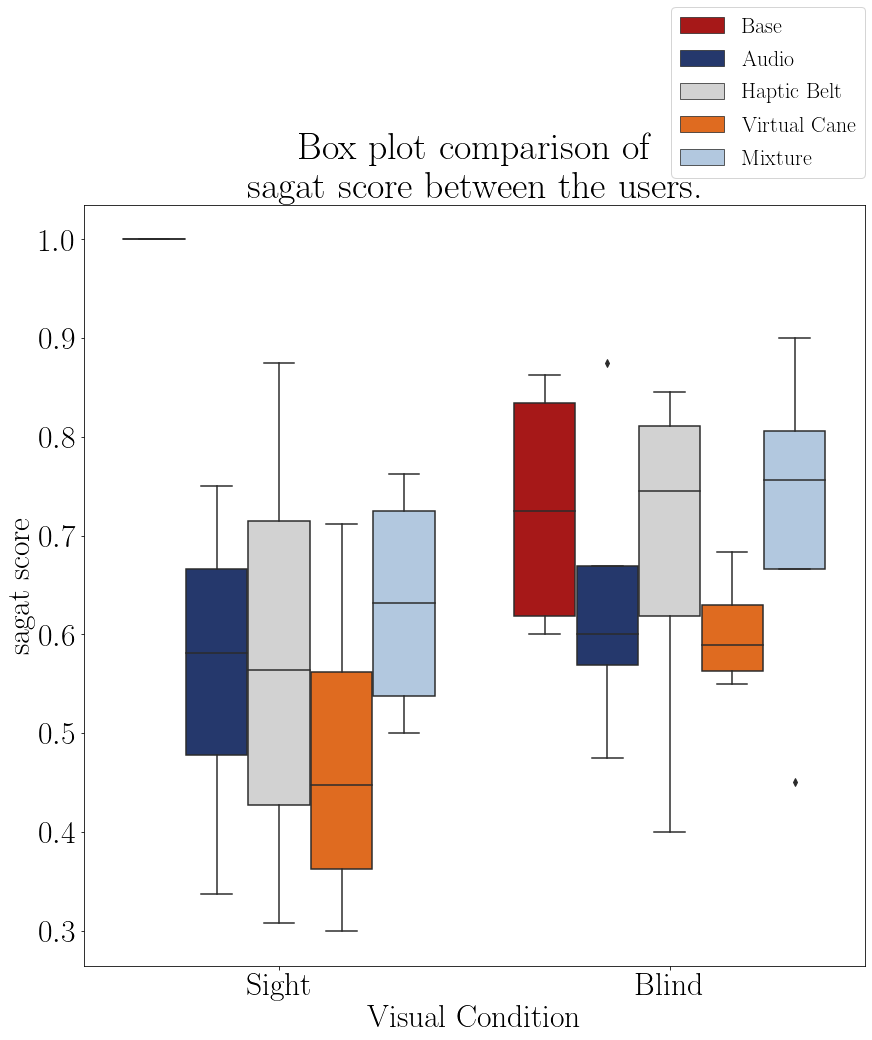
\includegraphics[width = \linewidth]{Resultados/Sagat/Figuras/png/boxplot_sagat_scene.png}
        %%% Creator: Matplotlib, PGF backend
%%
%% To include the figure in your LaTeX document, write
%%   \input{<filename>.pgf}
%%
%% Make sure the required packages are loaded in your preamble
%%   \usepackage{pgf}
%%
%% and, on pdftex
%%   \usepackage[utf8]{inputenc}\DeclareUnicodeCharacter{2212}{-}
%%
%% or, on luatex and xetex
%%   \usepackage{unicode-math}
%%
%% Figures using additional raster images can only be included by \input if
%% they are in the same directory as the main LaTeX file. For loading figures
%% from other directories you can use the `import` package
%%   \usepackage{import}
%%
%% and then include the figures with
%%   \import{<path to file>}{<filename>.pgf}
%%
%% Matplotlib used the following preamble
%%   \usepackage{url}
%%   \usepackage{unicode-math}
%%   \setmainfont{DejaVu Serif}
%%   \usepackage{fontspec}
%%
\begingroup%
\makeatletter%
\begin{pgfpicture}%
\pgfpathrectangle{\pgfpointorigin}{\pgfqpoint{12.196638in}{14.528848in}}%
\pgfusepath{use as bounding box, clip}%
\begin{pgfscope}%
\pgfsetbuttcap%
\pgfsetmiterjoin%
\pgfsetlinewidth{0.000000pt}%
\definecolor{currentstroke}{rgb}{1.000000,1.000000,1.000000}%
\pgfsetstrokecolor{currentstroke}%
\pgfsetstrokeopacity{0.000000}%
\pgfsetdash{}{0pt}%
\pgfpathmoveto{\pgfqpoint{0.000000in}{0.000000in}}%
\pgfpathlineto{\pgfqpoint{12.196638in}{0.000000in}}%
\pgfpathlineto{\pgfqpoint{12.196638in}{14.528848in}}%
\pgfpathlineto{\pgfqpoint{0.000000in}{14.528848in}}%
\pgfpathclose%
\pgfusepath{}%
\end{pgfscope}%
\begin{pgfscope}%
\pgfsetbuttcap%
\pgfsetmiterjoin%
\definecolor{currentfill}{rgb}{1.000000,1.000000,1.000000}%
\pgfsetfillcolor{currentfill}%
\pgfsetlinewidth{0.000000pt}%
\definecolor{currentstroke}{rgb}{0.000000,0.000000,0.000000}%
\pgfsetstrokecolor{currentstroke}%
\pgfsetstrokeopacity{0.000000}%
\pgfsetdash{}{0pt}%
\pgfpathmoveto{\pgfqpoint{1.246638in}{1.110648in}}%
\pgfpathlineto{\pgfqpoint{12.096638in}{1.110648in}}%
\pgfpathlineto{\pgfqpoint{12.096638in}{11.680648in}}%
\pgfpathlineto{\pgfqpoint{1.246638in}{11.680648in}}%
\pgfpathclose%
\pgfusepath{fill}%
\end{pgfscope}%
\begin{pgfscope}%
\pgfpathrectangle{\pgfqpoint{1.246638in}{1.110648in}}{\pgfqpoint{10.850000in}{10.570000in}}%
\pgfusepath{clip}%
\pgfsetbuttcap%
\pgfsetmiterjoin%
\definecolor{currentfill}{rgb}{0.651961,0.093137,0.093137}%
\pgfsetfillcolor{currentfill}%
\pgfsetlinewidth{1.505625pt}%
\definecolor{currentstroke}{rgb}{0.168627,0.168627,0.168627}%
\pgfsetstrokecolor{currentstroke}%
\pgfsetdash{}{0pt}%
\pgfpathmoveto{\pgfqpoint{1.797818in}{11.200194in}}%
\pgfpathlineto{\pgfqpoint{2.648458in}{11.200194in}}%
\pgfpathlineto{\pgfqpoint{2.648458in}{11.200194in}}%
\pgfpathlineto{\pgfqpoint{1.797818in}{11.200194in}}%
\pgfpathlineto{\pgfqpoint{1.797818in}{11.200194in}}%
\pgfpathclose%
\pgfusepath{stroke,fill}%
\end{pgfscope}%
\begin{pgfscope}%
\pgfpathrectangle{\pgfqpoint{1.246638in}{1.110648in}}{\pgfqpoint{10.850000in}{10.570000in}}%
\pgfusepath{clip}%
\pgfsetbuttcap%
\pgfsetmiterjoin%
\definecolor{currentfill}{rgb}{0.144608,0.218137,0.424020}%
\pgfsetfillcolor{currentfill}%
\pgfsetlinewidth{1.505625pt}%
\definecolor{currentstroke}{rgb}{0.168627,0.168627,0.168627}%
\pgfsetstrokecolor{currentstroke}%
\pgfsetdash{}{0pt}%
\pgfpathmoveto{\pgfqpoint{2.665818in}{4.041387in}}%
\pgfpathlineto{\pgfqpoint{3.516458in}{4.041387in}}%
\pgfpathlineto{\pgfqpoint{3.516458in}{6.613413in}}%
\pgfpathlineto{\pgfqpoint{2.665818in}{6.613413in}}%
\pgfpathlineto{\pgfqpoint{2.665818in}{4.041387in}}%
\pgfpathclose%
\pgfusepath{stroke,fill}%
\end{pgfscope}%
\begin{pgfscope}%
\pgfpathrectangle{\pgfqpoint{1.246638in}{1.110648in}}{\pgfqpoint{10.850000in}{10.570000in}}%
\pgfusepath{clip}%
\pgfsetbuttcap%
\pgfsetmiterjoin%
\definecolor{currentfill}{rgb}{0.823529,0.823529,0.823529}%
\pgfsetfillcolor{currentfill}%
\pgfsetlinewidth{1.505625pt}%
\definecolor{currentstroke}{rgb}{0.168627,0.168627,0.168627}%
\pgfsetstrokecolor{currentstroke}%
\pgfsetdash{}{0pt}%
\pgfpathmoveto{\pgfqpoint{3.533818in}{3.338366in}}%
\pgfpathlineto{\pgfqpoint{4.384458in}{3.338366in}}%
\pgfpathlineto{\pgfqpoint{4.384458in}{7.292428in}}%
\pgfpathlineto{\pgfqpoint{3.533818in}{7.292428in}}%
\pgfpathlineto{\pgfqpoint{3.533818in}{3.338366in}}%
\pgfpathclose%
\pgfusepath{stroke,fill}%
\end{pgfscope}%
\begin{pgfscope}%
\pgfpathrectangle{\pgfqpoint{1.246638in}{1.110648in}}{\pgfqpoint{10.850000in}{10.570000in}}%
\pgfusepath{clip}%
\pgfsetbuttcap%
\pgfsetmiterjoin%
\definecolor{currentfill}{rgb}{0.875000,0.419118,0.125000}%
\pgfsetfillcolor{currentfill}%
\pgfsetlinewidth{1.505625pt}%
\definecolor{currentstroke}{rgb}{0.168627,0.168627,0.168627}%
\pgfsetstrokecolor{currentstroke}%
\pgfsetdash{}{0pt}%
\pgfpathmoveto{\pgfqpoint{4.401818in}{2.450160in}}%
\pgfpathlineto{\pgfqpoint{5.252458in}{2.450160in}}%
\pgfpathlineto{\pgfqpoint{5.252458in}{5.191940in}}%
\pgfpathlineto{\pgfqpoint{4.401818in}{5.191940in}}%
\pgfpathlineto{\pgfqpoint{4.401818in}{2.450160in}}%
\pgfpathclose%
\pgfusepath{stroke,fill}%
\end{pgfscope}%
\begin{pgfscope}%
\pgfpathrectangle{\pgfqpoint{1.246638in}{1.110648in}}{\pgfqpoint{10.850000in}{10.570000in}}%
\pgfusepath{clip}%
\pgfsetbuttcap%
\pgfsetmiterjoin%
\definecolor{currentfill}{rgb}{0.696078,0.784314,0.872549}%
\pgfsetfillcolor{currentfill}%
\pgfsetlinewidth{1.505625pt}%
\definecolor{currentstroke}{rgb}{0.168627,0.168627,0.168627}%
\pgfsetstrokecolor{currentstroke}%
\pgfsetdash{}{0pt}%
\pgfpathmoveto{\pgfqpoint{5.269818in}{4.855862in}}%
\pgfpathlineto{\pgfqpoint{6.120458in}{4.855862in}}%
\pgfpathlineto{\pgfqpoint{6.120458in}{7.427888in}}%
\pgfpathlineto{\pgfqpoint{5.269818in}{7.427888in}}%
\pgfpathlineto{\pgfqpoint{5.269818in}{4.855862in}}%
\pgfpathclose%
\pgfusepath{stroke,fill}%
\end{pgfscope}%
\begin{pgfscope}%
\pgfpathrectangle{\pgfqpoint{1.246638in}{1.110648in}}{\pgfqpoint{10.850000in}{10.570000in}}%
\pgfusepath{clip}%
\pgfsetbuttcap%
\pgfsetmiterjoin%
\definecolor{currentfill}{rgb}{0.651961,0.093137,0.093137}%
\pgfsetfillcolor{currentfill}%
\pgfsetlinewidth{1.505625pt}%
\definecolor{currentstroke}{rgb}{0.168627,0.168627,0.168627}%
\pgfsetstrokecolor{currentstroke}%
\pgfsetdash{}{0pt}%
\pgfpathmoveto{\pgfqpoint{7.222818in}{5.970407in}}%
\pgfpathlineto{\pgfqpoint{8.073458in}{5.970407in}}%
\pgfpathlineto{\pgfqpoint{8.073458in}{8.928237in}}%
\pgfpathlineto{\pgfqpoint{7.222818in}{8.928237in}}%
\pgfpathlineto{\pgfqpoint{7.222818in}{5.970407in}}%
\pgfpathclose%
\pgfusepath{stroke,fill}%
\end{pgfscope}%
\begin{pgfscope}%
\pgfpathrectangle{\pgfqpoint{1.246638in}{1.110648in}}{\pgfqpoint{10.850000in}{10.570000in}}%
\pgfusepath{clip}%
\pgfsetbuttcap%
\pgfsetmiterjoin%
\definecolor{currentfill}{rgb}{0.144608,0.218137,0.424020}%
\pgfsetfillcolor{currentfill}%
\pgfsetlinewidth{1.505625pt}%
\definecolor{currentstroke}{rgb}{0.168627,0.168627,0.168627}%
\pgfsetstrokecolor{currentstroke}%
\pgfsetdash{}{0pt}%
\pgfpathmoveto{\pgfqpoint{8.090818in}{5.284533in}}%
\pgfpathlineto{\pgfqpoint{8.941458in}{5.284533in}}%
\pgfpathlineto{\pgfqpoint{8.941458in}{6.656280in}}%
\pgfpathlineto{\pgfqpoint{8.090818in}{6.656280in}}%
\pgfpathlineto{\pgfqpoint{8.090818in}{5.284533in}}%
\pgfpathclose%
\pgfusepath{stroke,fill}%
\end{pgfscope}%
\begin{pgfscope}%
\pgfpathrectangle{\pgfqpoint{1.246638in}{1.110648in}}{\pgfqpoint{10.850000in}{10.570000in}}%
\pgfusepath{clip}%
\pgfsetbuttcap%
\pgfsetmiterjoin%
\definecolor{currentfill}{rgb}{0.823529,0.823529,0.823529}%
\pgfsetfillcolor{currentfill}%
\pgfsetlinewidth{1.505625pt}%
\definecolor{currentstroke}{rgb}{0.168627,0.168627,0.168627}%
\pgfsetstrokecolor{currentstroke}%
\pgfsetdash{}{0pt}%
\pgfpathmoveto{\pgfqpoint{8.958818in}{5.966977in}}%
\pgfpathlineto{\pgfqpoint{9.809458in}{5.966977in}}%
\pgfpathlineto{\pgfqpoint{9.809458in}{8.607591in}}%
\pgfpathlineto{\pgfqpoint{8.958818in}{8.607591in}}%
\pgfpathlineto{\pgfqpoint{8.958818in}{5.966977in}}%
\pgfpathclose%
\pgfusepath{stroke,fill}%
\end{pgfscope}%
\begin{pgfscope}%
\pgfpathrectangle{\pgfqpoint{1.246638in}{1.110648in}}{\pgfqpoint{10.850000in}{10.570000in}}%
\pgfusepath{clip}%
\pgfsetbuttcap%
\pgfsetmiterjoin%
\definecolor{currentfill}{rgb}{0.875000,0.419118,0.125000}%
\pgfsetfillcolor{currentfill}%
\pgfsetlinewidth{1.505625pt}%
\definecolor{currentstroke}{rgb}{0.168627,0.168627,0.168627}%
\pgfsetstrokecolor{currentstroke}%
\pgfsetdash{}{0pt}%
\pgfpathmoveto{\pgfqpoint{9.826818in}{5.197084in}}%
\pgfpathlineto{\pgfqpoint{10.677458in}{5.197084in}}%
\pgfpathlineto{\pgfqpoint{10.677458in}{6.121299in}}%
\pgfpathlineto{\pgfqpoint{9.826818in}{6.121299in}}%
\pgfpathlineto{\pgfqpoint{9.826818in}{5.197084in}}%
\pgfpathclose%
\pgfusepath{stroke,fill}%
\end{pgfscope}%
\begin{pgfscope}%
\pgfpathrectangle{\pgfqpoint{1.246638in}{1.110648in}}{\pgfqpoint{10.850000in}{10.570000in}}%
\pgfusepath{clip}%
\pgfsetbuttcap%
\pgfsetmiterjoin%
\definecolor{currentfill}{rgb}{0.696078,0.784314,0.872549}%
\pgfsetfillcolor{currentfill}%
\pgfsetlinewidth{1.505625pt}%
\definecolor{currentstroke}{rgb}{0.168627,0.168627,0.168627}%
\pgfsetstrokecolor{currentstroke}%
\pgfsetdash{}{0pt}%
\pgfpathmoveto{\pgfqpoint{10.694818in}{6.613413in}}%
\pgfpathlineto{\pgfqpoint{11.545458in}{6.613413in}}%
\pgfpathlineto{\pgfqpoint{11.545458in}{8.542433in}}%
\pgfpathlineto{\pgfqpoint{10.694818in}{8.542433in}}%
\pgfpathlineto{\pgfqpoint{10.694818in}{6.613413in}}%
\pgfpathclose%
\pgfusepath{stroke,fill}%
\end{pgfscope}%
\begin{pgfscope}%
\pgfpathrectangle{\pgfqpoint{1.246638in}{1.110648in}}{\pgfqpoint{10.850000in}{10.570000in}}%
\pgfusepath{clip}%
\pgfsetbuttcap%
\pgfsetmiterjoin%
\definecolor{currentfill}{rgb}{0.651961,0.093137,0.093137}%
\pgfsetfillcolor{currentfill}%
\pgfsetlinewidth{0.752812pt}%
\definecolor{currentstroke}{rgb}{0.168627,0.168627,0.168627}%
\pgfsetstrokecolor{currentstroke}%
\pgfsetdash{}{0pt}%
\pgfpathmoveto{\pgfqpoint{3.959138in}{-2.517281in}}%
\pgfpathlineto{\pgfqpoint{3.959138in}{-2.517281in}}%
\pgfpathlineto{\pgfqpoint{3.959138in}{-2.517281in}}%
\pgfpathlineto{\pgfqpoint{3.959138in}{-2.517281in}}%
\pgfpathclose%
\pgfusepath{stroke,fill}%
\end{pgfscope}%
\begin{pgfscope}%
\pgfpathrectangle{\pgfqpoint{1.246638in}{1.110648in}}{\pgfqpoint{10.850000in}{10.570000in}}%
\pgfusepath{clip}%
\pgfsetbuttcap%
\pgfsetmiterjoin%
\definecolor{currentfill}{rgb}{0.144608,0.218137,0.424020}%
\pgfsetfillcolor{currentfill}%
\pgfsetlinewidth{0.752812pt}%
\definecolor{currentstroke}{rgb}{0.168627,0.168627,0.168627}%
\pgfsetstrokecolor{currentstroke}%
\pgfsetdash{}{0pt}%
\pgfpathmoveto{\pgfqpoint{3.959138in}{-2.517281in}}%
\pgfpathlineto{\pgfqpoint{3.959138in}{-2.517281in}}%
\pgfpathlineto{\pgfqpoint{3.959138in}{-2.517281in}}%
\pgfpathlineto{\pgfqpoint{3.959138in}{-2.517281in}}%
\pgfpathclose%
\pgfusepath{stroke,fill}%
\end{pgfscope}%
\begin{pgfscope}%
\pgfpathrectangle{\pgfqpoint{1.246638in}{1.110648in}}{\pgfqpoint{10.850000in}{10.570000in}}%
\pgfusepath{clip}%
\pgfsetbuttcap%
\pgfsetmiterjoin%
\definecolor{currentfill}{rgb}{0.823529,0.823529,0.823529}%
\pgfsetfillcolor{currentfill}%
\pgfsetlinewidth{0.752812pt}%
\definecolor{currentstroke}{rgb}{0.168627,0.168627,0.168627}%
\pgfsetstrokecolor{currentstroke}%
\pgfsetdash{}{0pt}%
\pgfpathmoveto{\pgfqpoint{3.959138in}{-2.517281in}}%
\pgfpathlineto{\pgfqpoint{3.959138in}{-2.517281in}}%
\pgfpathlineto{\pgfqpoint{3.959138in}{-2.517281in}}%
\pgfpathlineto{\pgfqpoint{3.959138in}{-2.517281in}}%
\pgfpathclose%
\pgfusepath{stroke,fill}%
\end{pgfscope}%
\begin{pgfscope}%
\pgfpathrectangle{\pgfqpoint{1.246638in}{1.110648in}}{\pgfqpoint{10.850000in}{10.570000in}}%
\pgfusepath{clip}%
\pgfsetbuttcap%
\pgfsetmiterjoin%
\definecolor{currentfill}{rgb}{0.875000,0.419118,0.125000}%
\pgfsetfillcolor{currentfill}%
\pgfsetlinewidth{0.752812pt}%
\definecolor{currentstroke}{rgb}{0.168627,0.168627,0.168627}%
\pgfsetstrokecolor{currentstroke}%
\pgfsetdash{}{0pt}%
\pgfpathmoveto{\pgfqpoint{3.959138in}{-2.517281in}}%
\pgfpathlineto{\pgfqpoint{3.959138in}{-2.517281in}}%
\pgfpathlineto{\pgfqpoint{3.959138in}{-2.517281in}}%
\pgfpathlineto{\pgfqpoint{3.959138in}{-2.517281in}}%
\pgfpathclose%
\pgfusepath{stroke,fill}%
\end{pgfscope}%
\begin{pgfscope}%
\pgfpathrectangle{\pgfqpoint{1.246638in}{1.110648in}}{\pgfqpoint{10.850000in}{10.570000in}}%
\pgfusepath{clip}%
\pgfsetbuttcap%
\pgfsetmiterjoin%
\definecolor{currentfill}{rgb}{0.696078,0.784314,0.872549}%
\pgfsetfillcolor{currentfill}%
\pgfsetlinewidth{0.752812pt}%
\definecolor{currentstroke}{rgb}{0.168627,0.168627,0.168627}%
\pgfsetstrokecolor{currentstroke}%
\pgfsetdash{}{0pt}%
\pgfpathmoveto{\pgfqpoint{3.959138in}{-2.517281in}}%
\pgfpathlineto{\pgfqpoint{3.959138in}{-2.517281in}}%
\pgfpathlineto{\pgfqpoint{3.959138in}{-2.517281in}}%
\pgfpathlineto{\pgfqpoint{3.959138in}{-2.517281in}}%
\pgfpathclose%
\pgfusepath{stroke,fill}%
\end{pgfscope}%
\begin{pgfscope}%
\pgfsetbuttcap%
\pgfsetroundjoin%
\definecolor{currentfill}{rgb}{0.000000,0.000000,0.000000}%
\pgfsetfillcolor{currentfill}%
\pgfsetlinewidth{0.803000pt}%
\definecolor{currentstroke}{rgb}{0.000000,0.000000,0.000000}%
\pgfsetstrokecolor{currentstroke}%
\pgfsetdash{}{0pt}%
\pgfsys@defobject{currentmarker}{\pgfqpoint{0.000000in}{-0.048611in}}{\pgfqpoint{0.000000in}{0.000000in}}{%
\pgfpathmoveto{\pgfqpoint{0.000000in}{0.000000in}}%
\pgfpathlineto{\pgfqpoint{0.000000in}{-0.048611in}}%
\pgfusepath{stroke,fill}%
}%
\begin{pgfscope}%
\pgfsys@transformshift{3.959138in}{1.110648in}%
\pgfsys@useobject{currentmarker}{}%
\end{pgfscope}%
\end{pgfscope}%
\begin{pgfscope}%
\definecolor{textcolor}{rgb}{0.000000,0.000000,0.000000}%
\pgfsetstrokecolor{textcolor}%
\pgfsetfillcolor{textcolor}%
\pgftext[x=3.959138in,y=1.013426in,,top]{\color{textcolor}\rmfamily\fontsize{31.680000}{38.016000}\selectfont Sight}%
\end{pgfscope}%
\begin{pgfscope}%
\pgfsetbuttcap%
\pgfsetroundjoin%
\definecolor{currentfill}{rgb}{0.000000,0.000000,0.000000}%
\pgfsetfillcolor{currentfill}%
\pgfsetlinewidth{0.803000pt}%
\definecolor{currentstroke}{rgb}{0.000000,0.000000,0.000000}%
\pgfsetstrokecolor{currentstroke}%
\pgfsetdash{}{0pt}%
\pgfsys@defobject{currentmarker}{\pgfqpoint{0.000000in}{-0.048611in}}{\pgfqpoint{0.000000in}{0.000000in}}{%
\pgfpathmoveto{\pgfqpoint{0.000000in}{0.000000in}}%
\pgfpathlineto{\pgfqpoint{0.000000in}{-0.048611in}}%
\pgfusepath{stroke,fill}%
}%
\begin{pgfscope}%
\pgfsys@transformshift{9.384138in}{1.110648in}%
\pgfsys@useobject{currentmarker}{}%
\end{pgfscope}%
\end{pgfscope}%
\begin{pgfscope}%
\definecolor{textcolor}{rgb}{0.000000,0.000000,0.000000}%
\pgfsetstrokecolor{textcolor}%
\pgfsetfillcolor{textcolor}%
\pgftext[x=9.384138in,y=1.013426in,,top]{\color{textcolor}\rmfamily\fontsize{31.680000}{38.016000}\selectfont Blind}%
\end{pgfscope}%
\begin{pgfscope}%
\definecolor{textcolor}{rgb}{0.000000,0.000000,0.000000}%
\pgfsetstrokecolor{textcolor}%
\pgfsetfillcolor{textcolor}%
\pgftext[x=6.671638in,y=0.525820in,,top]{\color{textcolor}\rmfamily\fontsize{31.680000}{38.016000}\selectfont Visual Condition}%
\end{pgfscope}%
\begin{pgfscope}%
\pgfsetbuttcap%
\pgfsetroundjoin%
\definecolor{currentfill}{rgb}{0.000000,0.000000,0.000000}%
\pgfsetfillcolor{currentfill}%
\pgfsetlinewidth{0.803000pt}%
\definecolor{currentstroke}{rgb}{0.000000,0.000000,0.000000}%
\pgfsetstrokecolor{currentstroke}%
\pgfsetdash{}{0pt}%
\pgfsys@defobject{currentmarker}{\pgfqpoint{-0.048611in}{0.000000in}}{\pgfqpoint{-0.000000in}{0.000000in}}{%
\pgfpathmoveto{\pgfqpoint{-0.000000in}{0.000000in}}%
\pgfpathlineto{\pgfqpoint{-0.048611in}{0.000000in}}%
\pgfusepath{stroke,fill}%
}%
\begin{pgfscope}%
\pgfsys@transformshift{1.246638in}{1.597962in}%
\pgfsys@useobject{currentmarker}{}%
\end{pgfscope}%
\end{pgfscope}%
\begin{pgfscope}%
\definecolor{textcolor}{rgb}{0.000000,0.000000,0.000000}%
\pgfsetstrokecolor{textcolor}%
\pgfsetfillcolor{textcolor}%
\pgftext[x=0.587096in, y=1.430813in, left, base]{\color{textcolor}\rmfamily\fontsize{31.680000}{38.016000}\selectfont \(\displaystyle {0.3}\)}%
\end{pgfscope}%
\begin{pgfscope}%
\pgfsetbuttcap%
\pgfsetroundjoin%
\definecolor{currentfill}{rgb}{0.000000,0.000000,0.000000}%
\pgfsetfillcolor{currentfill}%
\pgfsetlinewidth{0.803000pt}%
\definecolor{currentstroke}{rgb}{0.000000,0.000000,0.000000}%
\pgfsetstrokecolor{currentstroke}%
\pgfsetdash{}{0pt}%
\pgfsys@defobject{currentmarker}{\pgfqpoint{-0.048611in}{0.000000in}}{\pgfqpoint{-0.000000in}{0.000000in}}{%
\pgfpathmoveto{\pgfqpoint{-0.000000in}{0.000000in}}%
\pgfpathlineto{\pgfqpoint{-0.048611in}{0.000000in}}%
\pgfusepath{stroke,fill}%
}%
\begin{pgfscope}%
\pgfsys@transformshift{1.246638in}{2.969709in}%
\pgfsys@useobject{currentmarker}{}%
\end{pgfscope}%
\end{pgfscope}%
\begin{pgfscope}%
\definecolor{textcolor}{rgb}{0.000000,0.000000,0.000000}%
\pgfsetstrokecolor{textcolor}%
\pgfsetfillcolor{textcolor}%
\pgftext[x=0.587096in, y=2.802561in, left, base]{\color{textcolor}\rmfamily\fontsize{31.680000}{38.016000}\selectfont \(\displaystyle {0.4}\)}%
\end{pgfscope}%
\begin{pgfscope}%
\pgfsetbuttcap%
\pgfsetroundjoin%
\definecolor{currentfill}{rgb}{0.000000,0.000000,0.000000}%
\pgfsetfillcolor{currentfill}%
\pgfsetlinewidth{0.803000pt}%
\definecolor{currentstroke}{rgb}{0.000000,0.000000,0.000000}%
\pgfsetstrokecolor{currentstroke}%
\pgfsetdash{}{0pt}%
\pgfsys@defobject{currentmarker}{\pgfqpoint{-0.048611in}{0.000000in}}{\pgfqpoint{-0.000000in}{0.000000in}}{%
\pgfpathmoveto{\pgfqpoint{-0.000000in}{0.000000in}}%
\pgfpathlineto{\pgfqpoint{-0.048611in}{0.000000in}}%
\pgfusepath{stroke,fill}%
}%
\begin{pgfscope}%
\pgfsys@transformshift{1.246638in}{4.341457in}%
\pgfsys@useobject{currentmarker}{}%
\end{pgfscope}%
\end{pgfscope}%
\begin{pgfscope}%
\definecolor{textcolor}{rgb}{0.000000,0.000000,0.000000}%
\pgfsetstrokecolor{textcolor}%
\pgfsetfillcolor{textcolor}%
\pgftext[x=0.587096in, y=4.174308in, left, base]{\color{textcolor}\rmfamily\fontsize{31.680000}{38.016000}\selectfont \(\displaystyle {0.5}\)}%
\end{pgfscope}%
\begin{pgfscope}%
\pgfsetbuttcap%
\pgfsetroundjoin%
\definecolor{currentfill}{rgb}{0.000000,0.000000,0.000000}%
\pgfsetfillcolor{currentfill}%
\pgfsetlinewidth{0.803000pt}%
\definecolor{currentstroke}{rgb}{0.000000,0.000000,0.000000}%
\pgfsetstrokecolor{currentstroke}%
\pgfsetdash{}{0pt}%
\pgfsys@defobject{currentmarker}{\pgfqpoint{-0.048611in}{0.000000in}}{\pgfqpoint{-0.000000in}{0.000000in}}{%
\pgfpathmoveto{\pgfqpoint{-0.000000in}{0.000000in}}%
\pgfpathlineto{\pgfqpoint{-0.048611in}{0.000000in}}%
\pgfusepath{stroke,fill}%
}%
\begin{pgfscope}%
\pgfsys@transformshift{1.246638in}{5.713204in}%
\pgfsys@useobject{currentmarker}{}%
\end{pgfscope}%
\end{pgfscope}%
\begin{pgfscope}%
\definecolor{textcolor}{rgb}{0.000000,0.000000,0.000000}%
\pgfsetstrokecolor{textcolor}%
\pgfsetfillcolor{textcolor}%
\pgftext[x=0.587096in, y=5.546056in, left, base]{\color{textcolor}\rmfamily\fontsize{31.680000}{38.016000}\selectfont \(\displaystyle {0.6}\)}%
\end{pgfscope}%
\begin{pgfscope}%
\pgfsetbuttcap%
\pgfsetroundjoin%
\definecolor{currentfill}{rgb}{0.000000,0.000000,0.000000}%
\pgfsetfillcolor{currentfill}%
\pgfsetlinewidth{0.803000pt}%
\definecolor{currentstroke}{rgb}{0.000000,0.000000,0.000000}%
\pgfsetstrokecolor{currentstroke}%
\pgfsetdash{}{0pt}%
\pgfsys@defobject{currentmarker}{\pgfqpoint{-0.048611in}{0.000000in}}{\pgfqpoint{-0.000000in}{0.000000in}}{%
\pgfpathmoveto{\pgfqpoint{-0.000000in}{0.000000in}}%
\pgfpathlineto{\pgfqpoint{-0.048611in}{0.000000in}}%
\pgfusepath{stroke,fill}%
}%
\begin{pgfscope}%
\pgfsys@transformshift{1.246638in}{7.084952in}%
\pgfsys@useobject{currentmarker}{}%
\end{pgfscope}%
\end{pgfscope}%
\begin{pgfscope}%
\definecolor{textcolor}{rgb}{0.000000,0.000000,0.000000}%
\pgfsetstrokecolor{textcolor}%
\pgfsetfillcolor{textcolor}%
\pgftext[x=0.581376in, y=6.917803in, left, base]{\color{textcolor}\rmfamily\fontsize{31.680000}{38.016000}\selectfont \(\displaystyle {0.7}\)}%
\end{pgfscope}%
\begin{pgfscope}%
\pgfsetbuttcap%
\pgfsetroundjoin%
\definecolor{currentfill}{rgb}{0.000000,0.000000,0.000000}%
\pgfsetfillcolor{currentfill}%
\pgfsetlinewidth{0.803000pt}%
\definecolor{currentstroke}{rgb}{0.000000,0.000000,0.000000}%
\pgfsetstrokecolor{currentstroke}%
\pgfsetdash{}{0pt}%
\pgfsys@defobject{currentmarker}{\pgfqpoint{-0.048611in}{0.000000in}}{\pgfqpoint{-0.000000in}{0.000000in}}{%
\pgfpathmoveto{\pgfqpoint{-0.000000in}{0.000000in}}%
\pgfpathlineto{\pgfqpoint{-0.048611in}{0.000000in}}%
\pgfusepath{stroke,fill}%
}%
\begin{pgfscope}%
\pgfsys@transformshift{1.246638in}{8.456699in}%
\pgfsys@useobject{currentmarker}{}%
\end{pgfscope}%
\end{pgfscope}%
\begin{pgfscope}%
\definecolor{textcolor}{rgb}{0.000000,0.000000,0.000000}%
\pgfsetstrokecolor{textcolor}%
\pgfsetfillcolor{textcolor}%
\pgftext[x=0.587096in, y=8.289551in, left, base]{\color{textcolor}\rmfamily\fontsize{31.680000}{38.016000}\selectfont \(\displaystyle {0.8}\)}%
\end{pgfscope}%
\begin{pgfscope}%
\pgfsetbuttcap%
\pgfsetroundjoin%
\definecolor{currentfill}{rgb}{0.000000,0.000000,0.000000}%
\pgfsetfillcolor{currentfill}%
\pgfsetlinewidth{0.803000pt}%
\definecolor{currentstroke}{rgb}{0.000000,0.000000,0.000000}%
\pgfsetstrokecolor{currentstroke}%
\pgfsetdash{}{0pt}%
\pgfsys@defobject{currentmarker}{\pgfqpoint{-0.048611in}{0.000000in}}{\pgfqpoint{-0.000000in}{0.000000in}}{%
\pgfpathmoveto{\pgfqpoint{-0.000000in}{0.000000in}}%
\pgfpathlineto{\pgfqpoint{-0.048611in}{0.000000in}}%
\pgfusepath{stroke,fill}%
}%
\begin{pgfscope}%
\pgfsys@transformshift{1.246638in}{9.828446in}%
\pgfsys@useobject{currentmarker}{}%
\end{pgfscope}%
\end{pgfscope}%
\begin{pgfscope}%
\definecolor{textcolor}{rgb}{0.000000,0.000000,0.000000}%
\pgfsetstrokecolor{textcolor}%
\pgfsetfillcolor{textcolor}%
\pgftext[x=0.587096in, y=9.661298in, left, base]{\color{textcolor}\rmfamily\fontsize{31.680000}{38.016000}\selectfont \(\displaystyle {0.9}\)}%
\end{pgfscope}%
\begin{pgfscope}%
\pgfsetbuttcap%
\pgfsetroundjoin%
\definecolor{currentfill}{rgb}{0.000000,0.000000,0.000000}%
\pgfsetfillcolor{currentfill}%
\pgfsetlinewidth{0.803000pt}%
\definecolor{currentstroke}{rgb}{0.000000,0.000000,0.000000}%
\pgfsetstrokecolor{currentstroke}%
\pgfsetdash{}{0pt}%
\pgfsys@defobject{currentmarker}{\pgfqpoint{-0.048611in}{0.000000in}}{\pgfqpoint{-0.000000in}{0.000000in}}{%
\pgfpathmoveto{\pgfqpoint{-0.000000in}{0.000000in}}%
\pgfpathlineto{\pgfqpoint{-0.048611in}{0.000000in}}%
\pgfusepath{stroke,fill}%
}%
\begin{pgfscope}%
\pgfsys@transformshift{1.246638in}{11.200194in}%
\pgfsys@useobject{currentmarker}{}%
\end{pgfscope}%
\end{pgfscope}%
\begin{pgfscope}%
\definecolor{textcolor}{rgb}{0.000000,0.000000,0.000000}%
\pgfsetstrokecolor{textcolor}%
\pgfsetfillcolor{textcolor}%
\pgftext[x=0.587096in, y=11.033046in, left, base]{\color{textcolor}\rmfamily\fontsize{31.680000}{38.016000}\selectfont \(\displaystyle {1.0}\)}%
\end{pgfscope}%
\begin{pgfscope}%
\definecolor{textcolor}{rgb}{0.000000,0.000000,0.000000}%
\pgfsetstrokecolor{textcolor}%
\pgfsetfillcolor{textcolor}%
\pgftext[x=0.525820in,y=6.395648in,,bottom,rotate=90.000000]{\color{textcolor}\rmfamily\fontsize{31.680000}{38.016000}\selectfont sagat score}%
\end{pgfscope}%
\begin{pgfscope}%
\pgfpathrectangle{\pgfqpoint{1.246638in}{1.110648in}}{\pgfqpoint{10.850000in}{10.570000in}}%
\pgfusepath{clip}%
\pgfsetrectcap%
\pgfsetroundjoin%
\pgfsetlinewidth{1.505625pt}%
\definecolor{currentstroke}{rgb}{0.168627,0.168627,0.168627}%
\pgfsetstrokecolor{currentstroke}%
\pgfsetdash{}{0pt}%
\pgfpathmoveto{\pgfqpoint{2.223138in}{11.200194in}}%
\pgfpathlineto{\pgfqpoint{2.223138in}{11.200194in}}%
\pgfusepath{stroke}%
\end{pgfscope}%
\begin{pgfscope}%
\pgfpathrectangle{\pgfqpoint{1.246638in}{1.110648in}}{\pgfqpoint{10.850000in}{10.570000in}}%
\pgfusepath{clip}%
\pgfsetrectcap%
\pgfsetroundjoin%
\pgfsetlinewidth{1.505625pt}%
\definecolor{currentstroke}{rgb}{0.168627,0.168627,0.168627}%
\pgfsetstrokecolor{currentstroke}%
\pgfsetdash{}{0pt}%
\pgfpathmoveto{\pgfqpoint{2.223138in}{11.200194in}}%
\pgfpathlineto{\pgfqpoint{2.223138in}{11.200194in}}%
\pgfusepath{stroke}%
\end{pgfscope}%
\begin{pgfscope}%
\pgfpathrectangle{\pgfqpoint{1.246638in}{1.110648in}}{\pgfqpoint{10.850000in}{10.570000in}}%
\pgfusepath{clip}%
\pgfsetrectcap%
\pgfsetroundjoin%
\pgfsetlinewidth{1.505625pt}%
\definecolor{currentstroke}{rgb}{0.168627,0.168627,0.168627}%
\pgfsetstrokecolor{currentstroke}%
\pgfsetdash{}{0pt}%
\pgfpathmoveto{\pgfqpoint{2.010478in}{11.200194in}}%
\pgfpathlineto{\pgfqpoint{2.435798in}{11.200194in}}%
\pgfusepath{stroke}%
\end{pgfscope}%
\begin{pgfscope}%
\pgfpathrectangle{\pgfqpoint{1.246638in}{1.110648in}}{\pgfqpoint{10.850000in}{10.570000in}}%
\pgfusepath{clip}%
\pgfsetrectcap%
\pgfsetroundjoin%
\pgfsetlinewidth{1.505625pt}%
\definecolor{currentstroke}{rgb}{0.168627,0.168627,0.168627}%
\pgfsetstrokecolor{currentstroke}%
\pgfsetdash{}{0pt}%
\pgfpathmoveto{\pgfqpoint{2.010478in}{11.200194in}}%
\pgfpathlineto{\pgfqpoint{2.435798in}{11.200194in}}%
\pgfusepath{stroke}%
\end{pgfscope}%
\begin{pgfscope}%
\pgfpathrectangle{\pgfqpoint{1.246638in}{1.110648in}}{\pgfqpoint{10.850000in}{10.570000in}}%
\pgfusepath{clip}%
\pgfsetrectcap%
\pgfsetroundjoin%
\pgfsetlinewidth{1.505625pt}%
\definecolor{currentstroke}{rgb}{0.168627,0.168627,0.168627}%
\pgfsetstrokecolor{currentstroke}%
\pgfsetdash{}{0pt}%
\pgfpathmoveto{\pgfqpoint{3.091138in}{4.041387in}}%
\pgfpathlineto{\pgfqpoint{3.091138in}{2.112367in}}%
\pgfusepath{stroke}%
\end{pgfscope}%
\begin{pgfscope}%
\pgfpathrectangle{\pgfqpoint{1.246638in}{1.110648in}}{\pgfqpoint{10.850000in}{10.570000in}}%
\pgfusepath{clip}%
\pgfsetrectcap%
\pgfsetroundjoin%
\pgfsetlinewidth{1.505625pt}%
\definecolor{currentstroke}{rgb}{0.168627,0.168627,0.168627}%
\pgfsetstrokecolor{currentstroke}%
\pgfsetdash{}{0pt}%
\pgfpathmoveto{\pgfqpoint{3.091138in}{6.613413in}}%
\pgfpathlineto{\pgfqpoint{3.091138in}{7.770825in}}%
\pgfusepath{stroke}%
\end{pgfscope}%
\begin{pgfscope}%
\pgfpathrectangle{\pgfqpoint{1.246638in}{1.110648in}}{\pgfqpoint{10.850000in}{10.570000in}}%
\pgfusepath{clip}%
\pgfsetrectcap%
\pgfsetroundjoin%
\pgfsetlinewidth{1.505625pt}%
\definecolor{currentstroke}{rgb}{0.168627,0.168627,0.168627}%
\pgfsetstrokecolor{currentstroke}%
\pgfsetdash{}{0pt}%
\pgfpathmoveto{\pgfqpoint{2.878478in}{2.112367in}}%
\pgfpathlineto{\pgfqpoint{3.303798in}{2.112367in}}%
\pgfusepath{stroke}%
\end{pgfscope}%
\begin{pgfscope}%
\pgfpathrectangle{\pgfqpoint{1.246638in}{1.110648in}}{\pgfqpoint{10.850000in}{10.570000in}}%
\pgfusepath{clip}%
\pgfsetrectcap%
\pgfsetroundjoin%
\pgfsetlinewidth{1.505625pt}%
\definecolor{currentstroke}{rgb}{0.168627,0.168627,0.168627}%
\pgfsetstrokecolor{currentstroke}%
\pgfsetdash{}{0pt}%
\pgfpathmoveto{\pgfqpoint{2.878478in}{7.770825in}}%
\pgfpathlineto{\pgfqpoint{3.303798in}{7.770825in}}%
\pgfusepath{stroke}%
\end{pgfscope}%
\begin{pgfscope}%
\pgfpathrectangle{\pgfqpoint{1.246638in}{1.110648in}}{\pgfqpoint{10.850000in}{10.570000in}}%
\pgfusepath{clip}%
\pgfsetrectcap%
\pgfsetroundjoin%
\pgfsetlinewidth{1.505625pt}%
\definecolor{currentstroke}{rgb}{0.168627,0.168627,0.168627}%
\pgfsetstrokecolor{currentstroke}%
\pgfsetdash{}{0pt}%
\pgfpathmoveto{\pgfqpoint{3.959138in}{3.338366in}}%
\pgfpathlineto{\pgfqpoint{3.959138in}{1.707702in}}%
\pgfusepath{stroke}%
\end{pgfscope}%
\begin{pgfscope}%
\pgfpathrectangle{\pgfqpoint{1.246638in}{1.110648in}}{\pgfqpoint{10.850000in}{10.570000in}}%
\pgfusepath{clip}%
\pgfsetrectcap%
\pgfsetroundjoin%
\pgfsetlinewidth{1.505625pt}%
\definecolor{currentstroke}{rgb}{0.168627,0.168627,0.168627}%
\pgfsetstrokecolor{currentstroke}%
\pgfsetdash{}{0pt}%
\pgfpathmoveto{\pgfqpoint{3.959138in}{7.292428in}}%
\pgfpathlineto{\pgfqpoint{3.959138in}{9.478651in}}%
\pgfusepath{stroke}%
\end{pgfscope}%
\begin{pgfscope}%
\pgfpathrectangle{\pgfqpoint{1.246638in}{1.110648in}}{\pgfqpoint{10.850000in}{10.570000in}}%
\pgfusepath{clip}%
\pgfsetrectcap%
\pgfsetroundjoin%
\pgfsetlinewidth{1.505625pt}%
\definecolor{currentstroke}{rgb}{0.168627,0.168627,0.168627}%
\pgfsetstrokecolor{currentstroke}%
\pgfsetdash{}{0pt}%
\pgfpathmoveto{\pgfqpoint{3.746478in}{1.707702in}}%
\pgfpathlineto{\pgfqpoint{4.171798in}{1.707702in}}%
\pgfusepath{stroke}%
\end{pgfscope}%
\begin{pgfscope}%
\pgfpathrectangle{\pgfqpoint{1.246638in}{1.110648in}}{\pgfqpoint{10.850000in}{10.570000in}}%
\pgfusepath{clip}%
\pgfsetrectcap%
\pgfsetroundjoin%
\pgfsetlinewidth{1.505625pt}%
\definecolor{currentstroke}{rgb}{0.168627,0.168627,0.168627}%
\pgfsetstrokecolor{currentstroke}%
\pgfsetdash{}{0pt}%
\pgfpathmoveto{\pgfqpoint{3.746478in}{9.478651in}}%
\pgfpathlineto{\pgfqpoint{4.171798in}{9.478651in}}%
\pgfusepath{stroke}%
\end{pgfscope}%
\begin{pgfscope}%
\pgfpathrectangle{\pgfqpoint{1.246638in}{1.110648in}}{\pgfqpoint{10.850000in}{10.570000in}}%
\pgfusepath{clip}%
\pgfsetrectcap%
\pgfsetroundjoin%
\pgfsetlinewidth{1.505625pt}%
\definecolor{currentstroke}{rgb}{0.168627,0.168627,0.168627}%
\pgfsetstrokecolor{currentstroke}%
\pgfsetdash{}{0pt}%
\pgfpathmoveto{\pgfqpoint{4.827138in}{2.450160in}}%
\pgfpathlineto{\pgfqpoint{4.827138in}{1.591103in}}%
\pgfusepath{stroke}%
\end{pgfscope}%
\begin{pgfscope}%
\pgfpathrectangle{\pgfqpoint{1.246638in}{1.110648in}}{\pgfqpoint{10.850000in}{10.570000in}}%
\pgfusepath{clip}%
\pgfsetrectcap%
\pgfsetroundjoin%
\pgfsetlinewidth{1.505625pt}%
\definecolor{currentstroke}{rgb}{0.168627,0.168627,0.168627}%
\pgfsetstrokecolor{currentstroke}%
\pgfsetdash{}{0pt}%
\pgfpathmoveto{\pgfqpoint{4.827138in}{5.191940in}}%
\pgfpathlineto{\pgfqpoint{4.827138in}{7.249561in}}%
\pgfusepath{stroke}%
\end{pgfscope}%
\begin{pgfscope}%
\pgfpathrectangle{\pgfqpoint{1.246638in}{1.110648in}}{\pgfqpoint{10.850000in}{10.570000in}}%
\pgfusepath{clip}%
\pgfsetrectcap%
\pgfsetroundjoin%
\pgfsetlinewidth{1.505625pt}%
\definecolor{currentstroke}{rgb}{0.168627,0.168627,0.168627}%
\pgfsetstrokecolor{currentstroke}%
\pgfsetdash{}{0pt}%
\pgfpathmoveto{\pgfqpoint{4.614478in}{1.591103in}}%
\pgfpathlineto{\pgfqpoint{5.039798in}{1.591103in}}%
\pgfusepath{stroke}%
\end{pgfscope}%
\begin{pgfscope}%
\pgfpathrectangle{\pgfqpoint{1.246638in}{1.110648in}}{\pgfqpoint{10.850000in}{10.570000in}}%
\pgfusepath{clip}%
\pgfsetrectcap%
\pgfsetroundjoin%
\pgfsetlinewidth{1.505625pt}%
\definecolor{currentstroke}{rgb}{0.168627,0.168627,0.168627}%
\pgfsetstrokecolor{currentstroke}%
\pgfsetdash{}{0pt}%
\pgfpathmoveto{\pgfqpoint{4.614478in}{7.249561in}}%
\pgfpathlineto{\pgfqpoint{5.039798in}{7.249561in}}%
\pgfusepath{stroke}%
\end{pgfscope}%
\begin{pgfscope}%
\pgfpathrectangle{\pgfqpoint{1.246638in}{1.110648in}}{\pgfqpoint{10.850000in}{10.570000in}}%
\pgfusepath{clip}%
\pgfsetrectcap%
\pgfsetroundjoin%
\pgfsetlinewidth{1.505625pt}%
\definecolor{currentstroke}{rgb}{0.168627,0.168627,0.168627}%
\pgfsetstrokecolor{currentstroke}%
\pgfsetdash{}{0pt}%
\pgfpathmoveto{\pgfqpoint{5.695138in}{4.855862in}}%
\pgfpathlineto{\pgfqpoint{5.695138in}{4.341457in}}%
\pgfusepath{stroke}%
\end{pgfscope}%
\begin{pgfscope}%
\pgfpathrectangle{\pgfqpoint{1.246638in}{1.110648in}}{\pgfqpoint{10.850000in}{10.570000in}}%
\pgfusepath{clip}%
\pgfsetrectcap%
\pgfsetroundjoin%
\pgfsetlinewidth{1.505625pt}%
\definecolor{currentstroke}{rgb}{0.168627,0.168627,0.168627}%
\pgfsetstrokecolor{currentstroke}%
\pgfsetdash{}{0pt}%
\pgfpathmoveto{\pgfqpoint{5.695138in}{7.427888in}}%
\pgfpathlineto{\pgfqpoint{5.695138in}{7.942294in}}%
\pgfusepath{stroke}%
\end{pgfscope}%
\begin{pgfscope}%
\pgfpathrectangle{\pgfqpoint{1.246638in}{1.110648in}}{\pgfqpoint{10.850000in}{10.570000in}}%
\pgfusepath{clip}%
\pgfsetrectcap%
\pgfsetroundjoin%
\pgfsetlinewidth{1.505625pt}%
\definecolor{currentstroke}{rgb}{0.168627,0.168627,0.168627}%
\pgfsetstrokecolor{currentstroke}%
\pgfsetdash{}{0pt}%
\pgfpathmoveto{\pgfqpoint{5.482478in}{4.341457in}}%
\pgfpathlineto{\pgfqpoint{5.907798in}{4.341457in}}%
\pgfusepath{stroke}%
\end{pgfscope}%
\begin{pgfscope}%
\pgfpathrectangle{\pgfqpoint{1.246638in}{1.110648in}}{\pgfqpoint{10.850000in}{10.570000in}}%
\pgfusepath{clip}%
\pgfsetrectcap%
\pgfsetroundjoin%
\pgfsetlinewidth{1.505625pt}%
\definecolor{currentstroke}{rgb}{0.168627,0.168627,0.168627}%
\pgfsetstrokecolor{currentstroke}%
\pgfsetdash{}{0pt}%
\pgfpathmoveto{\pgfqpoint{5.482478in}{7.942294in}}%
\pgfpathlineto{\pgfqpoint{5.907798in}{7.942294in}}%
\pgfusepath{stroke}%
\end{pgfscope}%
\begin{pgfscope}%
\pgfpathrectangle{\pgfqpoint{1.246638in}{1.110648in}}{\pgfqpoint{10.850000in}{10.570000in}}%
\pgfusepath{clip}%
\pgfsetrectcap%
\pgfsetroundjoin%
\pgfsetlinewidth{1.505625pt}%
\definecolor{currentstroke}{rgb}{0.168627,0.168627,0.168627}%
\pgfsetstrokecolor{currentstroke}%
\pgfsetdash{}{0pt}%
\pgfpathmoveto{\pgfqpoint{7.648138in}{5.970407in}}%
\pgfpathlineto{\pgfqpoint{7.648138in}{5.713204in}}%
\pgfusepath{stroke}%
\end{pgfscope}%
\begin{pgfscope}%
\pgfpathrectangle{\pgfqpoint{1.246638in}{1.110648in}}{\pgfqpoint{10.850000in}{10.570000in}}%
\pgfusepath{clip}%
\pgfsetrectcap%
\pgfsetroundjoin%
\pgfsetlinewidth{1.505625pt}%
\definecolor{currentstroke}{rgb}{0.168627,0.168627,0.168627}%
\pgfsetstrokecolor{currentstroke}%
\pgfsetdash{}{0pt}%
\pgfpathmoveto{\pgfqpoint{7.648138in}{8.928237in}}%
\pgfpathlineto{\pgfqpoint{7.648138in}{9.314041in}}%
\pgfusepath{stroke}%
\end{pgfscope}%
\begin{pgfscope}%
\pgfpathrectangle{\pgfqpoint{1.246638in}{1.110648in}}{\pgfqpoint{10.850000in}{10.570000in}}%
\pgfusepath{clip}%
\pgfsetrectcap%
\pgfsetroundjoin%
\pgfsetlinewidth{1.505625pt}%
\definecolor{currentstroke}{rgb}{0.168627,0.168627,0.168627}%
\pgfsetstrokecolor{currentstroke}%
\pgfsetdash{}{0pt}%
\pgfpathmoveto{\pgfqpoint{7.435478in}{5.713204in}}%
\pgfpathlineto{\pgfqpoint{7.860798in}{5.713204in}}%
\pgfusepath{stroke}%
\end{pgfscope}%
\begin{pgfscope}%
\pgfpathrectangle{\pgfqpoint{1.246638in}{1.110648in}}{\pgfqpoint{10.850000in}{10.570000in}}%
\pgfusepath{clip}%
\pgfsetrectcap%
\pgfsetroundjoin%
\pgfsetlinewidth{1.505625pt}%
\definecolor{currentstroke}{rgb}{0.168627,0.168627,0.168627}%
\pgfsetstrokecolor{currentstroke}%
\pgfsetdash{}{0pt}%
\pgfpathmoveto{\pgfqpoint{7.435478in}{9.314041in}}%
\pgfpathlineto{\pgfqpoint{7.860798in}{9.314041in}}%
\pgfusepath{stroke}%
\end{pgfscope}%
\begin{pgfscope}%
\pgfpathrectangle{\pgfqpoint{1.246638in}{1.110648in}}{\pgfqpoint{10.850000in}{10.570000in}}%
\pgfusepath{clip}%
\pgfsetrectcap%
\pgfsetroundjoin%
\pgfsetlinewidth{1.505625pt}%
\definecolor{currentstroke}{rgb}{0.168627,0.168627,0.168627}%
\pgfsetstrokecolor{currentstroke}%
\pgfsetdash{}{0pt}%
\pgfpathmoveto{\pgfqpoint{8.516138in}{5.284533in}}%
\pgfpathlineto{\pgfqpoint{8.516138in}{3.998520in}}%
\pgfusepath{stroke}%
\end{pgfscope}%
\begin{pgfscope}%
\pgfpathrectangle{\pgfqpoint{1.246638in}{1.110648in}}{\pgfqpoint{10.850000in}{10.570000in}}%
\pgfusepath{clip}%
\pgfsetrectcap%
\pgfsetroundjoin%
\pgfsetlinewidth{1.505625pt}%
\definecolor{currentstroke}{rgb}{0.168627,0.168627,0.168627}%
\pgfsetstrokecolor{currentstroke}%
\pgfsetdash{}{0pt}%
\pgfpathmoveto{\pgfqpoint{8.516138in}{6.656280in}}%
\pgfpathlineto{\pgfqpoint{8.516138in}{6.656280in}}%
\pgfusepath{stroke}%
\end{pgfscope}%
\begin{pgfscope}%
\pgfpathrectangle{\pgfqpoint{1.246638in}{1.110648in}}{\pgfqpoint{10.850000in}{10.570000in}}%
\pgfusepath{clip}%
\pgfsetrectcap%
\pgfsetroundjoin%
\pgfsetlinewidth{1.505625pt}%
\definecolor{currentstroke}{rgb}{0.168627,0.168627,0.168627}%
\pgfsetstrokecolor{currentstroke}%
\pgfsetdash{}{0pt}%
\pgfpathmoveto{\pgfqpoint{8.303478in}{3.998520in}}%
\pgfpathlineto{\pgfqpoint{8.728798in}{3.998520in}}%
\pgfusepath{stroke}%
\end{pgfscope}%
\begin{pgfscope}%
\pgfpathrectangle{\pgfqpoint{1.246638in}{1.110648in}}{\pgfqpoint{10.850000in}{10.570000in}}%
\pgfusepath{clip}%
\pgfsetrectcap%
\pgfsetroundjoin%
\pgfsetlinewidth{1.505625pt}%
\definecolor{currentstroke}{rgb}{0.168627,0.168627,0.168627}%
\pgfsetstrokecolor{currentstroke}%
\pgfsetdash{}{0pt}%
\pgfpathmoveto{\pgfqpoint{8.303478in}{6.656280in}}%
\pgfpathlineto{\pgfqpoint{8.728798in}{6.656280in}}%
\pgfusepath{stroke}%
\end{pgfscope}%
\begin{pgfscope}%
\pgfpathrectangle{\pgfqpoint{1.246638in}{1.110648in}}{\pgfqpoint{10.850000in}{10.570000in}}%
\pgfusepath{clip}%
\pgfsetbuttcap%
\pgfsetmiterjoin%
\definecolor{currentfill}{rgb}{0.168627,0.168627,0.168627}%
\pgfsetfillcolor{currentfill}%
\pgfsetlinewidth{1.003750pt}%
\definecolor{currentstroke}{rgb}{0.168627,0.168627,0.168627}%
\pgfsetstrokecolor{currentstroke}%
\pgfsetdash{}{0pt}%
\pgfsys@defobject{currentmarker}{\pgfqpoint{-0.029463in}{-0.049105in}}{\pgfqpoint{0.029463in}{0.049105in}}{%
\pgfpathmoveto{\pgfqpoint{0.000000in}{-0.049105in}}%
\pgfpathlineto{\pgfqpoint{0.029463in}{0.000000in}}%
\pgfpathlineto{\pgfqpoint{0.000000in}{0.049105in}}%
\pgfpathlineto{\pgfqpoint{-0.029463in}{0.000000in}}%
\pgfpathclose%
\pgfusepath{stroke,fill}%
}%
\begin{pgfscope}%
\pgfsys@transformshift{8.516138in}{9.485510in}%
\pgfsys@useobject{currentmarker}{}%
\end{pgfscope}%
\end{pgfscope}%
\begin{pgfscope}%
\pgfpathrectangle{\pgfqpoint{1.246638in}{1.110648in}}{\pgfqpoint{10.850000in}{10.570000in}}%
\pgfusepath{clip}%
\pgfsetrectcap%
\pgfsetroundjoin%
\pgfsetlinewidth{1.505625pt}%
\definecolor{currentstroke}{rgb}{0.168627,0.168627,0.168627}%
\pgfsetstrokecolor{currentstroke}%
\pgfsetdash{}{0pt}%
\pgfpathmoveto{\pgfqpoint{9.384138in}{5.966977in}}%
\pgfpathlineto{\pgfqpoint{9.384138in}{2.962850in}}%
\pgfusepath{stroke}%
\end{pgfscope}%
\begin{pgfscope}%
\pgfpathrectangle{\pgfqpoint{1.246638in}{1.110648in}}{\pgfqpoint{10.850000in}{10.570000in}}%
\pgfusepath{clip}%
\pgfsetrectcap%
\pgfsetroundjoin%
\pgfsetlinewidth{1.505625pt}%
\definecolor{currentstroke}{rgb}{0.168627,0.168627,0.168627}%
\pgfsetstrokecolor{currentstroke}%
\pgfsetdash{}{0pt}%
\pgfpathmoveto{\pgfqpoint{9.384138in}{8.607591in}}%
\pgfpathlineto{\pgfqpoint{9.384138in}{9.080844in}}%
\pgfusepath{stroke}%
\end{pgfscope}%
\begin{pgfscope}%
\pgfpathrectangle{\pgfqpoint{1.246638in}{1.110648in}}{\pgfqpoint{10.850000in}{10.570000in}}%
\pgfusepath{clip}%
\pgfsetrectcap%
\pgfsetroundjoin%
\pgfsetlinewidth{1.505625pt}%
\definecolor{currentstroke}{rgb}{0.168627,0.168627,0.168627}%
\pgfsetstrokecolor{currentstroke}%
\pgfsetdash{}{0pt}%
\pgfpathmoveto{\pgfqpoint{9.171478in}{2.962850in}}%
\pgfpathlineto{\pgfqpoint{9.596798in}{2.962850in}}%
\pgfusepath{stroke}%
\end{pgfscope}%
\begin{pgfscope}%
\pgfpathrectangle{\pgfqpoint{1.246638in}{1.110648in}}{\pgfqpoint{10.850000in}{10.570000in}}%
\pgfusepath{clip}%
\pgfsetrectcap%
\pgfsetroundjoin%
\pgfsetlinewidth{1.505625pt}%
\definecolor{currentstroke}{rgb}{0.168627,0.168627,0.168627}%
\pgfsetstrokecolor{currentstroke}%
\pgfsetdash{}{0pt}%
\pgfpathmoveto{\pgfqpoint{9.171478in}{9.080844in}}%
\pgfpathlineto{\pgfqpoint{9.596798in}{9.080844in}}%
\pgfusepath{stroke}%
\end{pgfscope}%
\begin{pgfscope}%
\pgfpathrectangle{\pgfqpoint{1.246638in}{1.110648in}}{\pgfqpoint{10.850000in}{10.570000in}}%
\pgfusepath{clip}%
\pgfsetrectcap%
\pgfsetroundjoin%
\pgfsetlinewidth{1.505625pt}%
\definecolor{currentstroke}{rgb}{0.168627,0.168627,0.168627}%
\pgfsetstrokecolor{currentstroke}%
\pgfsetdash{}{0pt}%
\pgfpathmoveto{\pgfqpoint{10.252138in}{5.197084in}}%
\pgfpathlineto{\pgfqpoint{10.252138in}{5.027330in}}%
\pgfusepath{stroke}%
\end{pgfscope}%
\begin{pgfscope}%
\pgfpathrectangle{\pgfqpoint{1.246638in}{1.110648in}}{\pgfqpoint{10.850000in}{10.570000in}}%
\pgfusepath{clip}%
\pgfsetrectcap%
\pgfsetroundjoin%
\pgfsetlinewidth{1.505625pt}%
\definecolor{currentstroke}{rgb}{0.168627,0.168627,0.168627}%
\pgfsetstrokecolor{currentstroke}%
\pgfsetdash{}{0pt}%
\pgfpathmoveto{\pgfqpoint{10.252138in}{6.121299in}}%
\pgfpathlineto{\pgfqpoint{10.252138in}{6.851755in}}%
\pgfusepath{stroke}%
\end{pgfscope}%
\begin{pgfscope}%
\pgfpathrectangle{\pgfqpoint{1.246638in}{1.110648in}}{\pgfqpoint{10.850000in}{10.570000in}}%
\pgfusepath{clip}%
\pgfsetrectcap%
\pgfsetroundjoin%
\pgfsetlinewidth{1.505625pt}%
\definecolor{currentstroke}{rgb}{0.168627,0.168627,0.168627}%
\pgfsetstrokecolor{currentstroke}%
\pgfsetdash{}{0pt}%
\pgfpathmoveto{\pgfqpoint{10.039478in}{5.027330in}}%
\pgfpathlineto{\pgfqpoint{10.464798in}{5.027330in}}%
\pgfusepath{stroke}%
\end{pgfscope}%
\begin{pgfscope}%
\pgfpathrectangle{\pgfqpoint{1.246638in}{1.110648in}}{\pgfqpoint{10.850000in}{10.570000in}}%
\pgfusepath{clip}%
\pgfsetrectcap%
\pgfsetroundjoin%
\pgfsetlinewidth{1.505625pt}%
\definecolor{currentstroke}{rgb}{0.168627,0.168627,0.168627}%
\pgfsetstrokecolor{currentstroke}%
\pgfsetdash{}{0pt}%
\pgfpathmoveto{\pgfqpoint{10.039478in}{6.851755in}}%
\pgfpathlineto{\pgfqpoint{10.464798in}{6.851755in}}%
\pgfusepath{stroke}%
\end{pgfscope}%
\begin{pgfscope}%
\pgfpathrectangle{\pgfqpoint{1.246638in}{1.110648in}}{\pgfqpoint{10.850000in}{10.570000in}}%
\pgfusepath{clip}%
\pgfsetrectcap%
\pgfsetroundjoin%
\pgfsetlinewidth{1.505625pt}%
\definecolor{currentstroke}{rgb}{0.168627,0.168627,0.168627}%
\pgfsetstrokecolor{currentstroke}%
\pgfsetdash{}{0pt}%
\pgfpathmoveto{\pgfqpoint{11.120138in}{6.613413in}}%
\pgfpathlineto{\pgfqpoint{11.120138in}{6.613413in}}%
\pgfusepath{stroke}%
\end{pgfscope}%
\begin{pgfscope}%
\pgfpathrectangle{\pgfqpoint{1.246638in}{1.110648in}}{\pgfqpoint{10.850000in}{10.570000in}}%
\pgfusepath{clip}%
\pgfsetrectcap%
\pgfsetroundjoin%
\pgfsetlinewidth{1.505625pt}%
\definecolor{currentstroke}{rgb}{0.168627,0.168627,0.168627}%
\pgfsetstrokecolor{currentstroke}%
\pgfsetdash{}{0pt}%
\pgfpathmoveto{\pgfqpoint{11.120138in}{8.542433in}}%
\pgfpathlineto{\pgfqpoint{11.120138in}{9.828446in}}%
\pgfusepath{stroke}%
\end{pgfscope}%
\begin{pgfscope}%
\pgfpathrectangle{\pgfqpoint{1.246638in}{1.110648in}}{\pgfqpoint{10.850000in}{10.570000in}}%
\pgfusepath{clip}%
\pgfsetrectcap%
\pgfsetroundjoin%
\pgfsetlinewidth{1.505625pt}%
\definecolor{currentstroke}{rgb}{0.168627,0.168627,0.168627}%
\pgfsetstrokecolor{currentstroke}%
\pgfsetdash{}{0pt}%
\pgfpathmoveto{\pgfqpoint{10.907478in}{6.613413in}}%
\pgfpathlineto{\pgfqpoint{11.332798in}{6.613413in}}%
\pgfusepath{stroke}%
\end{pgfscope}%
\begin{pgfscope}%
\pgfpathrectangle{\pgfqpoint{1.246638in}{1.110648in}}{\pgfqpoint{10.850000in}{10.570000in}}%
\pgfusepath{clip}%
\pgfsetrectcap%
\pgfsetroundjoin%
\pgfsetlinewidth{1.505625pt}%
\definecolor{currentstroke}{rgb}{0.168627,0.168627,0.168627}%
\pgfsetstrokecolor{currentstroke}%
\pgfsetdash{}{0pt}%
\pgfpathmoveto{\pgfqpoint{10.907478in}{9.828446in}}%
\pgfpathlineto{\pgfqpoint{11.332798in}{9.828446in}}%
\pgfusepath{stroke}%
\end{pgfscope}%
\begin{pgfscope}%
\pgfpathrectangle{\pgfqpoint{1.246638in}{1.110648in}}{\pgfqpoint{10.850000in}{10.570000in}}%
\pgfusepath{clip}%
\pgfsetbuttcap%
\pgfsetmiterjoin%
\definecolor{currentfill}{rgb}{0.168627,0.168627,0.168627}%
\pgfsetfillcolor{currentfill}%
\pgfsetlinewidth{1.003750pt}%
\definecolor{currentstroke}{rgb}{0.168627,0.168627,0.168627}%
\pgfsetstrokecolor{currentstroke}%
\pgfsetdash{}{0pt}%
\pgfsys@defobject{currentmarker}{\pgfqpoint{-0.029463in}{-0.049105in}}{\pgfqpoint{0.029463in}{0.049105in}}{%
\pgfpathmoveto{\pgfqpoint{0.000000in}{-0.049105in}}%
\pgfpathlineto{\pgfqpoint{0.029463in}{0.000000in}}%
\pgfpathlineto{\pgfqpoint{0.000000in}{0.049105in}}%
\pgfpathlineto{\pgfqpoint{-0.029463in}{0.000000in}}%
\pgfpathclose%
\pgfusepath{stroke,fill}%
}%
\begin{pgfscope}%
\pgfsys@transformshift{11.120138in}{3.655583in}%
\pgfsys@useobject{currentmarker}{}%
\end{pgfscope}%
\end{pgfscope}%
\begin{pgfscope}%
\pgfpathrectangle{\pgfqpoint{1.246638in}{1.110648in}}{\pgfqpoint{10.850000in}{10.570000in}}%
\pgfusepath{clip}%
\pgfsetrectcap%
\pgfsetroundjoin%
\pgfsetlinewidth{1.505625pt}%
\definecolor{currentstroke}{rgb}{0.168627,0.168627,0.168627}%
\pgfsetstrokecolor{currentstroke}%
\pgfsetdash{}{0pt}%
\pgfpathmoveto{\pgfqpoint{1.797818in}{11.200194in}}%
\pgfpathlineto{\pgfqpoint{2.648458in}{11.200194in}}%
\pgfusepath{stroke}%
\end{pgfscope}%
\begin{pgfscope}%
\pgfpathrectangle{\pgfqpoint{1.246638in}{1.110648in}}{\pgfqpoint{10.850000in}{10.570000in}}%
\pgfusepath{clip}%
\pgfsetrectcap%
\pgfsetroundjoin%
\pgfsetlinewidth{1.505625pt}%
\definecolor{currentstroke}{rgb}{0.168627,0.168627,0.168627}%
\pgfsetstrokecolor{currentstroke}%
\pgfsetdash{}{0pt}%
\pgfpathmoveto{\pgfqpoint{2.665818in}{5.456001in}}%
\pgfpathlineto{\pgfqpoint{3.516458in}{5.456001in}}%
\pgfusepath{stroke}%
\end{pgfscope}%
\begin{pgfscope}%
\pgfpathrectangle{\pgfqpoint{1.246638in}{1.110648in}}{\pgfqpoint{10.850000in}{10.570000in}}%
\pgfusepath{clip}%
\pgfsetrectcap%
\pgfsetroundjoin%
\pgfsetlinewidth{1.505625pt}%
\definecolor{currentstroke}{rgb}{0.168627,0.168627,0.168627}%
\pgfsetstrokecolor{currentstroke}%
\pgfsetdash{}{0pt}%
\pgfpathmoveto{\pgfqpoint{3.533818in}{5.222804in}}%
\pgfpathlineto{\pgfqpoint{4.384458in}{5.222804in}}%
\pgfusepath{stroke}%
\end{pgfscope}%
\begin{pgfscope}%
\pgfpathrectangle{\pgfqpoint{1.246638in}{1.110648in}}{\pgfqpoint{10.850000in}{10.570000in}}%
\pgfusepath{clip}%
\pgfsetrectcap%
\pgfsetroundjoin%
\pgfsetlinewidth{1.505625pt}%
\definecolor{currentstroke}{rgb}{0.168627,0.168627,0.168627}%
\pgfsetstrokecolor{currentstroke}%
\pgfsetdash{}{0pt}%
\pgfpathmoveto{\pgfqpoint{4.401818in}{3.621289in}}%
\pgfpathlineto{\pgfqpoint{5.252458in}{3.621289in}}%
\pgfusepath{stroke}%
\end{pgfscope}%
\begin{pgfscope}%
\pgfpathrectangle{\pgfqpoint{1.246638in}{1.110648in}}{\pgfqpoint{10.850000in}{10.570000in}}%
\pgfusepath{clip}%
\pgfsetrectcap%
\pgfsetroundjoin%
\pgfsetlinewidth{1.505625pt}%
\definecolor{currentstroke}{rgb}{0.168627,0.168627,0.168627}%
\pgfsetstrokecolor{currentstroke}%
\pgfsetdash{}{0pt}%
\pgfpathmoveto{\pgfqpoint{5.269818in}{6.141875in}}%
\pgfpathlineto{\pgfqpoint{6.120458in}{6.141875in}}%
\pgfusepath{stroke}%
\end{pgfscope}%
\begin{pgfscope}%
\pgfpathrectangle{\pgfqpoint{1.246638in}{1.110648in}}{\pgfqpoint{10.850000in}{10.570000in}}%
\pgfusepath{clip}%
\pgfsetrectcap%
\pgfsetroundjoin%
\pgfsetlinewidth{1.505625pt}%
\definecolor{currentstroke}{rgb}{0.168627,0.168627,0.168627}%
\pgfsetstrokecolor{currentstroke}%
\pgfsetdash{}{0pt}%
\pgfpathmoveto{\pgfqpoint{7.222818in}{7.427888in}}%
\pgfpathlineto{\pgfqpoint{8.073458in}{7.427888in}}%
\pgfusepath{stroke}%
\end{pgfscope}%
\begin{pgfscope}%
\pgfpathrectangle{\pgfqpoint{1.246638in}{1.110648in}}{\pgfqpoint{10.850000in}{10.570000in}}%
\pgfusepath{clip}%
\pgfsetrectcap%
\pgfsetroundjoin%
\pgfsetlinewidth{1.505625pt}%
\definecolor{currentstroke}{rgb}{0.168627,0.168627,0.168627}%
\pgfsetstrokecolor{currentstroke}%
\pgfsetdash{}{0pt}%
\pgfpathmoveto{\pgfqpoint{8.090818in}{5.713204in}}%
\pgfpathlineto{\pgfqpoint{8.941458in}{5.713204in}}%
\pgfusepath{stroke}%
\end{pgfscope}%
\begin{pgfscope}%
\pgfpathrectangle{\pgfqpoint{1.246638in}{1.110648in}}{\pgfqpoint{10.850000in}{10.570000in}}%
\pgfusepath{clip}%
\pgfsetrectcap%
\pgfsetroundjoin%
\pgfsetlinewidth{1.505625pt}%
\definecolor{currentstroke}{rgb}{0.168627,0.168627,0.168627}%
\pgfsetstrokecolor{currentstroke}%
\pgfsetdash{}{0pt}%
\pgfpathmoveto{\pgfqpoint{8.958818in}{7.709097in}}%
\pgfpathlineto{\pgfqpoint{9.809458in}{7.709097in}}%
\pgfusepath{stroke}%
\end{pgfscope}%
\begin{pgfscope}%
\pgfpathrectangle{\pgfqpoint{1.246638in}{1.110648in}}{\pgfqpoint{10.850000in}{10.570000in}}%
\pgfusepath{clip}%
\pgfsetrectcap%
\pgfsetroundjoin%
\pgfsetlinewidth{1.505625pt}%
\definecolor{currentstroke}{rgb}{0.168627,0.168627,0.168627}%
\pgfsetstrokecolor{currentstroke}%
\pgfsetdash{}{0pt}%
\pgfpathmoveto{\pgfqpoint{9.826818in}{5.565741in}}%
\pgfpathlineto{\pgfqpoint{10.677458in}{5.565741in}}%
\pgfusepath{stroke}%
\end{pgfscope}%
\begin{pgfscope}%
\pgfpathrectangle{\pgfqpoint{1.246638in}{1.110648in}}{\pgfqpoint{10.850000in}{10.570000in}}%
\pgfusepath{clip}%
\pgfsetrectcap%
\pgfsetroundjoin%
\pgfsetlinewidth{1.505625pt}%
\definecolor{currentstroke}{rgb}{0.168627,0.168627,0.168627}%
\pgfsetstrokecolor{currentstroke}%
\pgfsetdash{}{0pt}%
\pgfpathmoveto{\pgfqpoint{10.694818in}{7.856560in}}%
\pgfpathlineto{\pgfqpoint{11.545458in}{7.856560in}}%
\pgfusepath{stroke}%
\end{pgfscope}%
\begin{pgfscope}%
\pgfsetrectcap%
\pgfsetmiterjoin%
\pgfsetlinewidth{0.803000pt}%
\definecolor{currentstroke}{rgb}{0.000000,0.000000,0.000000}%
\pgfsetstrokecolor{currentstroke}%
\pgfsetdash{}{0pt}%
\pgfpathmoveto{\pgfqpoint{1.246638in}{1.110648in}}%
\pgfpathlineto{\pgfqpoint{1.246638in}{11.680648in}}%
\pgfusepath{stroke}%
\end{pgfscope}%
\begin{pgfscope}%
\pgfsetrectcap%
\pgfsetmiterjoin%
\pgfsetlinewidth{0.803000pt}%
\definecolor{currentstroke}{rgb}{0.000000,0.000000,0.000000}%
\pgfsetstrokecolor{currentstroke}%
\pgfsetdash{}{0pt}%
\pgfpathmoveto{\pgfqpoint{12.096638in}{1.110648in}}%
\pgfpathlineto{\pgfqpoint{12.096638in}{11.680648in}}%
\pgfusepath{stroke}%
\end{pgfscope}%
\begin{pgfscope}%
\pgfsetrectcap%
\pgfsetmiterjoin%
\pgfsetlinewidth{0.803000pt}%
\definecolor{currentstroke}{rgb}{0.000000,0.000000,0.000000}%
\pgfsetstrokecolor{currentstroke}%
\pgfsetdash{}{0pt}%
\pgfpathmoveto{\pgfqpoint{1.246638in}{1.110648in}}%
\pgfpathlineto{\pgfqpoint{12.096638in}{1.110648in}}%
\pgfusepath{stroke}%
\end{pgfscope}%
\begin{pgfscope}%
\pgfsetrectcap%
\pgfsetmiterjoin%
\pgfsetlinewidth{0.803000pt}%
\definecolor{currentstroke}{rgb}{0.000000,0.000000,0.000000}%
\pgfsetstrokecolor{currentstroke}%
\pgfsetdash{}{0pt}%
\pgfpathmoveto{\pgfqpoint{1.246638in}{11.680648in}}%
\pgfpathlineto{\pgfqpoint{12.096638in}{11.680648in}}%
\pgfusepath{stroke}%
\end{pgfscope}%
\begin{pgfscope}%
\definecolor{textcolor}{rgb}{0.000000,0.000000,0.000000}%
\pgfsetstrokecolor{textcolor}%
\pgfsetfillcolor{textcolor}%
\pgftext[x=3.500415in, y=12.389169in, left, base]{\color{textcolor}\rmfamily\fontsize{38.016000}{45.619200}\selectfont Box plot comparison of }%
\end{pgfscope}%
\begin{pgfscope}%
\definecolor{textcolor}{rgb}{0.000000,0.000000,0.000000}%
\pgfsetstrokecolor{textcolor}%
\pgfsetfillcolor{textcolor}%
\pgftext[x=2.506418in, y=11.797953in, left, base]{\color{textcolor}\rmfamily\fontsize{38.016000}{45.619200}\selectfont sagat score between the users.}%
\end{pgfscope}%
\begin{pgfscope}%
\pgfsetbuttcap%
\pgfsetmiterjoin%
\definecolor{currentfill}{rgb}{1.000000,1.000000,1.000000}%
\pgfsetfillcolor{currentfill}%
\pgfsetfillopacity{0.800000}%
\pgfsetlinewidth{1.003750pt}%
\definecolor{currentstroke}{rgb}{0.800000,0.800000,0.800000}%
\pgfsetstrokecolor{currentstroke}%
\pgfsetstrokeopacity{0.800000}%
\pgfsetdash{}{0pt}%
\pgfpathmoveto{\pgfqpoint{9.108489in}{12.094751in}}%
\pgfpathlineto{\pgfqpoint{12.035527in}{12.094751in}}%
\pgfpathquadraticcurveto{\pgfqpoint{12.096638in}{12.094751in}}{\pgfqpoint{12.096638in}{12.155862in}}%
\pgfpathlineto{\pgfqpoint{12.096638in}{14.367737in}}%
\pgfpathquadraticcurveto{\pgfqpoint{12.096638in}{14.428848in}}{\pgfqpoint{12.035527in}{14.428848in}}%
\pgfpathlineto{\pgfqpoint{9.108489in}{14.428848in}}%
\pgfpathquadraticcurveto{\pgfqpoint{9.047378in}{14.428848in}}{\pgfqpoint{9.047378in}{14.367737in}}%
\pgfpathlineto{\pgfqpoint{9.047378in}{12.155862in}}%
\pgfpathquadraticcurveto{\pgfqpoint{9.047378in}{12.094751in}}{\pgfqpoint{9.108489in}{12.094751in}}%
\pgfpathclose%
\pgfusepath{stroke,fill}%
\end{pgfscope}%
\begin{pgfscope}%
\pgfsetbuttcap%
\pgfsetmiterjoin%
\definecolor{currentfill}{rgb}{0.651961,0.093137,0.093137}%
\pgfsetfillcolor{currentfill}%
\pgfsetlinewidth{0.752812pt}%
\definecolor{currentstroke}{rgb}{0.168627,0.168627,0.168627}%
\pgfsetstrokecolor{currentstroke}%
\pgfsetdash{}{0pt}%
\pgfpathmoveto{\pgfqpoint{9.169600in}{14.074476in}}%
\pgfpathlineto{\pgfqpoint{9.780712in}{14.074476in}}%
\pgfpathlineto{\pgfqpoint{9.780712in}{14.288365in}}%
\pgfpathlineto{\pgfqpoint{9.169600in}{14.288365in}}%
\pgfpathclose%
\pgfusepath{stroke,fill}%
\end{pgfscope}%
\begin{pgfscope}%
\definecolor{textcolor}{rgb}{0.000000,0.000000,0.000000}%
\pgfsetstrokecolor{textcolor}%
\pgfsetfillcolor{textcolor}%
\pgftext[x=10.025156in,y=14.074476in,left,base]{\color{textcolor}\rmfamily\fontsize{22.000000}{26.400000}\selectfont Base}%
\end{pgfscope}%
\begin{pgfscope}%
\pgfsetbuttcap%
\pgfsetmiterjoin%
\definecolor{currentfill}{rgb}{0.144608,0.218137,0.424020}%
\pgfsetfillcolor{currentfill}%
\pgfsetlinewidth{0.752812pt}%
\definecolor{currentstroke}{rgb}{0.168627,0.168627,0.168627}%
\pgfsetstrokecolor{currentstroke}%
\pgfsetdash{}{0pt}%
\pgfpathmoveto{\pgfqpoint{9.169600in}{13.625990in}}%
\pgfpathlineto{\pgfqpoint{9.780712in}{13.625990in}}%
\pgfpathlineto{\pgfqpoint{9.780712in}{13.839878in}}%
\pgfpathlineto{\pgfqpoint{9.169600in}{13.839878in}}%
\pgfpathclose%
\pgfusepath{stroke,fill}%
\end{pgfscope}%
\begin{pgfscope}%
\definecolor{textcolor}{rgb}{0.000000,0.000000,0.000000}%
\pgfsetstrokecolor{textcolor}%
\pgfsetfillcolor{textcolor}%
\pgftext[x=10.025156in,y=13.625990in,left,base]{\color{textcolor}\rmfamily\fontsize{22.000000}{26.400000}\selectfont Audio}%
\end{pgfscope}%
\begin{pgfscope}%
\pgfsetbuttcap%
\pgfsetmiterjoin%
\definecolor{currentfill}{rgb}{0.823529,0.823529,0.823529}%
\pgfsetfillcolor{currentfill}%
\pgfsetlinewidth{0.752812pt}%
\definecolor{currentstroke}{rgb}{0.168627,0.168627,0.168627}%
\pgfsetstrokecolor{currentstroke}%
\pgfsetdash{}{0pt}%
\pgfpathmoveto{\pgfqpoint{9.169600in}{13.177503in}}%
\pgfpathlineto{\pgfqpoint{9.780712in}{13.177503in}}%
\pgfpathlineto{\pgfqpoint{9.780712in}{13.391392in}}%
\pgfpathlineto{\pgfqpoint{9.169600in}{13.391392in}}%
\pgfpathclose%
\pgfusepath{stroke,fill}%
\end{pgfscope}%
\begin{pgfscope}%
\definecolor{textcolor}{rgb}{0.000000,0.000000,0.000000}%
\pgfsetstrokecolor{textcolor}%
\pgfsetfillcolor{textcolor}%
\pgftext[x=10.025156in,y=13.177503in,left,base]{\color{textcolor}\rmfamily\fontsize{22.000000}{26.400000}\selectfont Haptic Belt}%
\end{pgfscope}%
\begin{pgfscope}%
\pgfsetbuttcap%
\pgfsetmiterjoin%
\definecolor{currentfill}{rgb}{0.875000,0.419118,0.125000}%
\pgfsetfillcolor{currentfill}%
\pgfsetlinewidth{0.752812pt}%
\definecolor{currentstroke}{rgb}{0.168627,0.168627,0.168627}%
\pgfsetstrokecolor{currentstroke}%
\pgfsetdash{}{0pt}%
\pgfpathmoveto{\pgfqpoint{9.169600in}{12.729017in}}%
\pgfpathlineto{\pgfqpoint{9.780712in}{12.729017in}}%
\pgfpathlineto{\pgfqpoint{9.780712in}{12.942906in}}%
\pgfpathlineto{\pgfqpoint{9.169600in}{12.942906in}}%
\pgfpathclose%
\pgfusepath{stroke,fill}%
\end{pgfscope}%
\begin{pgfscope}%
\definecolor{textcolor}{rgb}{0.000000,0.000000,0.000000}%
\pgfsetstrokecolor{textcolor}%
\pgfsetfillcolor{textcolor}%
\pgftext[x=10.025156in,y=12.729017in,left,base]{\color{textcolor}\rmfamily\fontsize{22.000000}{26.400000}\selectfont Virtual Cane}%
\end{pgfscope}%
\begin{pgfscope}%
\pgfsetbuttcap%
\pgfsetmiterjoin%
\definecolor{currentfill}{rgb}{0.696078,0.784314,0.872549}%
\pgfsetfillcolor{currentfill}%
\pgfsetlinewidth{0.752812pt}%
\definecolor{currentstroke}{rgb}{0.168627,0.168627,0.168627}%
\pgfsetstrokecolor{currentstroke}%
\pgfsetdash{}{0pt}%
\pgfpathmoveto{\pgfqpoint{9.169600in}{12.280531in}}%
\pgfpathlineto{\pgfqpoint{9.780712in}{12.280531in}}%
\pgfpathlineto{\pgfqpoint{9.780712in}{12.494420in}}%
\pgfpathlineto{\pgfqpoint{9.169600in}{12.494420in}}%
\pgfpathclose%
\pgfusepath{stroke,fill}%
\end{pgfscope}%
\begin{pgfscope}%
\definecolor{textcolor}{rgb}{0.000000,0.000000,0.000000}%
\pgfsetstrokecolor{textcolor}%
\pgfsetfillcolor{textcolor}%
\pgftext[x=10.025156in,y=12.280531in,left,base]{\color{textcolor}\rmfamily\fontsize{22.000000}{26.400000}\selectfont Mixture}%
\end{pgfscope}%
\end{pgfpicture}%
\makeatother%
\endgroup%

        %}
        \caption{Boxplot of the average Sagat score of participant.}
        \label{fig:boxplot_sagat_scene}
    \end{minipage}
    \begin{minipage}{.1\linewidth}
        \hfill
    \end{minipage}
    \begin{minipage}{.45\linewidth}
        
        \vspace{1.8cm}
        \centering
        %\hspace{-4cm}
        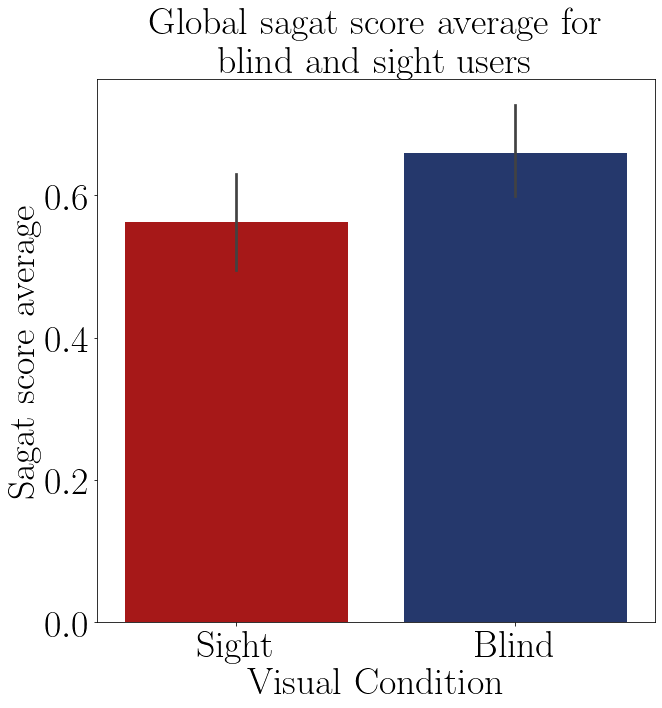
\includegraphics[width = \linewidth]{Resultados/Sagat/Figuras/png/barplot_sagat_avg_global.png}
        %\resizebox{0.6\linewidth}{!}{
        %%% Creator: Matplotlib, PGF backend
%%
%% To include the figure in your LaTeX document, write
%%   \input{<filename>.pgf}
%%
%% Make sure the required packages are loaded in your preamble
%%   \usepackage{pgf}
%%
%% Figures using additional raster images can only be included by \input if
%% they are in the same directory as the main LaTeX file. For loading figures
%% from other directories you can use the `import` package
%%   \usepackage{import}
%%
%% and then include the figures with
%%   \import{<path to file>}{<filename>.pgf}
%%
%% Matplotlib used the following preamble
%%   \usepackage{fontspec}
%%
\begingroup%
\makeatletter%
\begin{pgfpicture}%
\pgfpathrectangle{\pgfpointorigin}{\pgfqpoint{8.990505in}{9.874752in}}%
\pgfusepath{use as bounding box, clip}%
\begin{pgfscope}%
\pgfsetbuttcap%
\pgfsetmiterjoin%
\pgfsetlinewidth{0.000000pt}%
\definecolor{currentstroke}{rgb}{1.000000,1.000000,1.000000}%
\pgfsetstrokecolor{currentstroke}%
\pgfsetstrokeopacity{0.000000}%
\pgfsetdash{}{0pt}%
\pgfpathmoveto{\pgfqpoint{0.000000in}{0.000000in}}%
\pgfpathlineto{\pgfqpoint{8.990505in}{0.000000in}}%
\pgfpathlineto{\pgfqpoint{8.990505in}{9.874752in}}%
\pgfpathlineto{\pgfqpoint{0.000000in}{9.874752in}}%
\pgfpathclose%
\pgfusepath{}%
\end{pgfscope}%
\begin{pgfscope}%
\pgfsetbuttcap%
\pgfsetmiterjoin%
\definecolor{currentfill}{rgb}{1.000000,1.000000,1.000000}%
\pgfsetfillcolor{currentfill}%
\pgfsetlinewidth{0.000000pt}%
\definecolor{currentstroke}{rgb}{0.000000,0.000000,0.000000}%
\pgfsetstrokecolor{currentstroke}%
\pgfsetstrokeopacity{0.000000}%
\pgfsetdash{}{0pt}%
\pgfpathmoveto{\pgfqpoint{1.140505in}{1.198954in}}%
\pgfpathlineto{\pgfqpoint{8.890505in}{1.198954in}}%
\pgfpathlineto{\pgfqpoint{8.890505in}{8.748954in}}%
\pgfpathlineto{\pgfqpoint{1.140505in}{8.748954in}}%
\pgfpathclose%
\pgfusepath{fill}%
\end{pgfscope}%
\begin{pgfscope}%
\pgfpathrectangle{\pgfqpoint{1.140505in}{1.198954in}}{\pgfqpoint{7.750000in}{7.550000in}}%
\pgfusepath{clip}%
\pgfsetbuttcap%
\pgfsetmiterjoin%
\definecolor{currentfill}{rgb}{0.651961,0.093137,0.093137}%
\pgfsetfillcolor{currentfill}%
\pgfsetlinewidth{0.000000pt}%
\definecolor{currentstroke}{rgb}{0.000000,0.000000,0.000000}%
\pgfsetstrokecolor{currentstroke}%
\pgfsetstrokeopacity{0.000000}%
\pgfsetdash{}{0pt}%
\pgfpathmoveto{\pgfqpoint{1.528005in}{1.198954in}}%
\pgfpathlineto{\pgfqpoint{4.628005in}{1.198954in}}%
\pgfpathlineto{\pgfqpoint{4.628005in}{6.762738in}}%
\pgfpathlineto{\pgfqpoint{1.528005in}{6.762738in}}%
\pgfpathclose%
\pgfusepath{fill}%
\end{pgfscope}%
\begin{pgfscope}%
\pgfpathrectangle{\pgfqpoint{1.140505in}{1.198954in}}{\pgfqpoint{7.750000in}{7.550000in}}%
\pgfusepath{clip}%
\pgfsetbuttcap%
\pgfsetmiterjoin%
\definecolor{currentfill}{rgb}{0.144608,0.218137,0.424020}%
\pgfsetfillcolor{currentfill}%
\pgfsetlinewidth{0.000000pt}%
\definecolor{currentstroke}{rgb}{0.000000,0.000000,0.000000}%
\pgfsetstrokecolor{currentstroke}%
\pgfsetstrokeopacity{0.000000}%
\pgfsetdash{}{0pt}%
\pgfpathmoveto{\pgfqpoint{5.403005in}{1.198954in}}%
\pgfpathlineto{\pgfqpoint{8.503005in}{1.198954in}}%
\pgfpathlineto{\pgfqpoint{8.503005in}{7.732572in}}%
\pgfpathlineto{\pgfqpoint{5.403005in}{7.732572in}}%
\pgfpathclose%
\pgfusepath{fill}%
\end{pgfscope}%
\begin{pgfscope}%
\pgfsetbuttcap%
\pgfsetroundjoin%
\definecolor{currentfill}{rgb}{0.000000,0.000000,0.000000}%
\pgfsetfillcolor{currentfill}%
\pgfsetlinewidth{0.803000pt}%
\definecolor{currentstroke}{rgb}{0.000000,0.000000,0.000000}%
\pgfsetstrokecolor{currentstroke}%
\pgfsetdash{}{0pt}%
\pgfsys@defobject{currentmarker}{\pgfqpoint{0.000000in}{-0.048611in}}{\pgfqpoint{0.000000in}{0.000000in}}{%
\pgfpathmoveto{\pgfqpoint{0.000000in}{0.000000in}}%
\pgfpathlineto{\pgfqpoint{0.000000in}{-0.048611in}}%
\pgfusepath{stroke,fill}%
}%
\begin{pgfscope}%
\pgfsys@transformshift{3.078005in}{1.198954in}%
\pgfsys@useobject{currentmarker}{}%
\end{pgfscope}%
\end{pgfscope}%
\begin{pgfscope}%
\definecolor{textcolor}{rgb}{0.000000,0.000000,0.000000}%
\pgfsetstrokecolor{textcolor}%
\pgfsetfillcolor{textcolor}%
\pgftext[x=3.078005in,y=1.101732in,,top]{\color{textcolor}\rmfamily\fontsize{38.016000}{45.619200}\selectfont Sight}%
\end{pgfscope}%
\begin{pgfscope}%
\pgfsetbuttcap%
\pgfsetroundjoin%
\definecolor{currentfill}{rgb}{0.000000,0.000000,0.000000}%
\pgfsetfillcolor{currentfill}%
\pgfsetlinewidth{0.803000pt}%
\definecolor{currentstroke}{rgb}{0.000000,0.000000,0.000000}%
\pgfsetstrokecolor{currentstroke}%
\pgfsetdash{}{0pt}%
\pgfsys@defobject{currentmarker}{\pgfqpoint{0.000000in}{-0.048611in}}{\pgfqpoint{0.000000in}{0.000000in}}{%
\pgfpathmoveto{\pgfqpoint{0.000000in}{0.000000in}}%
\pgfpathlineto{\pgfqpoint{0.000000in}{-0.048611in}}%
\pgfusepath{stroke,fill}%
}%
\begin{pgfscope}%
\pgfsys@transformshift{6.953005in}{1.198954in}%
\pgfsys@useobject{currentmarker}{}%
\end{pgfscope}%
\end{pgfscope}%
\begin{pgfscope}%
\definecolor{textcolor}{rgb}{0.000000,0.000000,0.000000}%
\pgfsetstrokecolor{textcolor}%
\pgfsetfillcolor{textcolor}%
\pgftext[x=6.953005in,y=1.101732in,,top]{\color{textcolor}\rmfamily\fontsize{38.016000}{45.619200}\selectfont Blind}%
\end{pgfscope}%
\begin{pgfscope}%
\definecolor{textcolor}{rgb}{0.000000,0.000000,0.000000}%
\pgfsetstrokecolor{textcolor}%
\pgfsetfillcolor{textcolor}%
\pgftext[x=5.015505in,y=0.569392in,,top]{\color{textcolor}\rmfamily\fontsize{38.016000}{45.619200}\selectfont Visual Condition}%
\end{pgfscope}%
\begin{pgfscope}%
\pgfsetbuttcap%
\pgfsetroundjoin%
\definecolor{currentfill}{rgb}{0.000000,0.000000,0.000000}%
\pgfsetfillcolor{currentfill}%
\pgfsetlinewidth{0.803000pt}%
\definecolor{currentstroke}{rgb}{0.000000,0.000000,0.000000}%
\pgfsetstrokecolor{currentstroke}%
\pgfsetdash{}{0pt}%
\pgfsys@defobject{currentmarker}{\pgfqpoint{-0.048611in}{0.000000in}}{\pgfqpoint{-0.000000in}{0.000000in}}{%
\pgfpathmoveto{\pgfqpoint{-0.000000in}{0.000000in}}%
\pgfpathlineto{\pgfqpoint{-0.048611in}{0.000000in}}%
\pgfusepath{stroke,fill}%
}%
\begin{pgfscope}%
\pgfsys@transformshift{1.140505in}{1.198954in}%
\pgfsys@useobject{currentmarker}{}%
\end{pgfscope}%
\end{pgfscope}%
\begin{pgfscope}%
\definecolor{textcolor}{rgb}{0.000000,0.000000,0.000000}%
\pgfsetstrokecolor{textcolor}%
\pgfsetfillcolor{textcolor}%
\pgftext[x=0.632340in, y=1.015738in, left, base]{\color{textcolor}\rmfamily\fontsize{38.016000}{45.619200}\selectfont \(\displaystyle {0.0}\)}%
\end{pgfscope}%
\begin{pgfscope}%
\pgfsetbuttcap%
\pgfsetroundjoin%
\definecolor{currentfill}{rgb}{0.000000,0.000000,0.000000}%
\pgfsetfillcolor{currentfill}%
\pgfsetlinewidth{0.803000pt}%
\definecolor{currentstroke}{rgb}{0.000000,0.000000,0.000000}%
\pgfsetstrokecolor{currentstroke}%
\pgfsetdash{}{0pt}%
\pgfsys@defobject{currentmarker}{\pgfqpoint{-0.048611in}{0.000000in}}{\pgfqpoint{-0.000000in}{0.000000in}}{%
\pgfpathmoveto{\pgfqpoint{-0.000000in}{0.000000in}}%
\pgfpathlineto{\pgfqpoint{-0.048611in}{0.000000in}}%
\pgfusepath{stroke,fill}%
}%
\begin{pgfscope}%
\pgfsys@transformshift{1.140505in}{3.178838in}%
\pgfsys@useobject{currentmarker}{}%
\end{pgfscope}%
\end{pgfscope}%
\begin{pgfscope}%
\definecolor{textcolor}{rgb}{0.000000,0.000000,0.000000}%
\pgfsetstrokecolor{textcolor}%
\pgfsetfillcolor{textcolor}%
\pgftext[x=0.632340in, y=2.995622in, left, base]{\color{textcolor}\rmfamily\fontsize{38.016000}{45.619200}\selectfont \(\displaystyle {0.2}\)}%
\end{pgfscope}%
\begin{pgfscope}%
\pgfsetbuttcap%
\pgfsetroundjoin%
\definecolor{currentfill}{rgb}{0.000000,0.000000,0.000000}%
\pgfsetfillcolor{currentfill}%
\pgfsetlinewidth{0.803000pt}%
\definecolor{currentstroke}{rgb}{0.000000,0.000000,0.000000}%
\pgfsetstrokecolor{currentstroke}%
\pgfsetdash{}{0pt}%
\pgfsys@defobject{currentmarker}{\pgfqpoint{-0.048611in}{0.000000in}}{\pgfqpoint{-0.000000in}{0.000000in}}{%
\pgfpathmoveto{\pgfqpoint{-0.000000in}{0.000000in}}%
\pgfpathlineto{\pgfqpoint{-0.048611in}{0.000000in}}%
\pgfusepath{stroke,fill}%
}%
\begin{pgfscope}%
\pgfsys@transformshift{1.140505in}{5.158723in}%
\pgfsys@useobject{currentmarker}{}%
\end{pgfscope}%
\end{pgfscope}%
\begin{pgfscope}%
\definecolor{textcolor}{rgb}{0.000000,0.000000,0.000000}%
\pgfsetstrokecolor{textcolor}%
\pgfsetfillcolor{textcolor}%
\pgftext[x=0.632340in, y=4.975506in, left, base]{\color{textcolor}\rmfamily\fontsize{38.016000}{45.619200}\selectfont \(\displaystyle {0.4}\)}%
\end{pgfscope}%
\begin{pgfscope}%
\pgfsetbuttcap%
\pgfsetroundjoin%
\definecolor{currentfill}{rgb}{0.000000,0.000000,0.000000}%
\pgfsetfillcolor{currentfill}%
\pgfsetlinewidth{0.803000pt}%
\definecolor{currentstroke}{rgb}{0.000000,0.000000,0.000000}%
\pgfsetstrokecolor{currentstroke}%
\pgfsetdash{}{0pt}%
\pgfsys@defobject{currentmarker}{\pgfqpoint{-0.048611in}{0.000000in}}{\pgfqpoint{-0.000000in}{0.000000in}}{%
\pgfpathmoveto{\pgfqpoint{-0.000000in}{0.000000in}}%
\pgfpathlineto{\pgfqpoint{-0.048611in}{0.000000in}}%
\pgfusepath{stroke,fill}%
}%
\begin{pgfscope}%
\pgfsys@transformshift{1.140505in}{7.138607in}%
\pgfsys@useobject{currentmarker}{}%
\end{pgfscope}%
\end{pgfscope}%
\begin{pgfscope}%
\definecolor{textcolor}{rgb}{0.000000,0.000000,0.000000}%
\pgfsetstrokecolor{textcolor}%
\pgfsetfillcolor{textcolor}%
\pgftext[x=0.632340in, y=6.955391in, left, base]{\color{textcolor}\rmfamily\fontsize{38.016000}{45.619200}\selectfont \(\displaystyle {0.6}\)}%
\end{pgfscope}%
\begin{pgfscope}%
\definecolor{textcolor}{rgb}{0.000000,0.000000,0.000000}%
\pgfsetstrokecolor{textcolor}%
\pgfsetfillcolor{textcolor}%
\pgftext[x=0.576784in,y=4.973954in,,bottom,rotate=90.000000]{\color{textcolor}\rmfamily\fontsize{38.016000}{45.619200}\selectfont Sagat score average}%
\end{pgfscope}%
\begin{pgfscope}%
\pgfpathrectangle{\pgfqpoint{1.140505in}{1.198954in}}{\pgfqpoint{7.750000in}{7.550000in}}%
\pgfusepath{clip}%
\pgfsetrectcap%
\pgfsetroundjoin%
\pgfsetlinewidth{2.710125pt}%
\definecolor{currentstroke}{rgb}{0.260000,0.260000,0.260000}%
\pgfsetstrokecolor{currentstroke}%
\pgfsetdash{}{0pt}%
\pgfpathmoveto{\pgfqpoint{3.078005in}{6.090776in}}%
\pgfpathlineto{\pgfqpoint{3.078005in}{7.385195in}}%
\pgfusepath{stroke}%
\end{pgfscope}%
\begin{pgfscope}%
\pgfpathrectangle{\pgfqpoint{1.140505in}{1.198954in}}{\pgfqpoint{7.750000in}{7.550000in}}%
\pgfusepath{clip}%
\pgfsetrectcap%
\pgfsetroundjoin%
\pgfsetlinewidth{2.710125pt}%
\definecolor{currentstroke}{rgb}{0.260000,0.260000,0.260000}%
\pgfsetstrokecolor{currentstroke}%
\pgfsetdash{}{0pt}%
\pgfpathmoveto{\pgfqpoint{6.953005in}{7.125552in}}%
\pgfpathlineto{\pgfqpoint{6.953005in}{8.389430in}}%
\pgfusepath{stroke}%
\end{pgfscope}%
\begin{pgfscope}%
\pgfsetrectcap%
\pgfsetmiterjoin%
\pgfsetlinewidth{0.803000pt}%
\definecolor{currentstroke}{rgb}{0.000000,0.000000,0.000000}%
\pgfsetstrokecolor{currentstroke}%
\pgfsetdash{}{0pt}%
\pgfpathmoveto{\pgfqpoint{1.140505in}{1.198954in}}%
\pgfpathlineto{\pgfqpoint{1.140505in}{8.748954in}}%
\pgfusepath{stroke}%
\end{pgfscope}%
\begin{pgfscope}%
\pgfsetrectcap%
\pgfsetmiterjoin%
\pgfsetlinewidth{0.803000pt}%
\definecolor{currentstroke}{rgb}{0.000000,0.000000,0.000000}%
\pgfsetstrokecolor{currentstroke}%
\pgfsetdash{}{0pt}%
\pgfpathmoveto{\pgfqpoint{8.890505in}{1.198954in}}%
\pgfpathlineto{\pgfqpoint{8.890505in}{8.748954in}}%
\pgfusepath{stroke}%
\end{pgfscope}%
\begin{pgfscope}%
\pgfsetrectcap%
\pgfsetmiterjoin%
\pgfsetlinewidth{0.803000pt}%
\definecolor{currentstroke}{rgb}{0.000000,0.000000,0.000000}%
\pgfsetstrokecolor{currentstroke}%
\pgfsetdash{}{0pt}%
\pgfpathmoveto{\pgfqpoint{1.140505in}{1.198954in}}%
\pgfpathlineto{\pgfqpoint{8.890505in}{1.198954in}}%
\pgfusepath{stroke}%
\end{pgfscope}%
\begin{pgfscope}%
\pgfsetrectcap%
\pgfsetmiterjoin%
\pgfsetlinewidth{0.803000pt}%
\definecolor{currentstroke}{rgb}{0.000000,0.000000,0.000000}%
\pgfsetstrokecolor{currentstroke}%
\pgfsetdash{}{0pt}%
\pgfpathmoveto{\pgfqpoint{1.140505in}{8.748954in}}%
\pgfpathlineto{\pgfqpoint{8.890505in}{8.748954in}}%
\pgfusepath{stroke}%
\end{pgfscope}%
\begin{pgfscope}%
\definecolor{textcolor}{rgb}{0.000000,0.000000,0.000000}%
\pgfsetstrokecolor{textcolor}%
\pgfsetfillcolor{textcolor}%
\pgftext[x=1.767248in, y=9.404096in, left, base]{\color{textcolor}\rmfamily\fontsize{38.016000}{45.619200}\selectfont Global sagat score average for }%
\end{pgfscope}%
\begin{pgfscope}%
\definecolor{textcolor}{rgb}{0.000000,0.000000,0.000000}%
\pgfsetstrokecolor{textcolor}%
\pgfsetfillcolor{textcolor}%
\pgftext[x=2.820080in, y=8.856666in, left, base]{\color{textcolor}\rmfamily\fontsize{38.016000}{45.619200}\selectfont   blind and sight users}%
\end{pgfscope}%
\end{pgfpicture}%
\makeatother%
\endgroup%

        %}
        \caption{Barplot of the average Sagat score of each group.}
        \label{fig:barplot_sagat}
    \end{minipage}
\end{figure}


The Shapiro–Wilk normality test on the Table \ref{tab:shapiro_sagat_score} shows that these data are normally distributed, with a p-value higher than 0.05, then it is possible to perform a T-Test to guarantee that the "blind" sample is different then the "sight" sample.

%
\begin{table}[!htb]
\centering
\caption{Shapiro test p-value for the Sagat score for each method and visual condition}
\label{tab:shapiro_sagat_score}
\begin{tabular}{lr}
\toprule
                    Method &  Shapiro P-Value \\
\midrule
        Base blinded users &            0.619 \\
        Base blinded users &            1.000 \\
       Audio blinded users &            0.202 \\
       Audio blinded users &            0.606 \\
 Haptic Belt blinded users &            0.137 \\
 Haptic Belt blinded users &            0.715 \\
Virtual Cane blinded users &            0.326 \\
Virtual Cane blinded users &            0.909 \\
     Mixture blinded users &            0.124 \\
     Mixture blinded users &            0.641 \\
\bottomrule
\end{tabular}
\end{table}



Acording to the T-Test presented on the Table \ref{tab:ttest_sagat_score}, the only method that showed a difference on the Sagat score between the "sight" sample and the "blind" sample is the "Base" method. The other methods both samples had a similar Sagat score.

%
\begin{table}[!htb]
\centering
\caption{T test p-value for the Sagat score on each method for blinded users versus sighted users.}
\label{tab:ttest_sagat_score}
\begin{tabular}{lr}
\toprule
      Method &  T-Test P-Value \\
\midrule
        Base &           0.007 \\
       Audio &           0.561 \\
 Haptic Belt &           0.527 \\
Virtual Cane &           0.230 \\
     Mixture &           0.488 \\
\bottomrule
\end{tabular}
\end{table}



\begin{table}[!htb]
    \begin{minipage}{.45\linewidth}
        
\centering
\caption{Shapiro test p-value for the Sagat score for each method and visual condition}
\label{tab:shapiro_sagat_score}
\begin{tabular}{lr}
\toprule
            Method &  Shapiro P-Value \\
\midrule
        Base blind &            0.189 \\
        Base sight &            1.000 \\
       Audio blind &            0.350 \\
       Audio sight &            0.925 \\
 Haptic Belt blind &            0.315 \\
 Haptic Belt sight &            0.942 \\
Virtual Cane blind &            0.549 \\
Virtual Cane sight &            0.784 \\
     Mixture blind &            0.520 \\
     Mixture sight &            0.446 \\
\bottomrule
\end{tabular}

    \end{minipage}
    \hfill
    \begin{minipage}{.45\linewidth}
        \vspace{-2.75cm}
        
\centering
\caption{T test p-value for the Sagat score on each method for blinded users versus sighted users.}
\label{tab:ttest_sagat_score}
\begin{tabular}{lr}
\toprule
      Method &  T-Test P-Value \\
\midrule
        Base &           0.007 \\
       Audio &           0.561 \\
 Haptic Belt &           0.527 \\
Virtual Cane &           0.230 \\
     Mixture &           0.488 \\
\bottomrule
\end{tabular}

    \end{minipage}
\end{table}

The Table \ref{tab:anova_sagat_avg} shows the Anova test p-value of the Sagat score average of the "blind" sample between the guidance methods presented on the Table \ref{tab:sagat_average}. The p-value indicates that there is at least one method that is statistically equal to one of the other methods.


\begin{table}[!htb]
\centering
\caption{Anova p-value for the Sagat score on each method for blinded users.}
\label{tab:anova_sagat_avg}
\begin{tabular}{lrrrrr}
\toprule
         Source &  Squared sum &  DOF & Squared average &     F & \begin{tabular}[c]{@{}l@{}}P-Value \\ $(F_{0} > F)$\end{tabular} \\
\midrule
Between factors &        0.089 &    4 &           0.022 & 0.684 &                                                            0.608 \\
 Inside factors &        1.142 &   35 &           0.033 &       &                                                                  \\
          Total &        1.231 &   39 &                 &       &                                                                  \\
\bottomrule
\end{tabular}
\end{table}



The Table \ref{tab:lsd_sagat_avg} presents the analysis of a pairwise Fisher LSD test of the blind average Sagat score  between all the guidance methods. The results show that only "Virtual Cane" caused a different average score than the one notice on the "Base" Method. The rest of the methods are did not signifcally chance it.


\begin{table}[!htb]
\centering
\caption{Cross validation p-value for the Sagat score on each method for blinded users.}
\label{tab:lsd_sagat_avg}
\begin{tabular}{rclr}
\toprule
      \multicolumn{3}{c}{Method} &                                       Analysis \\
\midrule
              Base & $X$ & Audio &               $H_0 : \mu_{Base} = \mu_{Audio}$ \\
        Base & $X$ & Haptic Belt &         $H_0 : \mu_{Base} = \mu_{Haptic Belt}$ \\
       Base & $X$ & Virtual Cane &    $H_1 : \mu_{Base} \ne \mu_{Virtual Cane}**$ \\
            Base & $X$ & Mixture &             $H_0 : \mu_{Base} = \mu_{Mixture}$ \\
       Audio & $X$ & Haptic Belt &        $H_0 : \mu_{Audio} = \mu_{Haptic Belt}$ \\
      Audio & $X$ & Virtual Cane &       $H_0 : \mu_{Audio} = \mu_{Virtual Cane}$ \\
           Audio & $X$ & Mixture &            $H_0 : \mu_{Audio} = \mu_{Mixture}$ \\
Haptic Belt & $X$ & Virtual Cane & $H_0 : \mu_{Haptic Belt} = \mu_{Virtual Cane}$ \\
     Haptic Belt & $X$ & Mixture &      $H_0 : \mu_{Haptic Belt} = \mu_{Mixture}$ \\
    Virtual Cane & $X$ & Mixture & $H_1 : \mu_{Virtual Cane} \ne \mu_{Mixture}**$ \\
\bottomrule
\end{tabular}
\end{table}



The Table \ref{tab:anova_sagat_var} shows the Anova test p-value of the Sagat score variation of the "blind" sample between the guidance methods presented on the Table \ref{tab:sagat_var}. The p-value indicates that there is at least one method that is statistically equal to one of the other methods so its recommended to do a pairwise analyses between all the methods.


\begin{table}[!htb]
\centering
\caption{Adapted SAGAT global score variation grouped by participant and guidance method.}
\label{tab:sagat_var}
\begin{tabular}{lrrrrrr}
\toprule
{} &     Base &    Audio & \begin{tabular}[c]{@{}l@{}}Haptic\\ Belt\end{tabular} & \begin{tabular}[c]{@{}l@{}}Virtual\\ Cane\end{tabular} &  Mixture & \begin{tabular}[c]{@{}l@{}}Visual\\ Condition\end{tabular} \\
Participant &          &          &                                                       &                                                        &          &                                                            \\
\midrule
001         &    0.0\% &   33.3\% &                                                15.5\% &                                                 88.0\% &  -30.8\% &                                                      Sight \\
001C        &    0.0\% &   18.2\% &                                                59.5\% &                                                 -5.7\% &   57.1\% &                                                      Blind \\
002C        &  -22.2\% &   11.1\% &                                                 0.3\% &                                                 44.4\% &   36.0\% &                                                      Blind \\
003         &    0.0\% &  -11.1\% &                                                21.0\% &                                                 56.6\% &   11.1\% &                                                      Sight \\
003C        &   37.9\% &   33.3\% &                                                13.5\% &                                                 93.1\% &    0.0\% &                                                      Blind \\
004         &    0.0\% &    6.9\% &                                                18.9\% &                                                 37.7\% &  -15.2\% &                                                      Sight \\
004C        &   20.0\% &    0.0\% &                                                20.8\% &                                                 45.3\% &   38.5\% &                                                      Blind \\
005         &    0.0\% &   25.0\% &                                                -5.1\% &                                                -49.9\% &   50.0\% &                                                      Sight \\
\bottomrule
\end{tabular}
\end{table}




\begin{table}[!htb]
\centering
\caption{Anova p-value for the variation Sagat score on each method for blinded users.}
\label{tab:anova_sagat_var}
\begin{tabular}{lrrrrr}
\toprule
         Source &  Squared sum &  DOF & Squared average &     F & p-Value (F\_0 > F) \\
\midrule
Between factors &     3131.542 &    4 &         782.885 & 1.055 &             0.412 \\
 Inside factors &    11133.360 &   15 &         742.224 &       &                   \\
          Total &    14264.902 &   19 &                 &       &                   \\
\bottomrule
\end{tabular}
\end{table}



The Table \ref{tab:lsd_sagat_var} presents the conclusion of a pairwise Fisher LSD test of the blind Sagat score variation between all the guidance methods. The results show that the ""Haptic Belt" and the "Mixture" method have a different variation then the "Base" method and they are also different between each other. This can be seen at the Table \ref{tab:sagat_var_average_group} and in the Figure \ref{fig:barplot_sagat_var_scene_blind} compiles the Sagat score average of the methods observed on all of the participants.


\begin{table}[!htb]
\centering
\caption{Cross validation p-value for the variation Sagat score on each method for blinded users.}
\label{tab:lsd_sagat_var}
\begin{tabular}{lr}
\toprule
                         Method &                                           Analysis \\
\midrule
              Base versus Audio &                   $H_0 : \mu_{Base} = \mu_{Audio}$ \\
        Base versus Haptic Belt &             $H_0 : \mu_{Base} = \mu_{Haptic Belt}$ \\
       Base versus Virtual Cane &        $H_1 : \mu_{Base} \ne \mu_{Virtual Cane}**$ \\
            Base versus Mixture &             $H_1 : \mu_{Base} \ne \mu_{Mixture}**$ \\
       Audio versus Haptic Belt &            $H_0 : \mu_{Audio} = \mu_{Haptic Belt}$ \\
      Audio versus Virtual Cane &       $H_1 : \mu_{Audio} \ne \mu_{Virtual Cane}**$ \\
           Audio versus Mixture &            $H_1 : \mu_{Audio} \ne \mu_{Mixture}**$ \\
Haptic Belt versus Virtual Cane & $H_1 : \mu_{Haptic Belt} \ne \mu_{Virtual Cane}**$ \\
     Haptic Belt versus Mixture &          $H_0 : \mu_{Haptic Belt} = \mu_{Mixture}$ \\
    Virtual Cane versus Mixture &         $H_0 : \mu_{Virtual Cane} = \mu_{Mixture}$ \\
\bottomrule
\end{tabular}
\end{table}




\begin{table}[!htb]
\centering
\caption{Adapted Sagat global score variation grouped by participant and visual Condition}
\label{tab:sagat_var_average_group}
\begin{tabular}{lrrrrrr}
\toprule
{} &  Base &  Audio & \begin{tabular}[c]{@{}l@{}}Haptic\\ Belt\end{tabular} & \begin{tabular}[c]{@{}l@{}}Virtual\\ Cane\end{tabular} &  Mixture \\
Visual Condition &       &        &                                                       &                                                        &          \\
\midrule
Blind            &  8.93 &  15.66 &                                                 23.49 &                                                  44.30 &   32.901 \\
Sight            &  0.00 &  13.53 &                                                 12.59 &                                                  33.12 &    3.798 \\
\bottomrule
\end{tabular}
\end{table}



\begin{figure}[!htb]
    \centering
    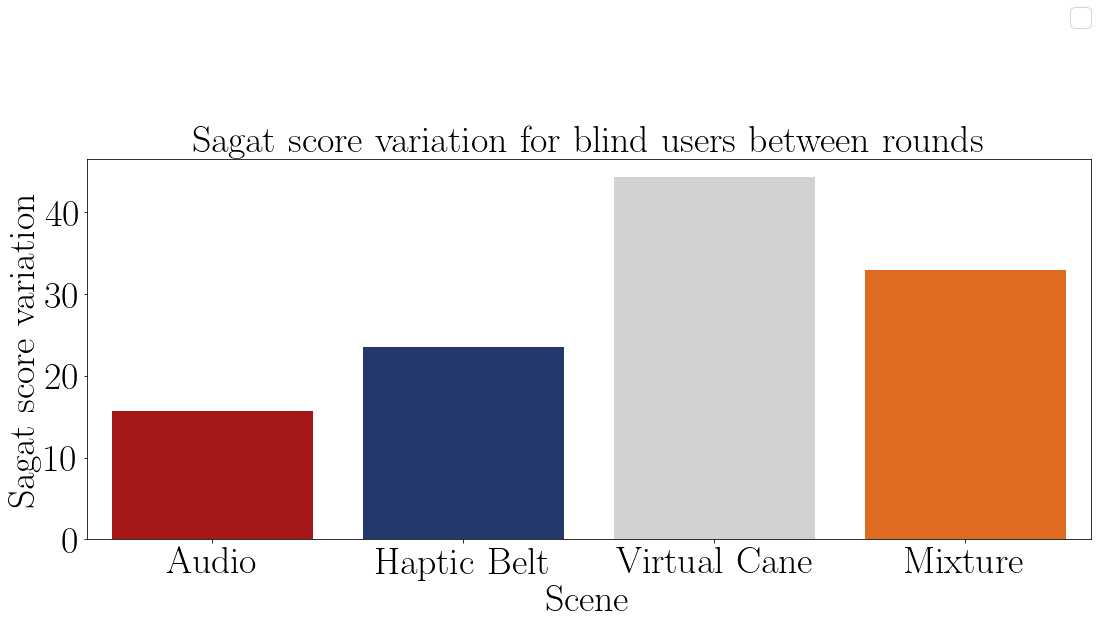
\includegraphics[width = 0.8\linewidth]{Resultados/Sagat/Figuras/png/barplot_sagat_var_scene_blind.png}
    %\resizebox{0.6\linewidth}{!}{
    %%% Creator: Matplotlib, PGF backend
%%
%% To include the figure in your LaTeX document, write
%%   \input{<filename>.pgf}
%%
%% Make sure the required packages are loaded in your preamble
%%   \usepackage{pgf}
%%
%% and, on pdftex
%%   \usepackage[utf8]{inputenc}\DeclareUnicodeCharacter{2212}{-}
%%
%% or, on luatex and xetex
%%   \usepackage{unicode-math}
%%
%% Figures using additional raster images can only be included by \input if
%% they are in the same directory as the main LaTeX file. For loading figures
%% from other directories you can use the `import` package
%%   \usepackage{import}
%%
%% and then include the figures with
%%   \import{<path to file>}{<filename>.pgf}
%%
%% Matplotlib used the following preamble
%%   \usepackage{url}
%%   \usepackage{unicode-math}
%%   \setmainfont{DejaVu Serif}
%%   \usepackage{fontspec}
%%
\begingroup%
\makeatletter%
\begin{pgfpicture}%
\pgfpathrectangle{\pgfpointorigin}{\pgfqpoint{14.459096in}{14.522618in}}%
\pgfusepath{use as bounding box, clip}%
\begin{pgfscope}%
\pgfsetbuttcap%
\pgfsetmiterjoin%
\pgfsetlinewidth{0.000000pt}%
\definecolor{currentstroke}{rgb}{1.000000,1.000000,1.000000}%
\pgfsetstrokecolor{currentstroke}%
\pgfsetstrokeopacity{0.000000}%
\pgfsetdash{}{0pt}%
\pgfpathmoveto{\pgfqpoint{0.000000in}{0.000000in}}%
\pgfpathlineto{\pgfqpoint{14.459096in}{0.000000in}}%
\pgfpathlineto{\pgfqpoint{14.459096in}{14.522618in}}%
\pgfpathlineto{\pgfqpoint{0.000000in}{14.522618in}}%
\pgfpathclose%
\pgfusepath{}%
\end{pgfscope}%
\begin{pgfscope}%
\pgfsetbuttcap%
\pgfsetmiterjoin%
\definecolor{currentfill}{rgb}{1.000000,1.000000,1.000000}%
\pgfsetfillcolor{currentfill}%
\pgfsetlinewidth{0.000000pt}%
\definecolor{currentstroke}{rgb}{0.000000,0.000000,0.000000}%
\pgfsetstrokecolor{currentstroke}%
\pgfsetstrokeopacity{0.000000}%
\pgfsetdash{}{0pt}%
\pgfpathmoveto{\pgfqpoint{1.804548in}{1.104418in}}%
\pgfpathlineto{\pgfqpoint{12.654548in}{1.104418in}}%
\pgfpathlineto{\pgfqpoint{12.654548in}{11.674418in}}%
\pgfpathlineto{\pgfqpoint{1.804548in}{11.674418in}}%
\pgfpathclose%
\pgfusepath{fill}%
\end{pgfscope}%
\begin{pgfscope}%
\pgfpathrectangle{\pgfqpoint{1.804548in}{1.104418in}}{\pgfqpoint{10.850000in}{10.570000in}}%
\pgfusepath{clip}%
\pgfsetbuttcap%
\pgfsetmiterjoin%
\definecolor{currentfill}{rgb}{0.651961,0.093137,0.093137}%
\pgfsetfillcolor{currentfill}%
\pgfsetlinewidth{0.000000pt}%
\definecolor{currentstroke}{rgb}{0.000000,0.000000,0.000000}%
\pgfsetstrokecolor{currentstroke}%
\pgfsetstrokeopacity{0.000000}%
\pgfsetdash{}{0pt}%
\pgfpathmoveto{\pgfqpoint{2.075798in}{1.104418in}}%
\pgfpathlineto{\pgfqpoint{4.245798in}{1.104418in}}%
\pgfpathlineto{\pgfqpoint{4.245798in}{4.662038in}}%
\pgfpathlineto{\pgfqpoint{2.075798in}{4.662038in}}%
\pgfpathclose%
\pgfusepath{fill}%
\end{pgfscope}%
\begin{pgfscope}%
\pgfpathrectangle{\pgfqpoint{1.804548in}{1.104418in}}{\pgfqpoint{10.850000in}{10.570000in}}%
\pgfusepath{clip}%
\pgfsetbuttcap%
\pgfsetmiterjoin%
\definecolor{currentfill}{rgb}{0.144608,0.218137,0.424020}%
\pgfsetfillcolor{currentfill}%
\pgfsetlinewidth{0.000000pt}%
\definecolor{currentstroke}{rgb}{0.000000,0.000000,0.000000}%
\pgfsetstrokecolor{currentstroke}%
\pgfsetstrokeopacity{0.000000}%
\pgfsetdash{}{0pt}%
\pgfpathmoveto{\pgfqpoint{4.788298in}{1.104418in}}%
\pgfpathlineto{\pgfqpoint{6.958298in}{1.104418in}}%
\pgfpathlineto{\pgfqpoint{6.958298in}{6.442424in}}%
\pgfpathlineto{\pgfqpoint{4.788298in}{6.442424in}}%
\pgfpathclose%
\pgfusepath{fill}%
\end{pgfscope}%
\begin{pgfscope}%
\pgfpathrectangle{\pgfqpoint{1.804548in}{1.104418in}}{\pgfqpoint{10.850000in}{10.570000in}}%
\pgfusepath{clip}%
\pgfsetbuttcap%
\pgfsetmiterjoin%
\definecolor{currentfill}{rgb}{0.823529,0.823529,0.823529}%
\pgfsetfillcolor{currentfill}%
\pgfsetlinewidth{0.000000pt}%
\definecolor{currentstroke}{rgb}{0.000000,0.000000,0.000000}%
\pgfsetstrokecolor{currentstroke}%
\pgfsetstrokeopacity{0.000000}%
\pgfsetdash{}{0pt}%
\pgfpathmoveto{\pgfqpoint{7.500798in}{1.104418in}}%
\pgfpathlineto{\pgfqpoint{9.670798in}{1.104418in}}%
\pgfpathlineto{\pgfqpoint{9.670798in}{11.171085in}}%
\pgfpathlineto{\pgfqpoint{7.500798in}{11.171085in}}%
\pgfpathclose%
\pgfusepath{fill}%
\end{pgfscope}%
\begin{pgfscope}%
\pgfpathrectangle{\pgfqpoint{1.804548in}{1.104418in}}{\pgfqpoint{10.850000in}{10.570000in}}%
\pgfusepath{clip}%
\pgfsetbuttcap%
\pgfsetmiterjoin%
\definecolor{currentfill}{rgb}{0.875000,0.419118,0.125000}%
\pgfsetfillcolor{currentfill}%
\pgfsetlinewidth{0.000000pt}%
\definecolor{currentstroke}{rgb}{0.000000,0.000000,0.000000}%
\pgfsetstrokecolor{currentstroke}%
\pgfsetstrokeopacity{0.000000}%
\pgfsetdash{}{0pt}%
\pgfpathmoveto{\pgfqpoint{10.213298in}{1.104418in}}%
\pgfpathlineto{\pgfqpoint{12.383298in}{1.104418in}}%
\pgfpathlineto{\pgfqpoint{12.383298in}{8.580491in}}%
\pgfpathlineto{\pgfqpoint{10.213298in}{8.580491in}}%
\pgfpathclose%
\pgfusepath{fill}%
\end{pgfscope}%
\begin{pgfscope}%
\pgfsetbuttcap%
\pgfsetroundjoin%
\definecolor{currentfill}{rgb}{0.000000,0.000000,0.000000}%
\pgfsetfillcolor{currentfill}%
\pgfsetlinewidth{0.803000pt}%
\definecolor{currentstroke}{rgb}{0.000000,0.000000,0.000000}%
\pgfsetstrokecolor{currentstroke}%
\pgfsetdash{}{0pt}%
\pgfsys@defobject{currentmarker}{\pgfqpoint{0.000000in}{-0.048611in}}{\pgfqpoint{0.000000in}{0.000000in}}{%
\pgfpathmoveto{\pgfqpoint{0.000000in}{0.000000in}}%
\pgfpathlineto{\pgfqpoint{0.000000in}{-0.048611in}}%
\pgfusepath{stroke,fill}%
}%
\begin{pgfscope}%
\pgfsys@transformshift{3.160798in}{1.104418in}%
\pgfsys@useobject{currentmarker}{}%
\end{pgfscope}%
\end{pgfscope}%
\begin{pgfscope}%
\definecolor{textcolor}{rgb}{0.000000,0.000000,0.000000}%
\pgfsetstrokecolor{textcolor}%
\pgfsetfillcolor{textcolor}%
\pgftext[x=3.160798in,y=1.007196in,,top]{\color{textcolor}\rmfamily\fontsize{31.680000}{38.016000}\selectfont Audio}%
\end{pgfscope}%
\begin{pgfscope}%
\pgfsetbuttcap%
\pgfsetroundjoin%
\definecolor{currentfill}{rgb}{0.000000,0.000000,0.000000}%
\pgfsetfillcolor{currentfill}%
\pgfsetlinewidth{0.803000pt}%
\definecolor{currentstroke}{rgb}{0.000000,0.000000,0.000000}%
\pgfsetstrokecolor{currentstroke}%
\pgfsetdash{}{0pt}%
\pgfsys@defobject{currentmarker}{\pgfqpoint{0.000000in}{-0.048611in}}{\pgfqpoint{0.000000in}{0.000000in}}{%
\pgfpathmoveto{\pgfqpoint{0.000000in}{0.000000in}}%
\pgfpathlineto{\pgfqpoint{0.000000in}{-0.048611in}}%
\pgfusepath{stroke,fill}%
}%
\begin{pgfscope}%
\pgfsys@transformshift{5.873298in}{1.104418in}%
\pgfsys@useobject{currentmarker}{}%
\end{pgfscope}%
\end{pgfscope}%
\begin{pgfscope}%
\definecolor{textcolor}{rgb}{0.000000,0.000000,0.000000}%
\pgfsetstrokecolor{textcolor}%
\pgfsetfillcolor{textcolor}%
\pgftext[x=5.873298in,y=1.007196in,,top]{\color{textcolor}\rmfamily\fontsize{31.680000}{38.016000}\selectfont Haptic Belt}%
\end{pgfscope}%
\begin{pgfscope}%
\pgfsetbuttcap%
\pgfsetroundjoin%
\definecolor{currentfill}{rgb}{0.000000,0.000000,0.000000}%
\pgfsetfillcolor{currentfill}%
\pgfsetlinewidth{0.803000pt}%
\definecolor{currentstroke}{rgb}{0.000000,0.000000,0.000000}%
\pgfsetstrokecolor{currentstroke}%
\pgfsetdash{}{0pt}%
\pgfsys@defobject{currentmarker}{\pgfqpoint{0.000000in}{-0.048611in}}{\pgfqpoint{0.000000in}{0.000000in}}{%
\pgfpathmoveto{\pgfqpoint{0.000000in}{0.000000in}}%
\pgfpathlineto{\pgfqpoint{0.000000in}{-0.048611in}}%
\pgfusepath{stroke,fill}%
}%
\begin{pgfscope}%
\pgfsys@transformshift{8.585798in}{1.104418in}%
\pgfsys@useobject{currentmarker}{}%
\end{pgfscope}%
\end{pgfscope}%
\begin{pgfscope}%
\definecolor{textcolor}{rgb}{0.000000,0.000000,0.000000}%
\pgfsetstrokecolor{textcolor}%
\pgfsetfillcolor{textcolor}%
\pgftext[x=8.585798in,y=1.007196in,,top]{\color{textcolor}\rmfamily\fontsize{31.680000}{38.016000}\selectfont Virtual Cane}%
\end{pgfscope}%
\begin{pgfscope}%
\pgfsetbuttcap%
\pgfsetroundjoin%
\definecolor{currentfill}{rgb}{0.000000,0.000000,0.000000}%
\pgfsetfillcolor{currentfill}%
\pgfsetlinewidth{0.803000pt}%
\definecolor{currentstroke}{rgb}{0.000000,0.000000,0.000000}%
\pgfsetstrokecolor{currentstroke}%
\pgfsetdash{}{0pt}%
\pgfsys@defobject{currentmarker}{\pgfqpoint{0.000000in}{-0.048611in}}{\pgfqpoint{0.000000in}{0.000000in}}{%
\pgfpathmoveto{\pgfqpoint{0.000000in}{0.000000in}}%
\pgfpathlineto{\pgfqpoint{0.000000in}{-0.048611in}}%
\pgfusepath{stroke,fill}%
}%
\begin{pgfscope}%
\pgfsys@transformshift{11.298298in}{1.104418in}%
\pgfsys@useobject{currentmarker}{}%
\end{pgfscope}%
\end{pgfscope}%
\begin{pgfscope}%
\definecolor{textcolor}{rgb}{0.000000,0.000000,0.000000}%
\pgfsetstrokecolor{textcolor}%
\pgfsetfillcolor{textcolor}%
\pgftext[x=11.298298in,y=1.007196in,,top]{\color{textcolor}\rmfamily\fontsize{31.680000}{38.016000}\selectfont Mixture}%
\end{pgfscope}%
\begin{pgfscope}%
\definecolor{textcolor}{rgb}{0.000000,0.000000,0.000000}%
\pgfsetstrokecolor{textcolor}%
\pgfsetfillcolor{textcolor}%
\pgftext[x=7.229548in,y=0.525820in,,top]{\color{textcolor}\rmfamily\fontsize{31.680000}{38.016000}\selectfont Scene}%
\end{pgfscope}%
\begin{pgfscope}%
\pgfsetbuttcap%
\pgfsetroundjoin%
\definecolor{currentfill}{rgb}{0.000000,0.000000,0.000000}%
\pgfsetfillcolor{currentfill}%
\pgfsetlinewidth{0.803000pt}%
\definecolor{currentstroke}{rgb}{0.000000,0.000000,0.000000}%
\pgfsetstrokecolor{currentstroke}%
\pgfsetdash{}{0pt}%
\pgfsys@defobject{currentmarker}{\pgfqpoint{-0.048611in}{0.000000in}}{\pgfqpoint{-0.000000in}{0.000000in}}{%
\pgfpathmoveto{\pgfqpoint{-0.000000in}{0.000000in}}%
\pgfpathlineto{\pgfqpoint{-0.048611in}{0.000000in}}%
\pgfusepath{stroke,fill}%
}%
\begin{pgfscope}%
\pgfsys@transformshift{1.804548in}{1.104418in}%
\pgfsys@useobject{currentmarker}{}%
\end{pgfscope}%
\end{pgfscope}%
\begin{pgfscope}%
\definecolor{textcolor}{rgb}{0.000000,0.000000,0.000000}%
\pgfsetstrokecolor{textcolor}%
\pgfsetfillcolor{textcolor}%
\pgftext[x=1.487326in, y=0.937270in, left, base]{\color{textcolor}\rmfamily\fontsize{31.680000}{38.016000}\selectfont \(\displaystyle {0}\)}%
\end{pgfscope}%
\begin{pgfscope}%
\pgfsetbuttcap%
\pgfsetroundjoin%
\definecolor{currentfill}{rgb}{0.000000,0.000000,0.000000}%
\pgfsetfillcolor{currentfill}%
\pgfsetlinewidth{0.803000pt}%
\definecolor{currentstroke}{rgb}{0.000000,0.000000,0.000000}%
\pgfsetstrokecolor{currentstroke}%
\pgfsetdash{}{0pt}%
\pgfsys@defobject{currentmarker}{\pgfqpoint{-0.048611in}{0.000000in}}{\pgfqpoint{-0.000000in}{0.000000in}}{%
\pgfpathmoveto{\pgfqpoint{-0.000000in}{0.000000in}}%
\pgfpathlineto{\pgfqpoint{-0.048611in}{0.000000in}}%
\pgfusepath{stroke,fill}%
}%
\begin{pgfscope}%
\pgfsys@transformshift{1.804548in}{3.376705in}%
\pgfsys@useobject{currentmarker}{}%
\end{pgfscope}%
\end{pgfscope}%
\begin{pgfscope}%
\definecolor{textcolor}{rgb}{0.000000,0.000000,0.000000}%
\pgfsetstrokecolor{textcolor}%
\pgfsetfillcolor{textcolor}%
\pgftext[x=1.267326in, y=3.209556in, left, base]{\color{textcolor}\rmfamily\fontsize{31.680000}{38.016000}\selectfont \(\displaystyle {10}\)}%
\end{pgfscope}%
\begin{pgfscope}%
\pgfsetbuttcap%
\pgfsetroundjoin%
\definecolor{currentfill}{rgb}{0.000000,0.000000,0.000000}%
\pgfsetfillcolor{currentfill}%
\pgfsetlinewidth{0.803000pt}%
\definecolor{currentstroke}{rgb}{0.000000,0.000000,0.000000}%
\pgfsetstrokecolor{currentstroke}%
\pgfsetdash{}{0pt}%
\pgfsys@defobject{currentmarker}{\pgfqpoint{-0.048611in}{0.000000in}}{\pgfqpoint{-0.000000in}{0.000000in}}{%
\pgfpathmoveto{\pgfqpoint{-0.000000in}{0.000000in}}%
\pgfpathlineto{\pgfqpoint{-0.048611in}{0.000000in}}%
\pgfusepath{stroke,fill}%
}%
\begin{pgfscope}%
\pgfsys@transformshift{1.804548in}{5.648991in}%
\pgfsys@useobject{currentmarker}{}%
\end{pgfscope}%
\end{pgfscope}%
\begin{pgfscope}%
\definecolor{textcolor}{rgb}{0.000000,0.000000,0.000000}%
\pgfsetstrokecolor{textcolor}%
\pgfsetfillcolor{textcolor}%
\pgftext[x=1.267326in, y=5.481843in, left, base]{\color{textcolor}\rmfamily\fontsize{31.680000}{38.016000}\selectfont \(\displaystyle {20}\)}%
\end{pgfscope}%
\begin{pgfscope}%
\pgfsetbuttcap%
\pgfsetroundjoin%
\definecolor{currentfill}{rgb}{0.000000,0.000000,0.000000}%
\pgfsetfillcolor{currentfill}%
\pgfsetlinewidth{0.803000pt}%
\definecolor{currentstroke}{rgb}{0.000000,0.000000,0.000000}%
\pgfsetstrokecolor{currentstroke}%
\pgfsetdash{}{0pt}%
\pgfsys@defobject{currentmarker}{\pgfqpoint{-0.048611in}{0.000000in}}{\pgfqpoint{-0.000000in}{0.000000in}}{%
\pgfpathmoveto{\pgfqpoint{-0.000000in}{0.000000in}}%
\pgfpathlineto{\pgfqpoint{-0.048611in}{0.000000in}}%
\pgfusepath{stroke,fill}%
}%
\begin{pgfscope}%
\pgfsys@transformshift{1.804548in}{7.921278in}%
\pgfsys@useobject{currentmarker}{}%
\end{pgfscope}%
\end{pgfscope}%
\begin{pgfscope}%
\definecolor{textcolor}{rgb}{0.000000,0.000000,0.000000}%
\pgfsetstrokecolor{textcolor}%
\pgfsetfillcolor{textcolor}%
\pgftext[x=1.267326in, y=7.754129in, left, base]{\color{textcolor}\rmfamily\fontsize{31.680000}{38.016000}\selectfont \(\displaystyle {30}\)}%
\end{pgfscope}%
\begin{pgfscope}%
\pgfsetbuttcap%
\pgfsetroundjoin%
\definecolor{currentfill}{rgb}{0.000000,0.000000,0.000000}%
\pgfsetfillcolor{currentfill}%
\pgfsetlinewidth{0.803000pt}%
\definecolor{currentstroke}{rgb}{0.000000,0.000000,0.000000}%
\pgfsetstrokecolor{currentstroke}%
\pgfsetdash{}{0pt}%
\pgfsys@defobject{currentmarker}{\pgfqpoint{-0.048611in}{0.000000in}}{\pgfqpoint{-0.000000in}{0.000000in}}{%
\pgfpathmoveto{\pgfqpoint{-0.000000in}{0.000000in}}%
\pgfpathlineto{\pgfqpoint{-0.048611in}{0.000000in}}%
\pgfusepath{stroke,fill}%
}%
\begin{pgfscope}%
\pgfsys@transformshift{1.804548in}{10.193564in}%
\pgfsys@useobject{currentmarker}{}%
\end{pgfscope}%
\end{pgfscope}%
\begin{pgfscope}%
\definecolor{textcolor}{rgb}{0.000000,0.000000,0.000000}%
\pgfsetstrokecolor{textcolor}%
\pgfsetfillcolor{textcolor}%
\pgftext[x=1.267326in, y=10.026416in, left, base]{\color{textcolor}\rmfamily\fontsize{31.680000}{38.016000}\selectfont \(\displaystyle {40}\)}%
\end{pgfscope}%
\begin{pgfscope}%
\definecolor{textcolor}{rgb}{0.000000,0.000000,0.000000}%
\pgfsetstrokecolor{textcolor}%
\pgfsetfillcolor{textcolor}%
\pgftext[x=1.211770in,y=6.389418in,,bottom,rotate=90.000000]{\color{textcolor}\rmfamily\fontsize{31.680000}{38.016000}\selectfont Sagat score variation}%
\end{pgfscope}%
\begin{pgfscope}%
\pgfpathrectangle{\pgfqpoint{1.804548in}{1.104418in}}{\pgfqpoint{10.850000in}{10.570000in}}%
\pgfusepath{clip}%
\pgfsetrectcap%
\pgfsetroundjoin%
\pgfsetlinewidth{2.710125pt}%
\definecolor{currentstroke}{rgb}{0.260000,0.260000,0.260000}%
\pgfsetstrokecolor{currentstroke}%
\pgfsetdash{}{0pt}%
\pgfusepath{stroke}%
\end{pgfscope}%
\begin{pgfscope}%
\pgfpathrectangle{\pgfqpoint{1.804548in}{1.104418in}}{\pgfqpoint{10.850000in}{10.570000in}}%
\pgfusepath{clip}%
\pgfsetrectcap%
\pgfsetroundjoin%
\pgfsetlinewidth{2.710125pt}%
\definecolor{currentstroke}{rgb}{0.260000,0.260000,0.260000}%
\pgfsetstrokecolor{currentstroke}%
\pgfsetdash{}{0pt}%
\pgfusepath{stroke}%
\end{pgfscope}%
\begin{pgfscope}%
\pgfpathrectangle{\pgfqpoint{1.804548in}{1.104418in}}{\pgfqpoint{10.850000in}{10.570000in}}%
\pgfusepath{clip}%
\pgfsetrectcap%
\pgfsetroundjoin%
\pgfsetlinewidth{2.710125pt}%
\definecolor{currentstroke}{rgb}{0.260000,0.260000,0.260000}%
\pgfsetstrokecolor{currentstroke}%
\pgfsetdash{}{0pt}%
\pgfusepath{stroke}%
\end{pgfscope}%
\begin{pgfscope}%
\pgfpathrectangle{\pgfqpoint{1.804548in}{1.104418in}}{\pgfqpoint{10.850000in}{10.570000in}}%
\pgfusepath{clip}%
\pgfsetrectcap%
\pgfsetroundjoin%
\pgfsetlinewidth{2.710125pt}%
\definecolor{currentstroke}{rgb}{0.260000,0.260000,0.260000}%
\pgfsetstrokecolor{currentstroke}%
\pgfsetdash{}{0pt}%
\pgfusepath{stroke}%
\end{pgfscope}%
\begin{pgfscope}%
\pgfsetrectcap%
\pgfsetmiterjoin%
\pgfsetlinewidth{0.803000pt}%
\definecolor{currentstroke}{rgb}{0.000000,0.000000,0.000000}%
\pgfsetstrokecolor{currentstroke}%
\pgfsetdash{}{0pt}%
\pgfpathmoveto{\pgfqpoint{1.804548in}{1.104418in}}%
\pgfpathlineto{\pgfqpoint{1.804548in}{11.674418in}}%
\pgfusepath{stroke}%
\end{pgfscope}%
\begin{pgfscope}%
\pgfsetrectcap%
\pgfsetmiterjoin%
\pgfsetlinewidth{0.803000pt}%
\definecolor{currentstroke}{rgb}{0.000000,0.000000,0.000000}%
\pgfsetstrokecolor{currentstroke}%
\pgfsetdash{}{0pt}%
\pgfpathmoveto{\pgfqpoint{12.654548in}{1.104418in}}%
\pgfpathlineto{\pgfqpoint{12.654548in}{11.674418in}}%
\pgfusepath{stroke}%
\end{pgfscope}%
\begin{pgfscope}%
\pgfsetrectcap%
\pgfsetmiterjoin%
\pgfsetlinewidth{0.803000pt}%
\definecolor{currentstroke}{rgb}{0.000000,0.000000,0.000000}%
\pgfsetstrokecolor{currentstroke}%
\pgfsetdash{}{0pt}%
\pgfpathmoveto{\pgfqpoint{1.804548in}{1.104418in}}%
\pgfpathlineto{\pgfqpoint{12.654548in}{1.104418in}}%
\pgfusepath{stroke}%
\end{pgfscope}%
\begin{pgfscope}%
\pgfsetrectcap%
\pgfsetmiterjoin%
\pgfsetlinewidth{0.803000pt}%
\definecolor{currentstroke}{rgb}{0.000000,0.000000,0.000000}%
\pgfsetstrokecolor{currentstroke}%
\pgfsetdash{}{0pt}%
\pgfpathmoveto{\pgfqpoint{1.804548in}{11.674418in}}%
\pgfpathlineto{\pgfqpoint{12.654548in}{11.674418in}}%
\pgfusepath{stroke}%
\end{pgfscope}%
\begin{pgfscope}%
\definecolor{textcolor}{rgb}{0.000000,0.000000,0.000000}%
\pgfsetstrokecolor{textcolor}%
\pgfsetfillcolor{textcolor}%
\pgftext[x=7.229548in,y=11.791723in,,base]{\color{textcolor}\rmfamily\fontsize{38.016000}{45.619200}\selectfont Sagat score variation for blind users between rounds}%
\end{pgfscope}%
\begin{pgfscope}%
\pgfsetbuttcap%
\pgfsetmiterjoin%
\definecolor{currentfill}{rgb}{1.000000,1.000000,1.000000}%
\pgfsetfillcolor{currentfill}%
\pgfsetfillopacity{0.800000}%
\pgfsetlinewidth{1.003750pt}%
\definecolor{currentstroke}{rgb}{0.800000,0.800000,0.800000}%
\pgfsetstrokecolor{currentstroke}%
\pgfsetstrokeopacity{0.800000}%
\pgfsetdash{}{0pt}%
\pgfpathmoveto{\pgfqpoint{12.471215in}{14.178174in}}%
\pgfpathlineto{\pgfqpoint{12.593437in}{14.178174in}}%
\pgfpathquadraticcurveto{\pgfqpoint{12.654548in}{14.178174in}}{\pgfqpoint{12.654548in}{14.239285in}}%
\pgfpathlineto{\pgfqpoint{12.654548in}{14.361507in}}%
\pgfpathquadraticcurveto{\pgfqpoint{12.654548in}{14.422618in}}{\pgfqpoint{12.593437in}{14.422618in}}%
\pgfpathlineto{\pgfqpoint{12.471215in}{14.422618in}}%
\pgfpathquadraticcurveto{\pgfqpoint{12.410103in}{14.422618in}}{\pgfqpoint{12.410103in}{14.361507in}}%
\pgfpathlineto{\pgfqpoint{12.410103in}{14.239285in}}%
\pgfpathquadraticcurveto{\pgfqpoint{12.410103in}{14.178174in}}{\pgfqpoint{12.471215in}{14.178174in}}%
\pgfpathclose%
\pgfusepath{stroke,fill}%
\end{pgfscope}%
\end{pgfpicture}%
\makeatother%
\endgroup%

    %}
    \caption{Barplot of the average Sagat score variation from the blind participants of each method.}
    \label{fig:barplot_sagat_var_scene_blind}
\end{figure}

According to T-Test on Table \ref{tab:ttest_sagat_score}, there is no differecen in Sagat score between the "sight" and the "blind" sample.

According to both Anova test at Table \ref{tab:anova_sagat_avg} and LSD test at Table \ref{tab:lsd_sagat_avg} only the "Virtual Cane" method has a different Sagat score average and according to the Anova test at Table \ref{tab:anova_sagat_var} and the LSD test at Table \ref{tab:lsd_sagat_var} the "Virtual Cane" also has a different variation then the "Base" method, with the "Virtual Cane" having a higher, and positive, variation.

Finally, also according with Anova tes at Anova test at Table \ref{tab:anova_sagat_avg} and LSD test at Table \ref{tab:lsd_sagat_avg} the "Mixture" method also has a significant increase, different the the "Base" method. This increase is also bigger and higher.

\FloatBarrier